\clearpage
\section{Object definition and selection}
We have seen in~\ref{sec:reconstruction-and-identification} how objects are being reconstructed and identified in our detector. We have also studied the signal signature in~\ref{sec:signal-signature}. In this section we devise an object selection in order to obtain as pure as possible sample of objects in regards to our target leptons, while retaining as much signal as possible. As we have seen in~\ref{sec:search-strategy}, we are targeting the opposite-charged same-flavor leptons \ellell that result from the \neutt that decays into a \neuto via a \PZstar, \ie, \neuttdecay. In the following section, we choose to present two choices of \gls{dmo}, namely, $\dmo=1.92\GeV$ and $\dmo=5.63\GeV$, \ie, a relatively high \gls{dmo}, and a low one, but not too low as to still be able to have enough electrons surviving the initial reconstruction \pt threshold of $5\GeV$. We also fix the higgsino parameter on $\mu=100\GeV$.

As was the case in~\ref{sec:signal-signature}, the base selection for the following section is requiring at least one jet in the event with $\pt \geq 30\GeV$ and $\abs{\eta}<2.4$. No other selections otherwise. However, unlike~\ref{sec:signal-signature}, we do not weight our objects to any luminosity, as we are interested in the proportion between object types. We differentiate between two types of leptons, ones that originate from our targeted decay \neuttdecay, which will be shown in blue, and those that do not, which we refer to as \emph{other}, and are shown in yellow. Leptons that are marked as resulting from the \neuttdecay decay, which we will refer to as \emph{signal leptons}, are done so by matching a reconstructed lepton to a generator level lepton, which has been checked to have the \neutt as its parent. Lepton marked as \emph{other}, either has been misreconstructed, misidentified or is a result of hadronisation process in a jet (such as the \gls{isr} jet). Our goal here is to select as many blue leptons as possible, while rejecting as many yellow ones as possible. In the following sections, we will refer to \emph{efficiency} as the proportion between the signal leptons passing a selection, divided by the initial number of signal leptons, and to \emph{purity} as the proportion between signal leptons (blue) and the sum of the signal leptons and \emph{other} leptons (yellow). So to rephrase our goal, we are interested in a selection that results in high-efficiency and high-purity. These two quantities can sometimes compete with each other and we have to make compromises.

\subsection{Electrons}
\label{sec:object-selection-electrons}
%\subsubsection{Signal electron selection}

The electrons have an initial reconstruction \pt threshold of $5\GeV$. The initial working point choice for reconstructed electron is loose (see~\ref{sec:reconstruction-and-identification}). The first distribution we look at in regards to the electrons is their spatial separation from the leading jet in the event, $\DR(\jmath_1,\Pe)$.

\begin{figure}[h]
\centering
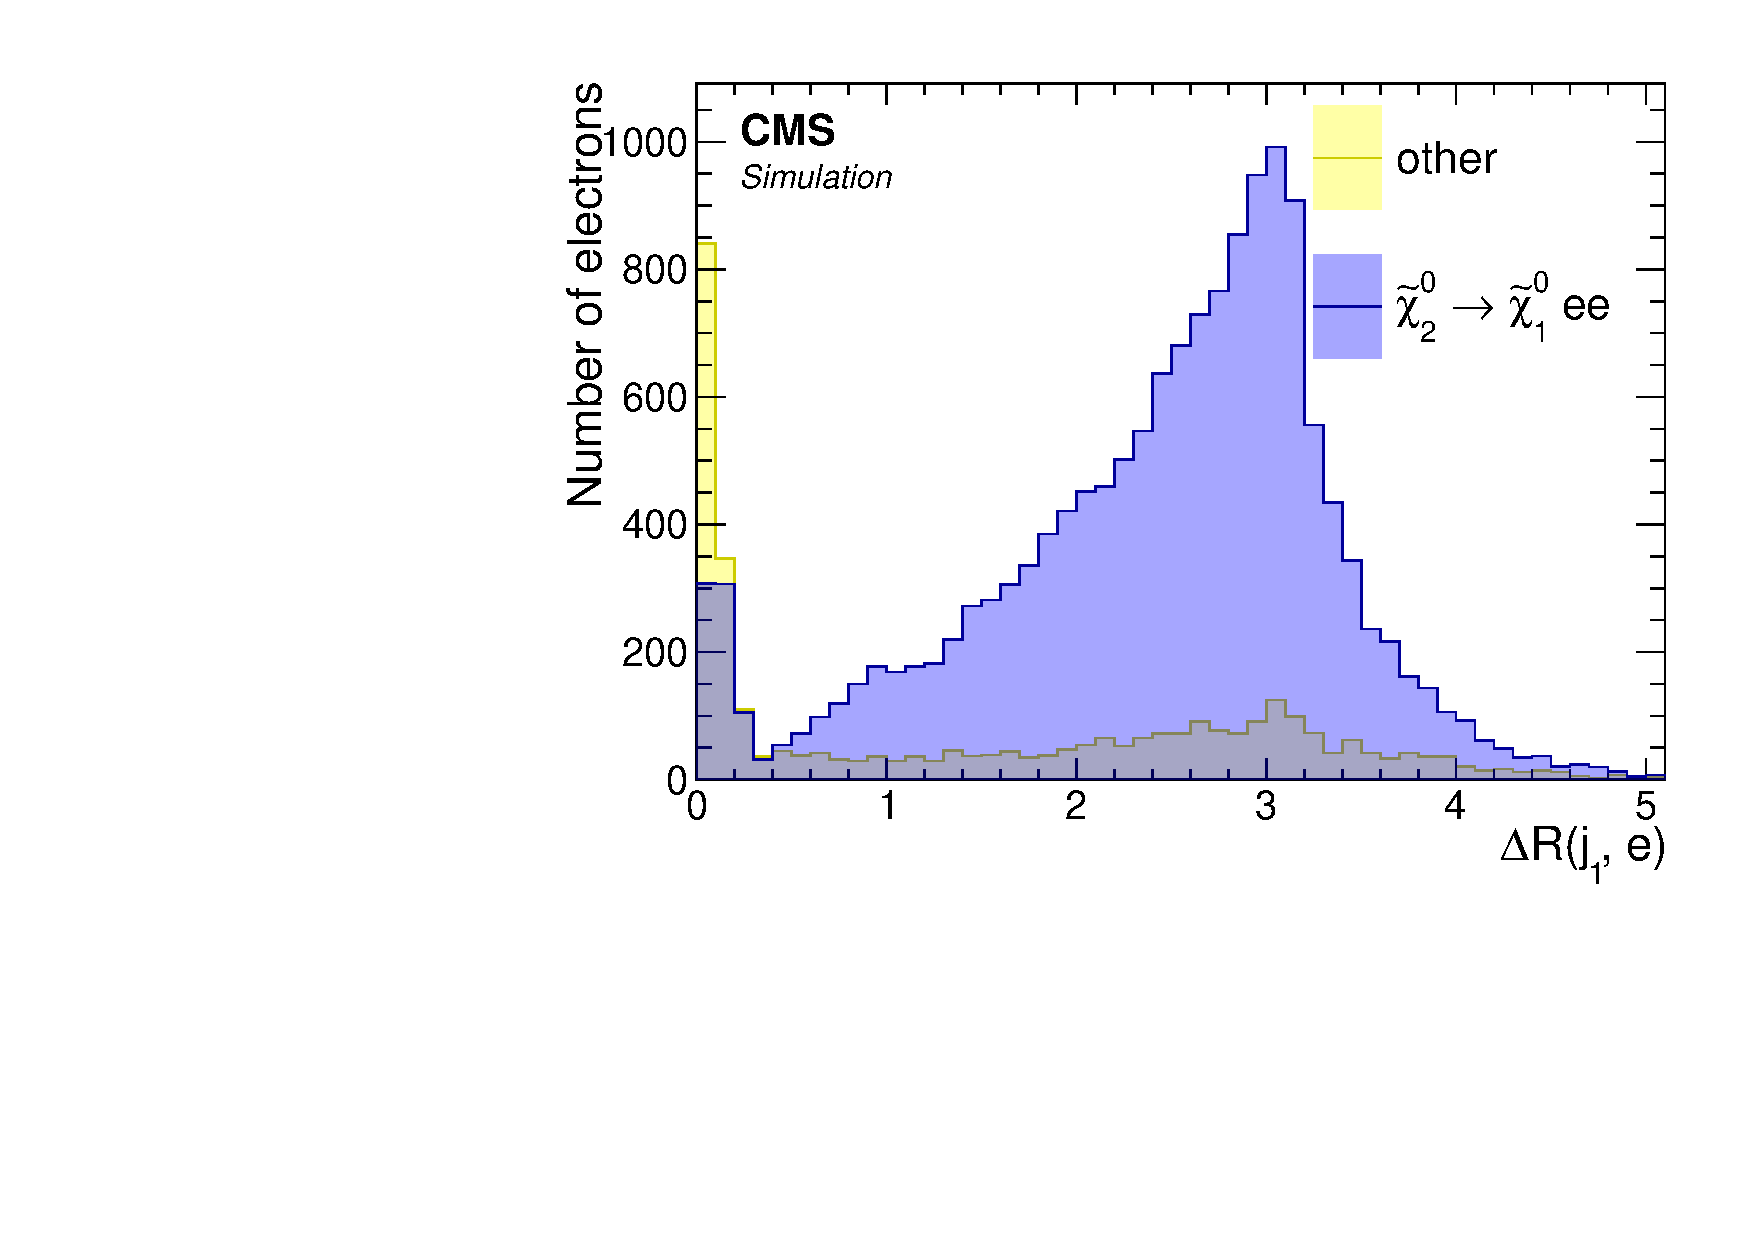
\includegraphics[width=0.48\linewidth]{plots/lepton_selection/lepton_selection_dm5p63/none_Electrons_rlj.pdf} \,
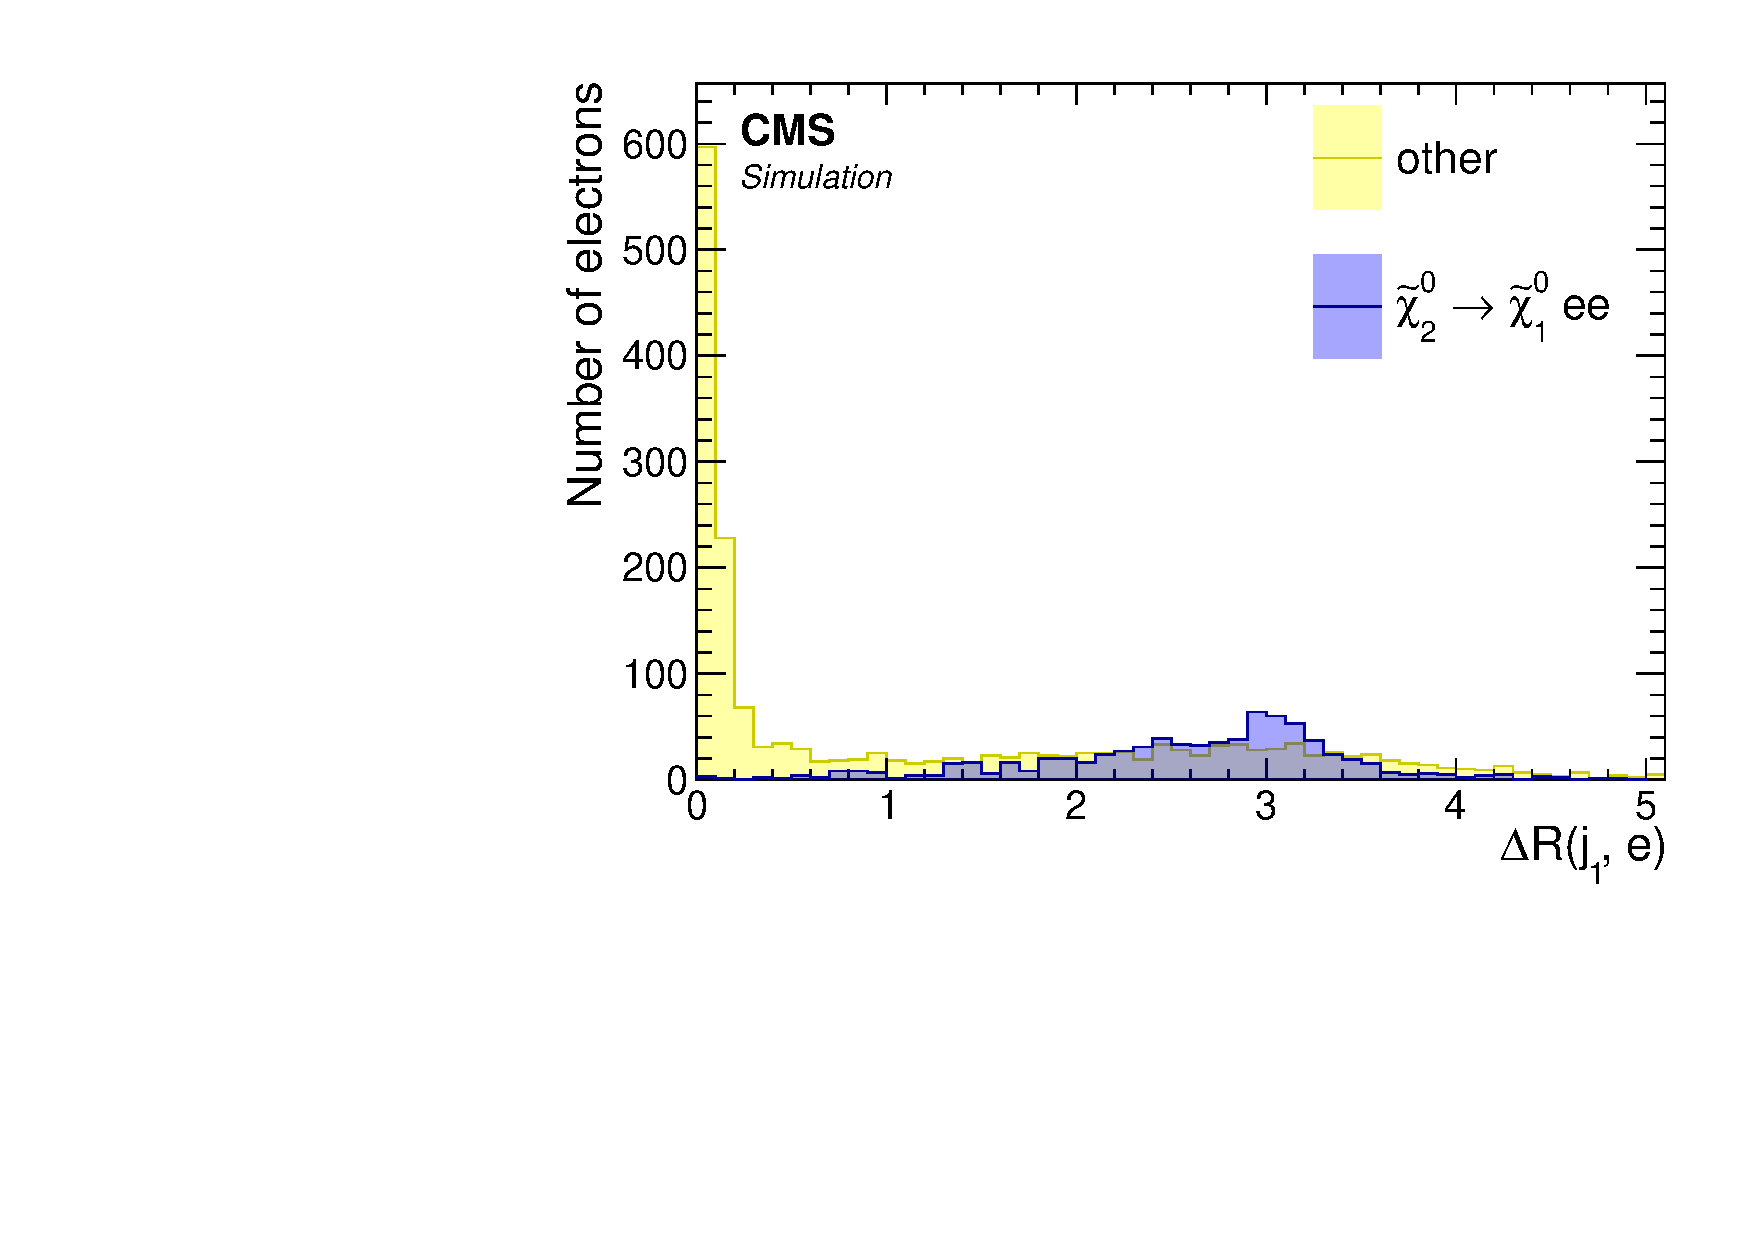
\includegraphics[width=0.48\linewidth]{plots/lepton_selection/lepton_selection_dm1p92/none_Electrons_rlj.pdf}  \\
\caption[Spatial seperation between reconstructed electrons and the leading jet $\DR(\jmath_1,\Pe)$]{Spatial seperation between reconstructed electrons with loose ID and the leading jet $\DR(\jmath_1,\Pe)$ for $\dm=5.63\GeV$ (left) and $\dm=1.92\GeV$ (right).}
\label{fig:electrons-dr-lj}
\end{figure}

There are two obvious features we can take from these plots. The first we have explored already in~\ref{sec:signal-signature}, namely, that probing lower \gls{dm} requires access to low \gls{pt} leptons, and since we are limited by a lower threshold of $\pt\geq 5\GeV$ on the electrons, that results in lower signal acceptance as can be seen by the difference between the high \gls{dm} and the low one. The second interesting feature that we can see, is that our signal electrons are located mainly outside of the leading jet. That is because the leading jet is usually an \gls{isr} jet which boosts the \tchiz system to away from it (back-to-back). We therefore make a cut $\DR(\jmath_1,\Pe)>0.4$.

Next we turn into the \gls{pt} distributions. We apply the previous cut of $\DR(\jmath_1,\Pe)>0.4$. As we've already seen in~\ref{sec:muon-eta-pt}, the \gls{pt} distribution depends strongly on \gls{dm}. Even though the distributions in~\ref{sec:muon-eta-pt} were plotted using generator level muons, the electrons distributions follow the same trend. We therefore need to make a choice about which \gls{dm} to favor, \ie, which \gls{dm} we want to be more sensitive to, and we choose the lower \gls{dm} case. Nonetheless we compare the two choices.

\begin{figure}[!htb]
\centering
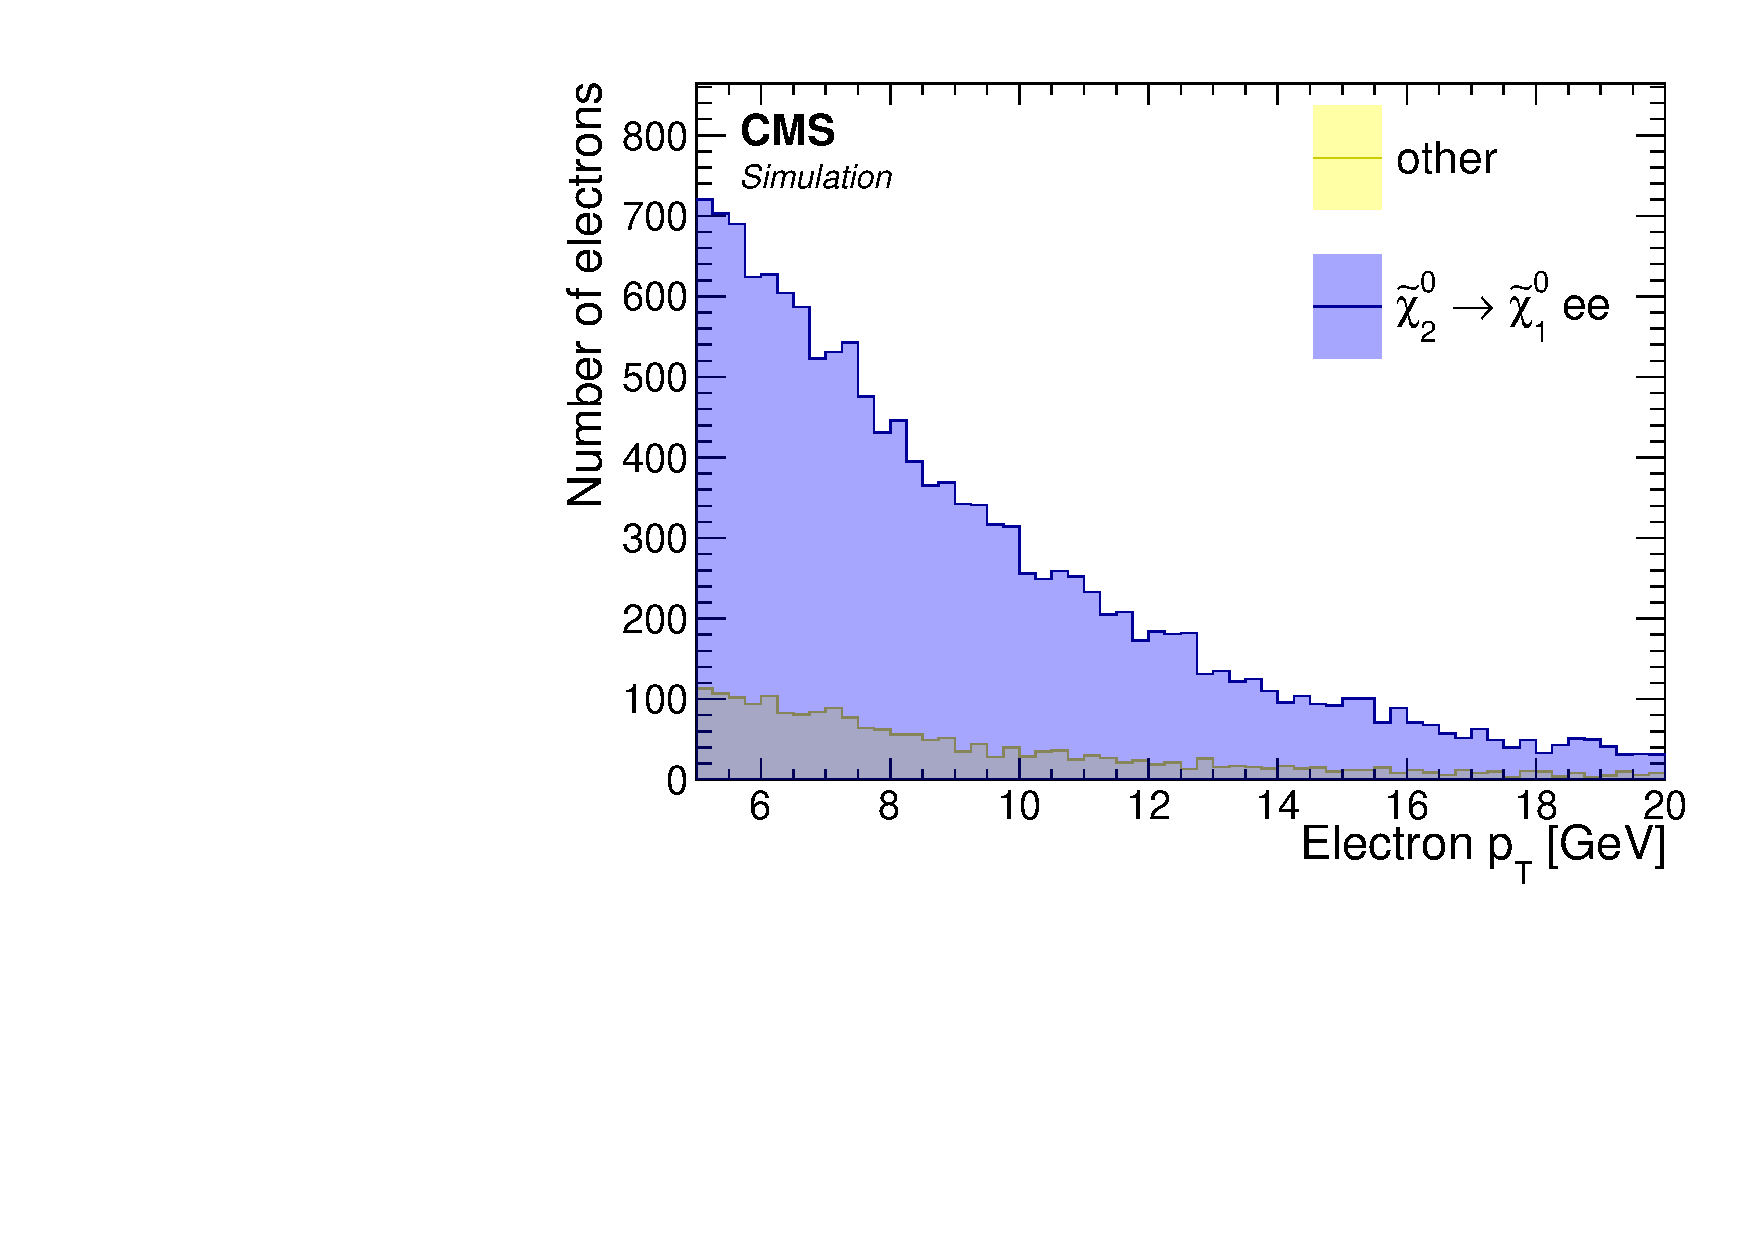
\includegraphics[width=0.48\linewidth]{plots/lepton_selection/lepton_selection_dm5p63/none_Electrons_pt.pdf} \,
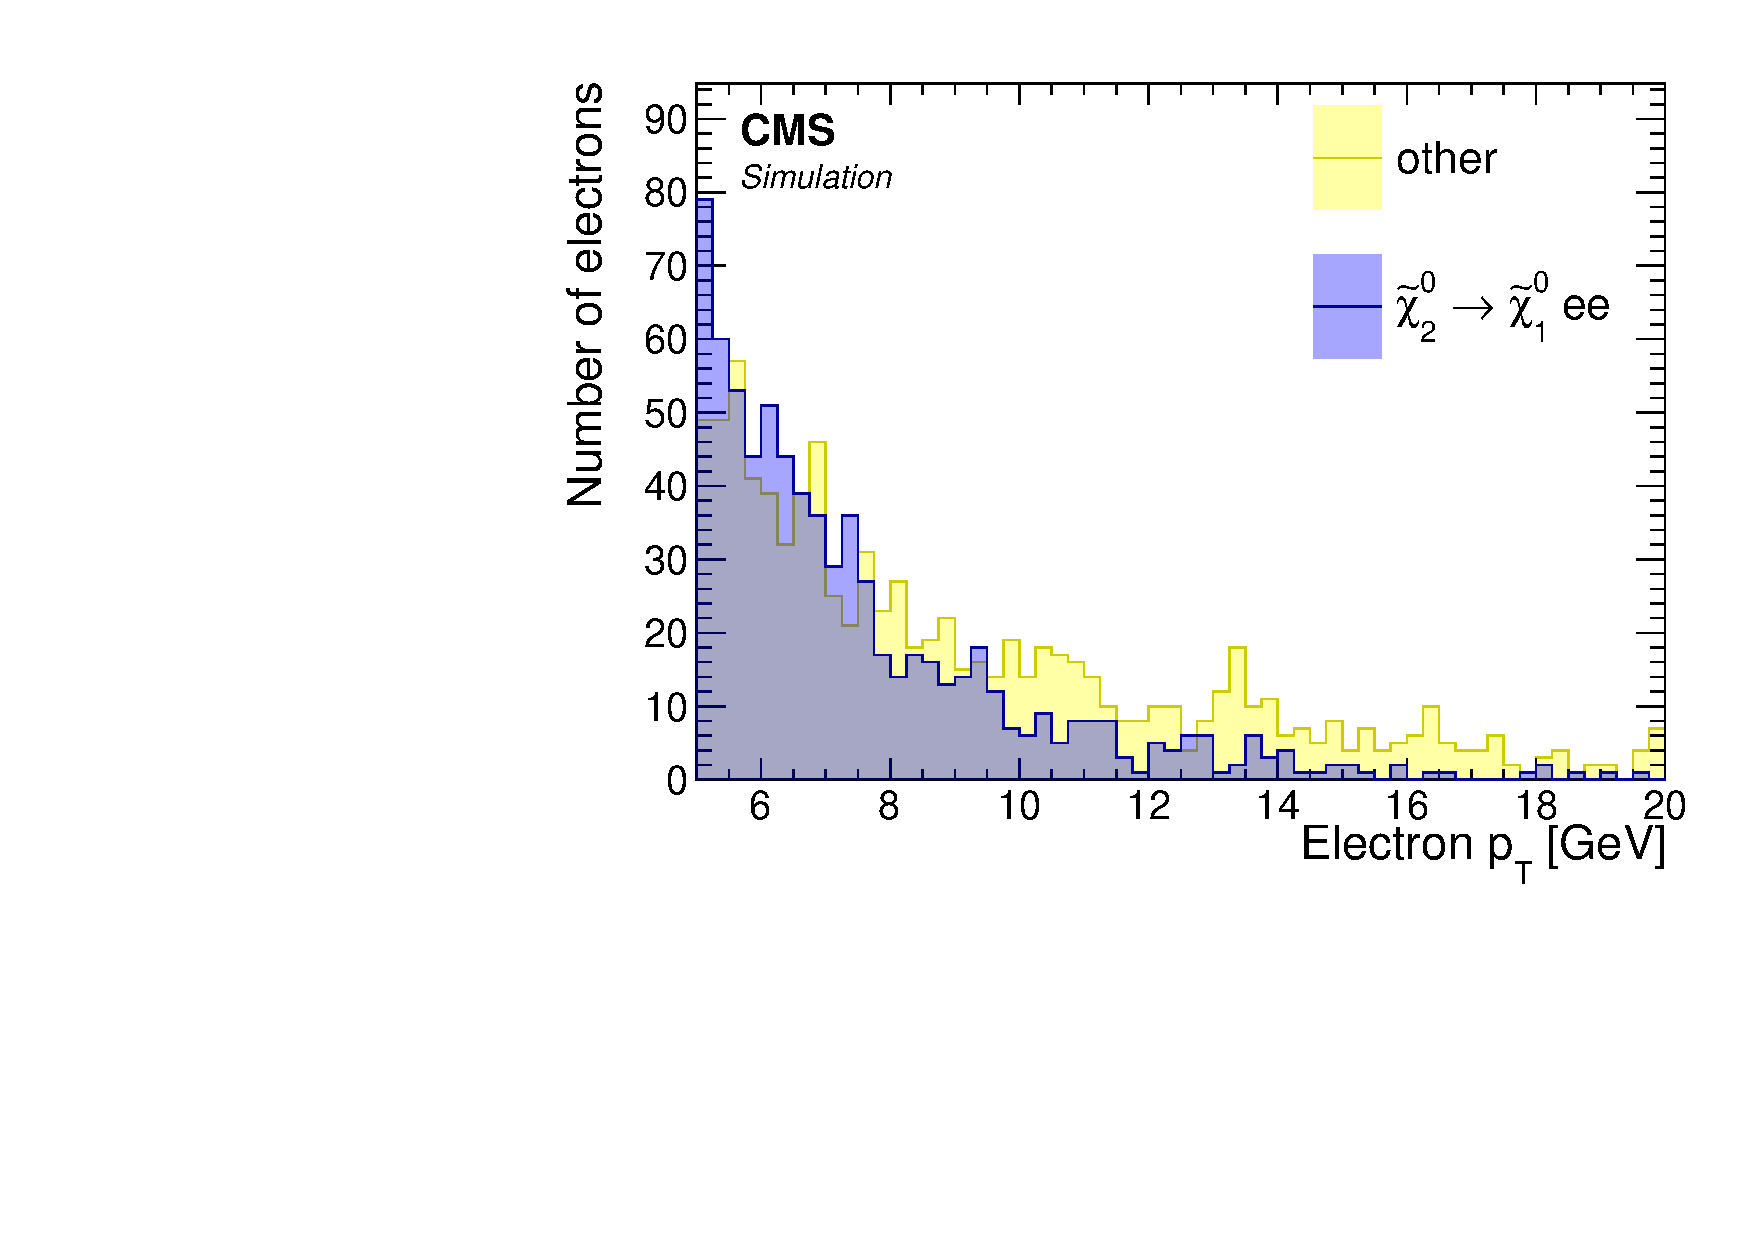
\includegraphics[width=0.48\linewidth]{plots/lepton_selection/lepton_selection_dm1p92/none_Electrons_pt.pdf}  \\
\caption[\pt distribution of reconstructed electrons with loose ID]{ \pt distribution of reconstructed electrons with loose ID for $\dm=5.63\GeV$ (left) and $\dm=1.92\GeV$ (right). Cut of $\DR(\jmath_1,\Pe)>0.4$ applied.}
\label{fig:electrons-selection-pt}
\end{figure}

We can see, as expected, that the \pt distribution  of the electrons fall more rapidly for the low \dm case. We observe that there are hardly any electrons surviving above $15\GeV$, and therefore we choose to make a cut of $\pt<15\GeV$.

It interesting to look at the $\eta$ distribution after the previous cuts to get a better sense of where most of the non-signal electrons are stil coming from.

\begin{figure}[!htb]
\centering
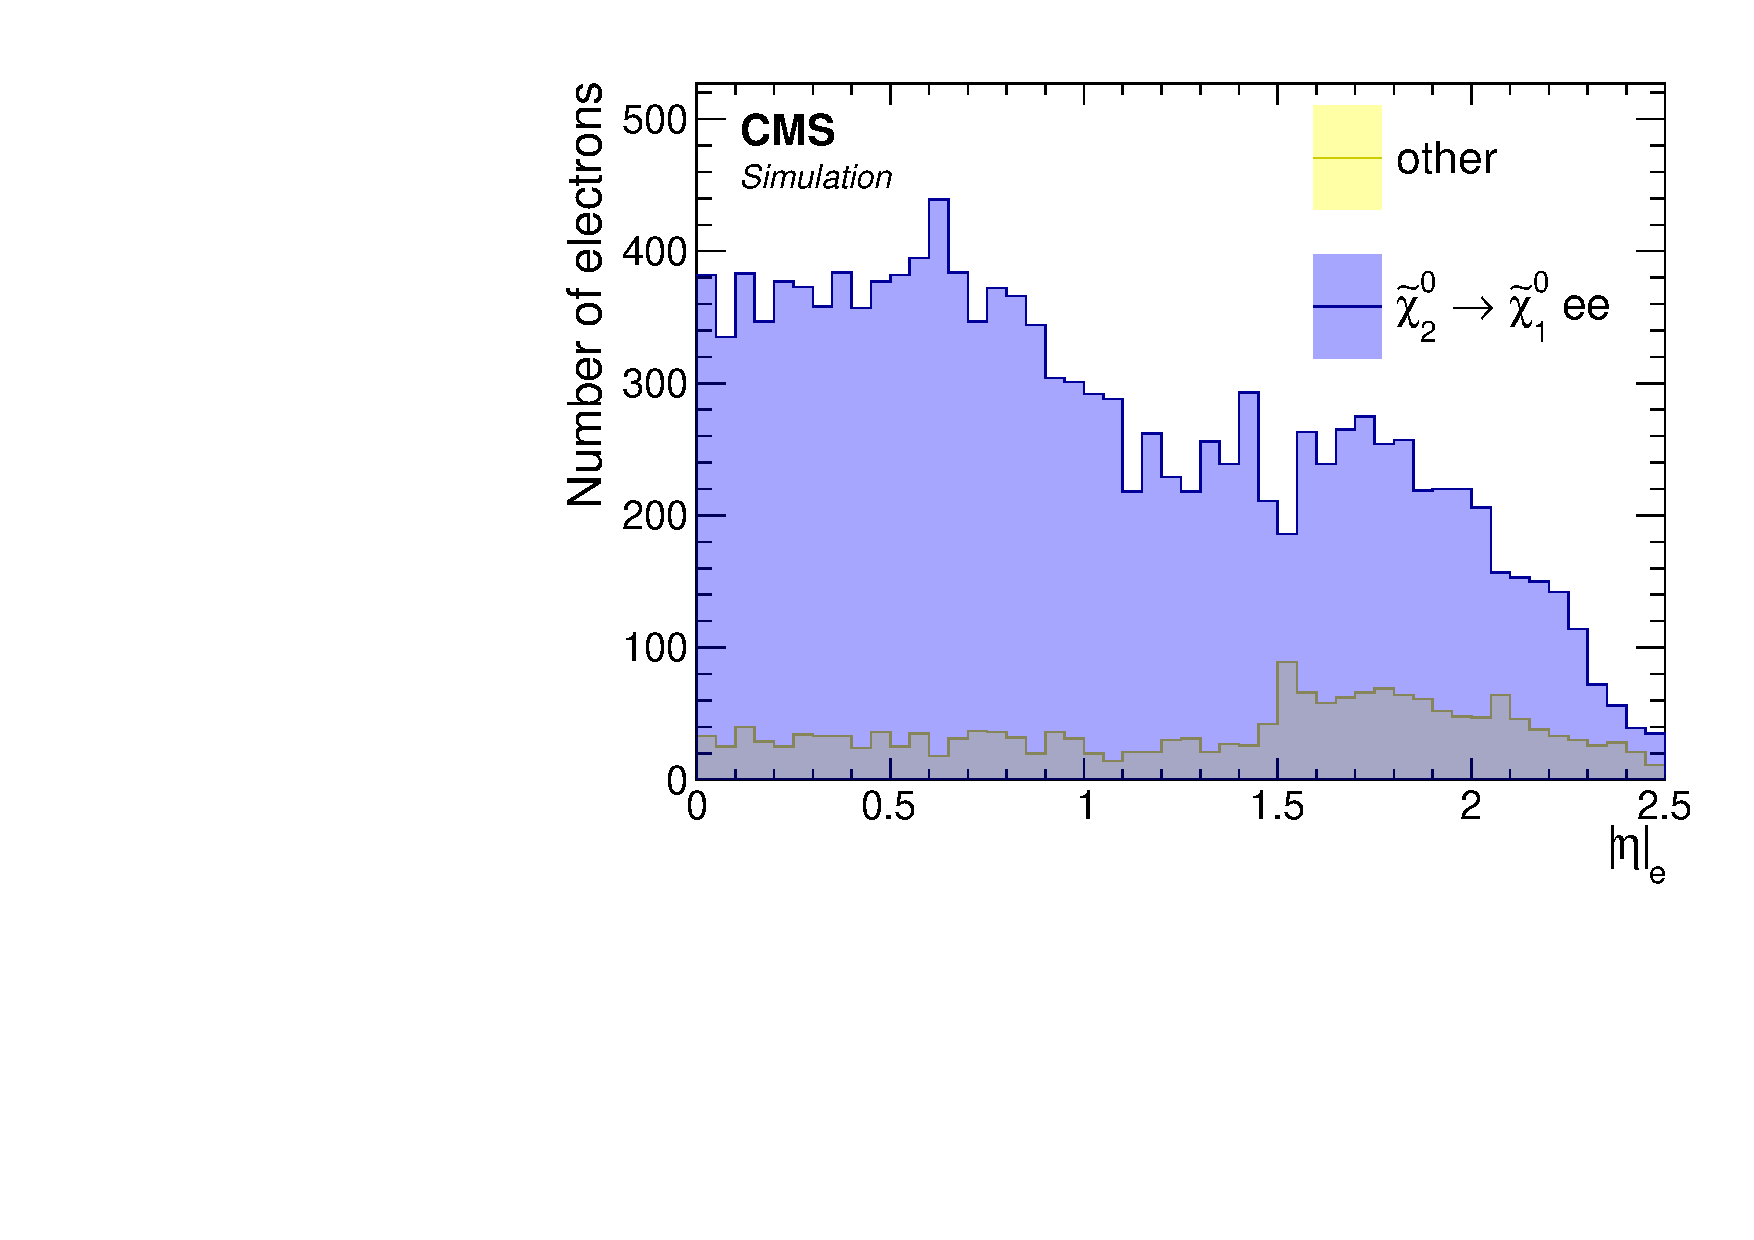
\includegraphics[width=0.48\linewidth]{plots/lepton_selection/lepton_selection_dm5p63/none_Electrons_eta.pdf} \,
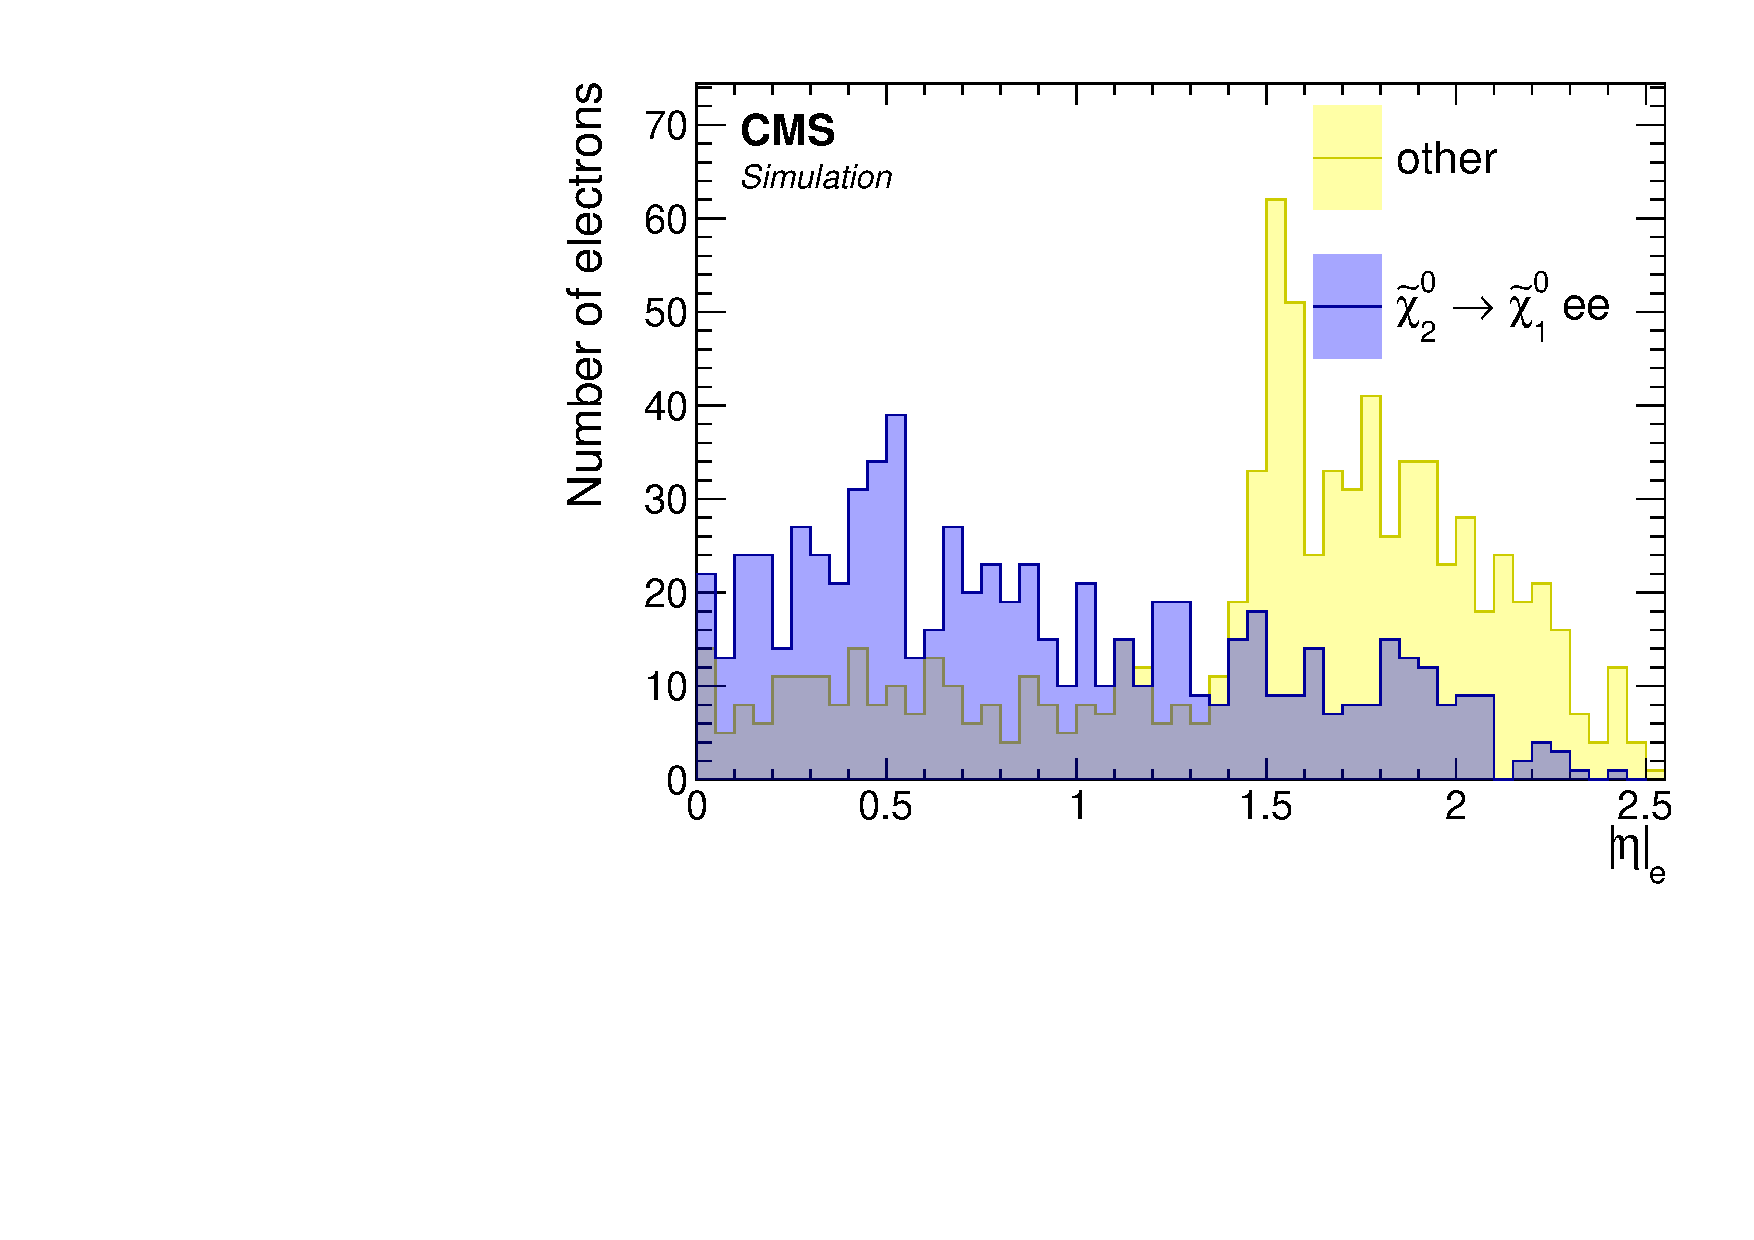
\includegraphics[width=0.48\linewidth]{plots/lepton_selection/lepton_selection_dm1p92/none_Electrons_eta.pdf}  \\
\caption[\abs{\eta} distribution of reconstructed electrons with loose ID]{ \abs{\eta} distribution of reconstructed electrons with loose ID for $\dm=5.63\GeV$ (left) and $\dm=1.92\GeV$ (right). Cuts of $\DR(\jmath_1,\Pe)>0.4$ and $\pt<15\GeV$ are applied.}
\label{fig:electrons-selection-eta}
\end{figure}

In the case of $\dm=1.92\GeV$,  we can clearly see how worse the endcaps of the \gls{ecal} are performing in comparison with the barrel ($\abs{\eta}<1.48$). The transition is clearly visible through a sharp drop in purity at the transition. It is worse for low-\pt electrons than higher-\pt ones.

We would like to see if requiring a tighter working point for the electron-identification is beneficial. The working point used in the previous distributions is loose. We look turn now to check the effects of requiring either a medium working point, or a tight one. We plot two bins labeled \emph{fail} and \emph{pass}, which correspond to whether the electron passes or failed the identification criteria of a medium or tight working points.

\begin{figure}[!htb]
\centering
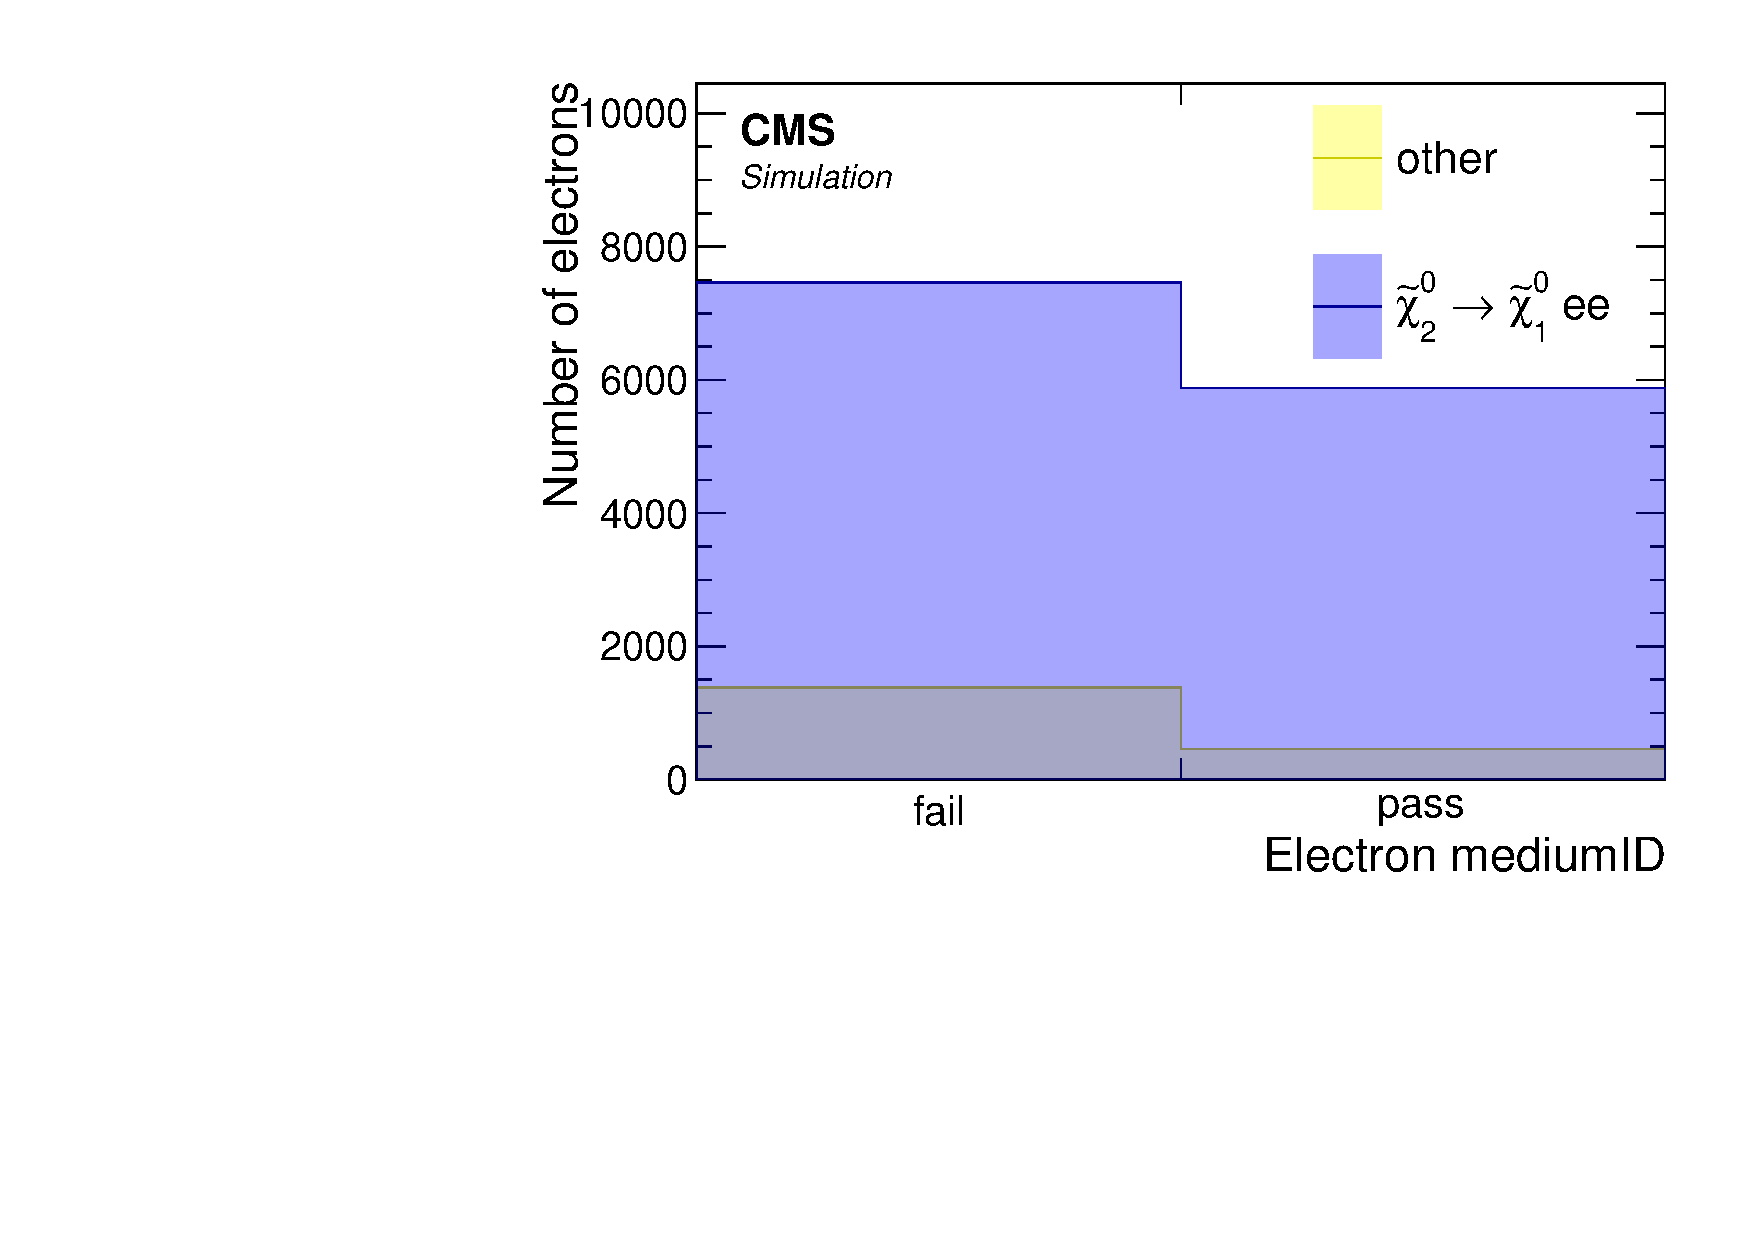
\includegraphics[width=0.48\linewidth]{plots/lepton_selection/lepton_selection_dm5p63/none_Electrons_medium.pdf} \,
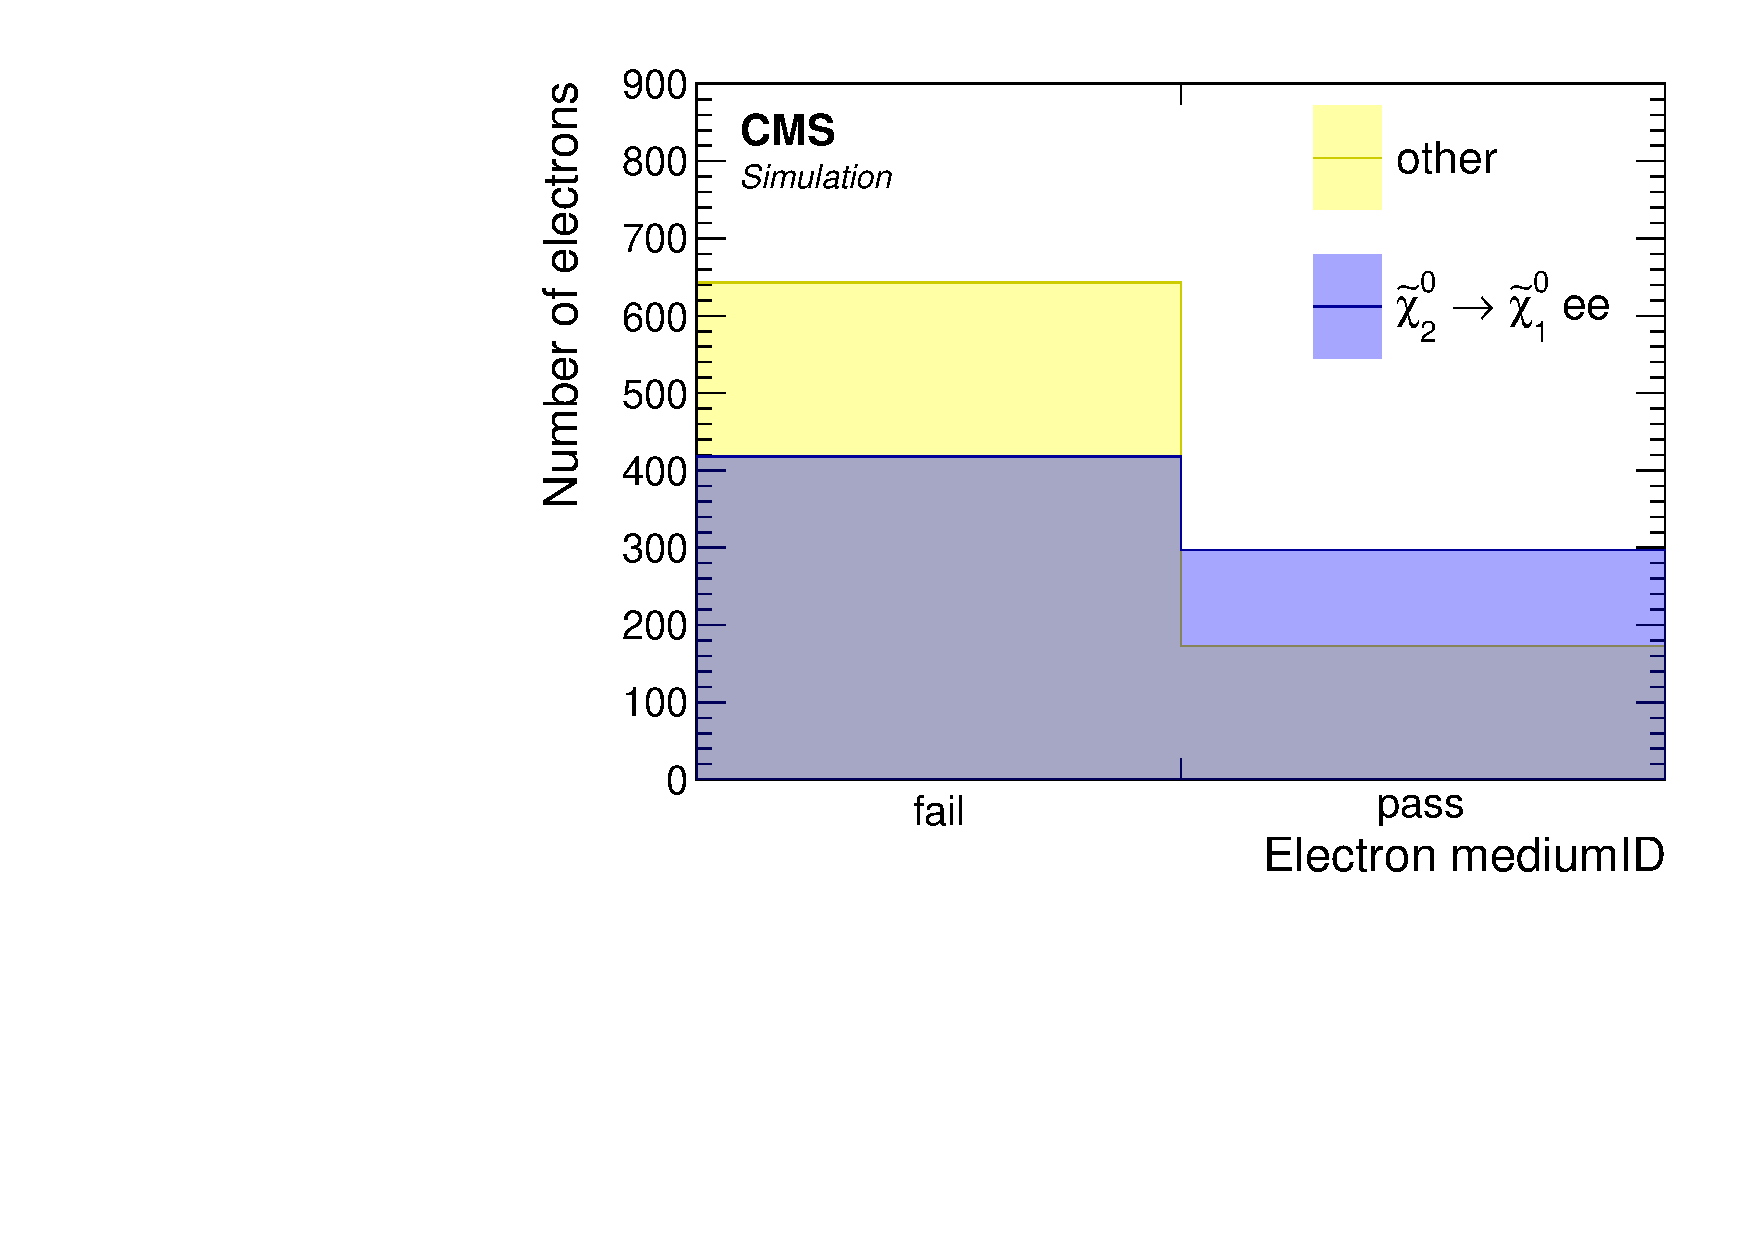
\includegraphics[width=0.48\linewidth]{plots/lepton_selection/lepton_selection_dm1p92/none_Electrons_medium.pdf}  \\
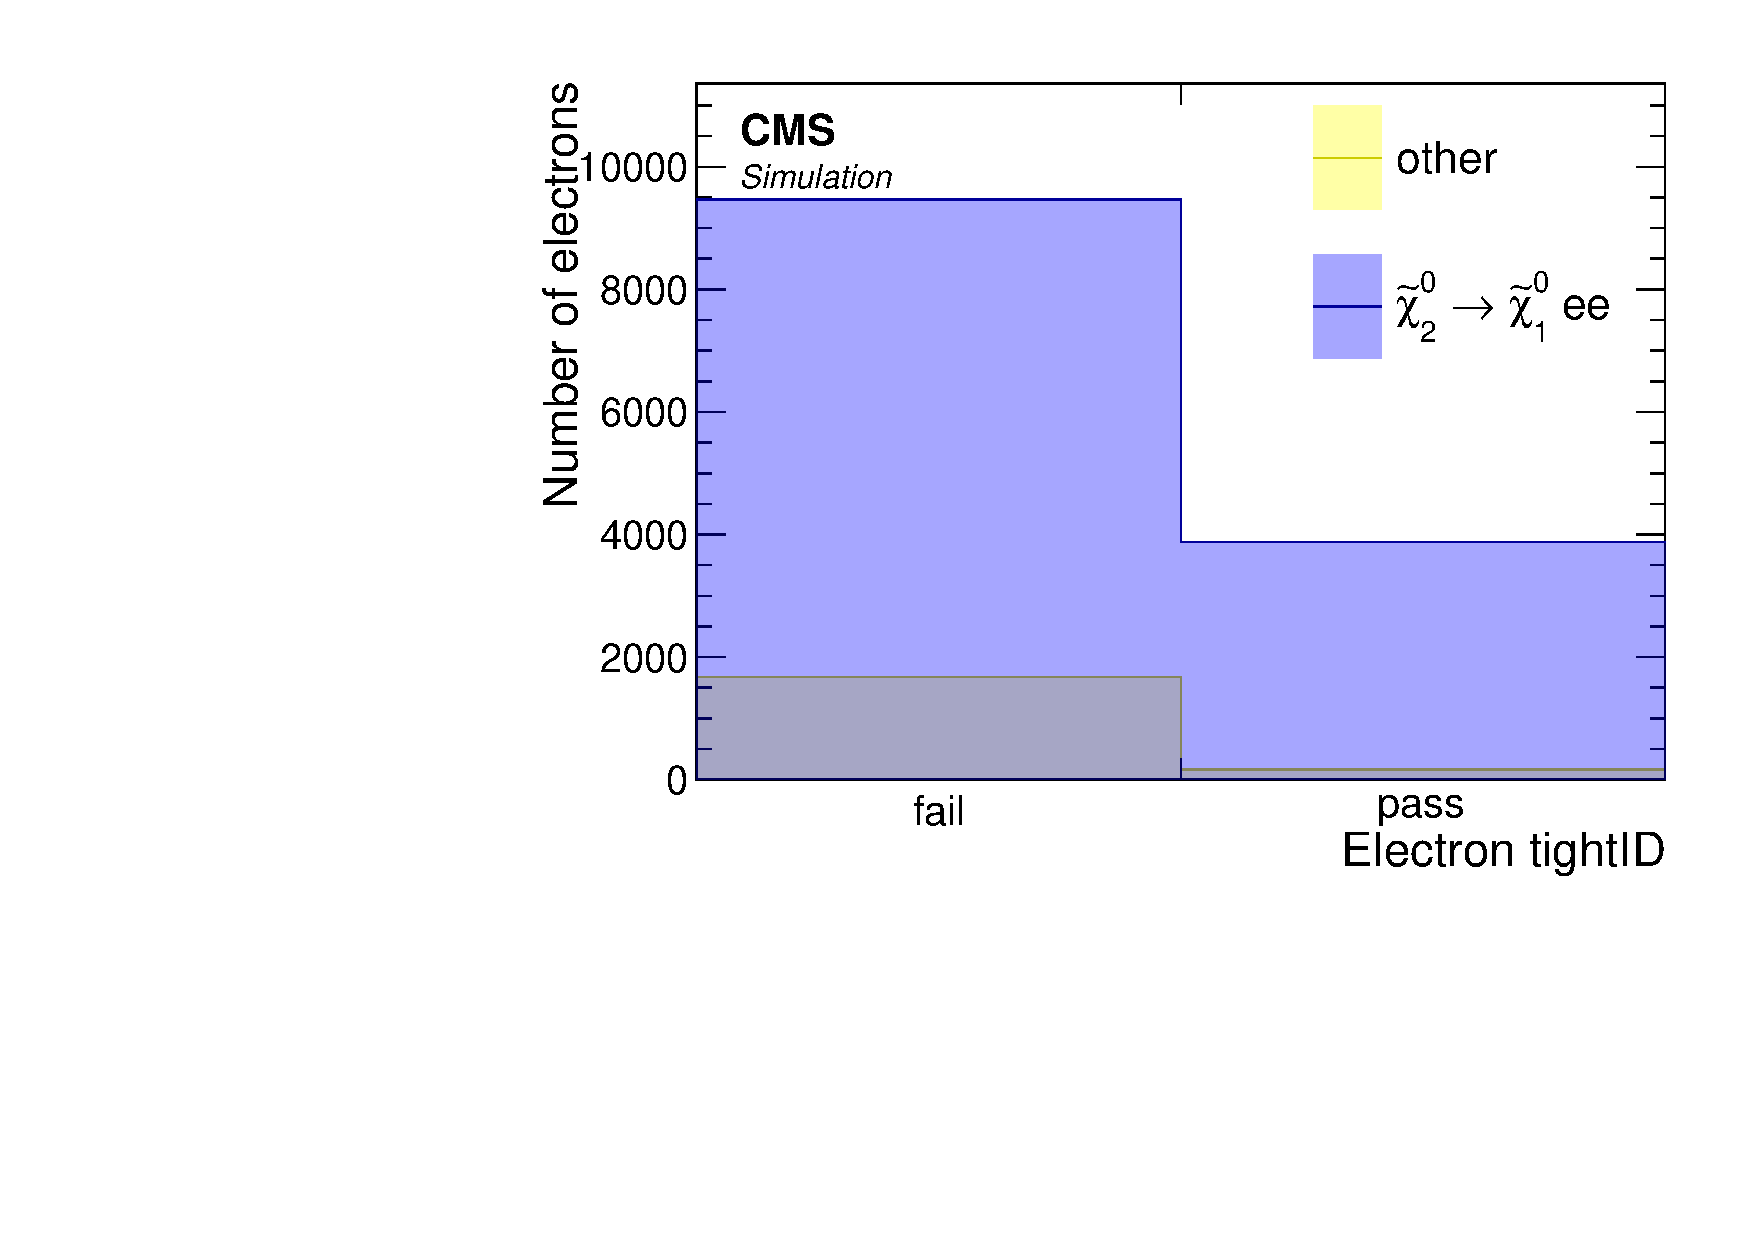
\includegraphics[width=0.48\linewidth]{plots/lepton_selection/lepton_selection_dm5p63/none_Electrons_tight.pdf} \,
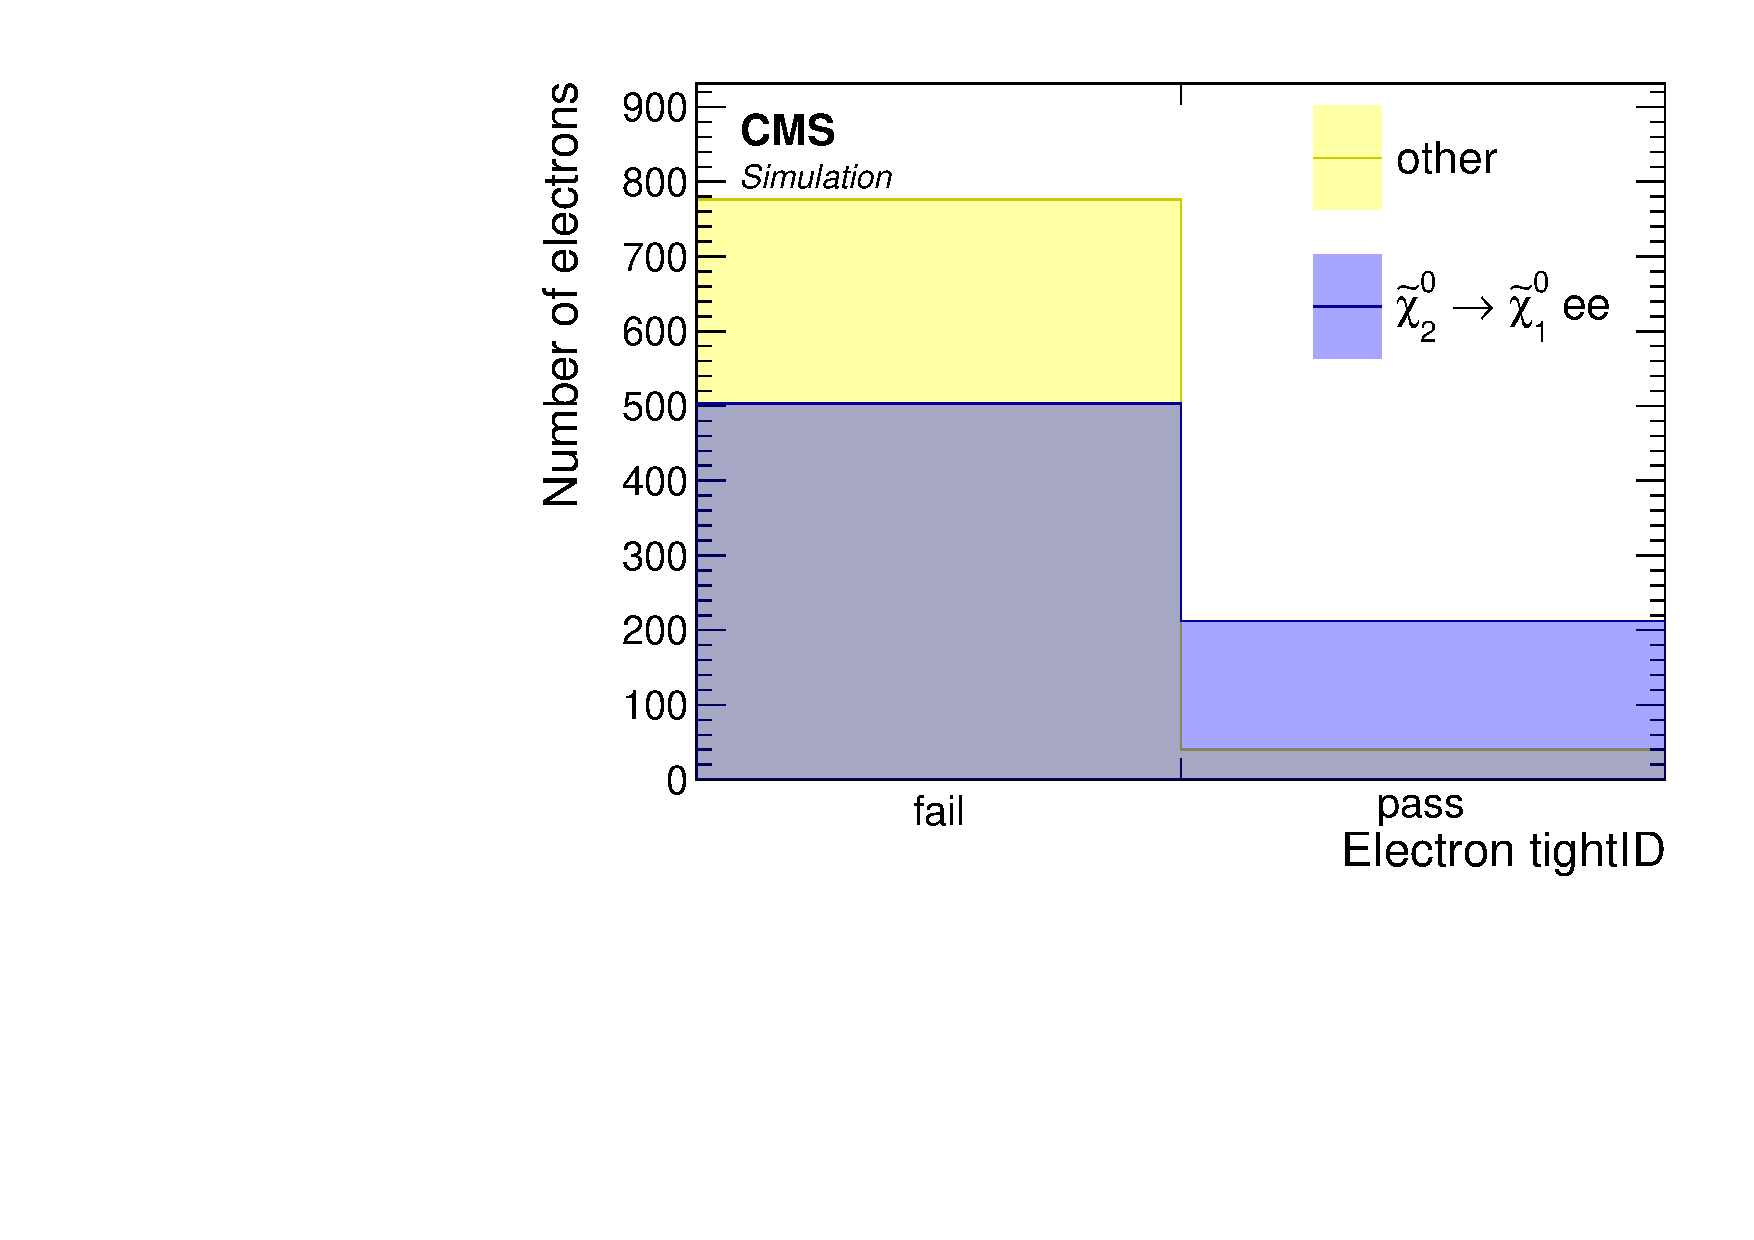
\includegraphics[width=0.48\linewidth]{plots/lepton_selection/lepton_selection_dm1p92/none_Electrons_tight.pdf}  \\
\caption[medium and tight ID working points distribution of reconstructed electrons]{Medium (top) and tight (bottom) ID working points distributions of reconstructed electrons for $\dm=5.63\GeV$ (left) and $\dm=1.92\GeV$ (right). Cuts of $\DR(\jmath_1,\Pe)>0.4$ and $\pt<15\GeV$ are applied.}
\label{fig:electrons-selection-id}
\end{figure}

Selecting a medium or a tight working point is equivalent to choosing the relevant right \emph{pass} bin (top for medium, bottom for tight), and rejecting the electrons on the left \emph{fail} bin. We see that although we reject considerable amount of non-signal electrons in the low \dm case by picking either a medium or tight working points, we also loose quite a lot of signal electrons as well. In other words, these selections are very not efficient and will result in low signal acceptance. We therefore decide to use a loose working point for the electrons. We will see that we can still purify the electron selection by relying on isolation instead. We fully discuss and describe our jet-isolation in~\ref{sec:isolation}, but here for the sake of completeness we look at its effect on the purity of the electrons. We compare our custom jet-isolation to the standard definition of lepton isolation, which does not take into account the possibility that two electrons can be produced close to each other (small \DR), as is the case in our signal.

\begin{figure}[!htb]
\centering
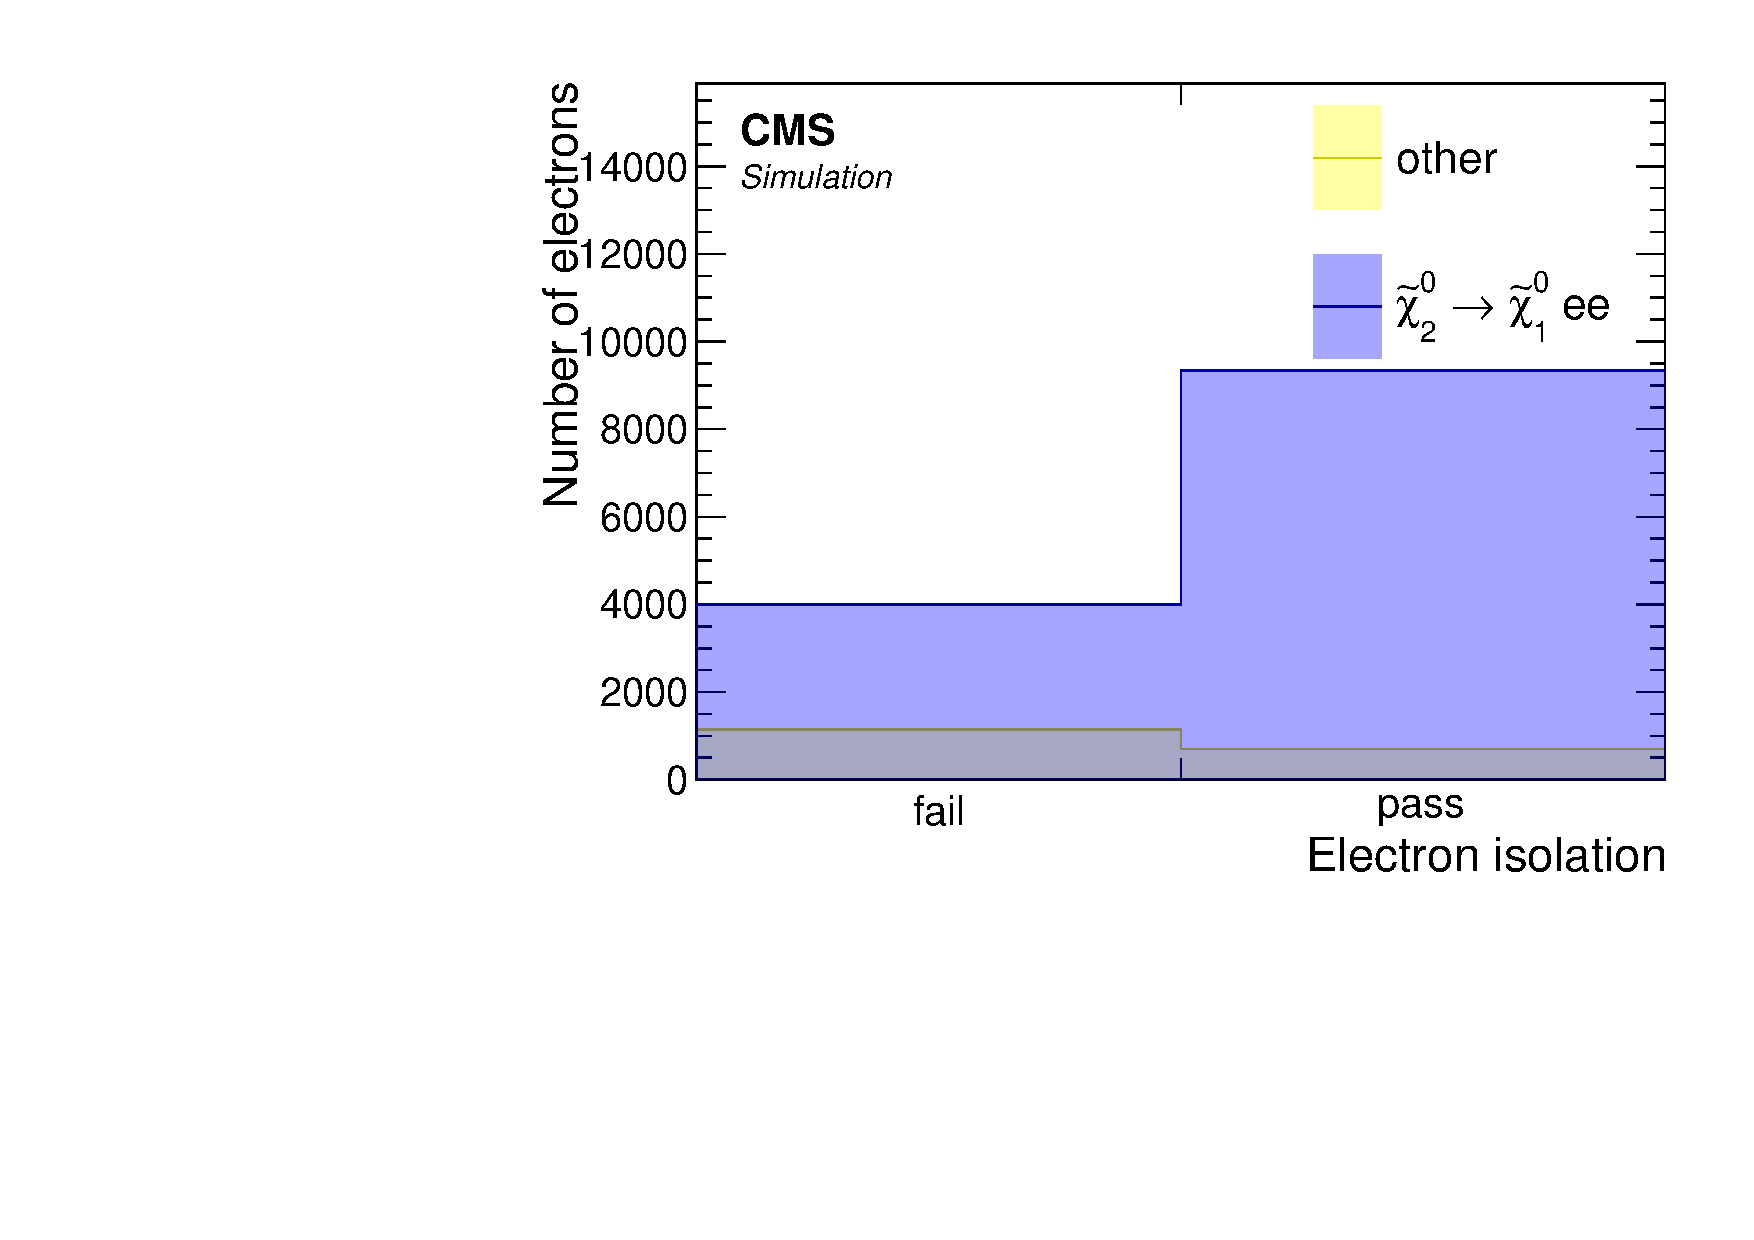
\includegraphics[width=0.48\linewidth]{plots/lepton_selection/lepton_selection_dm5p63/none_Electrons_iso.pdf} \,
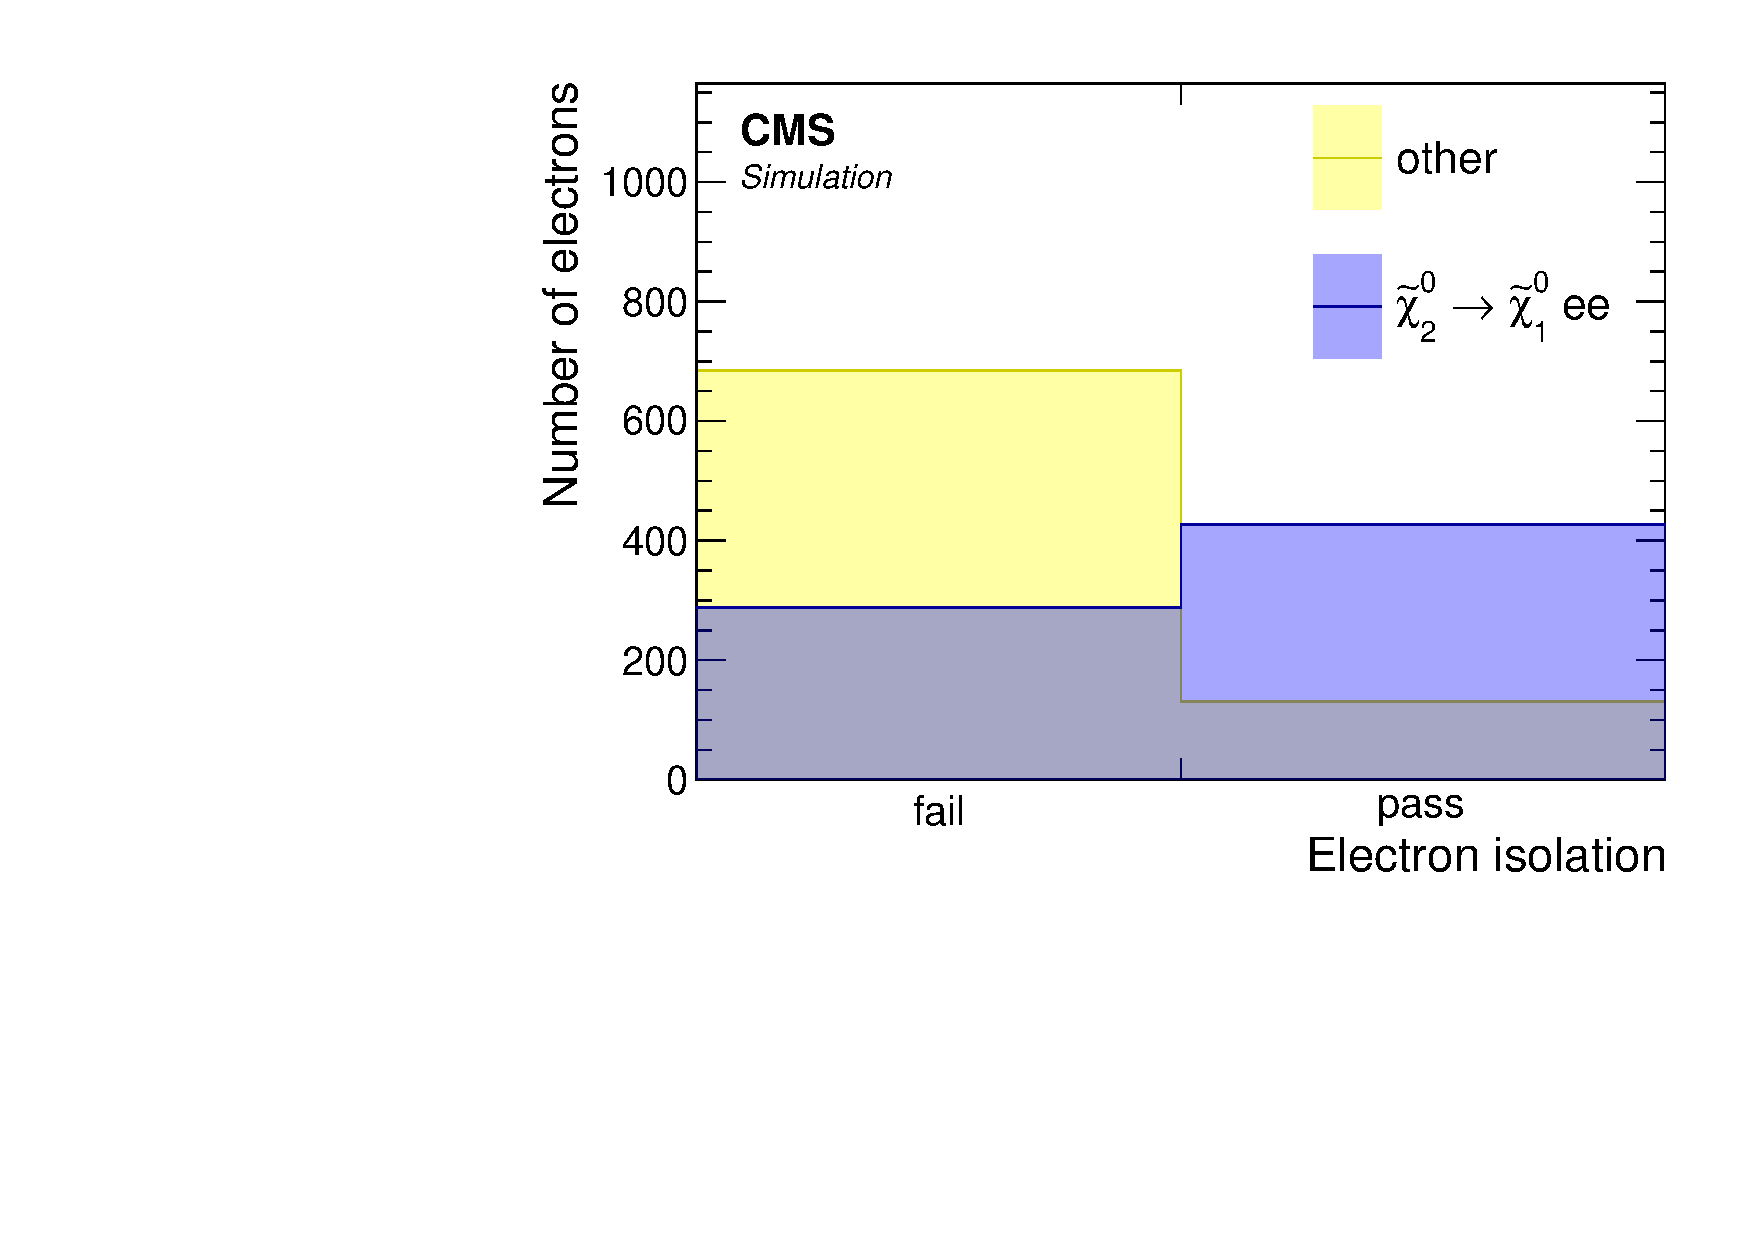
\includegraphics[width=0.48\linewidth]{plots/lepton_selection/lepton_selection_dm1p92/none_Electrons_iso.pdf}  \\
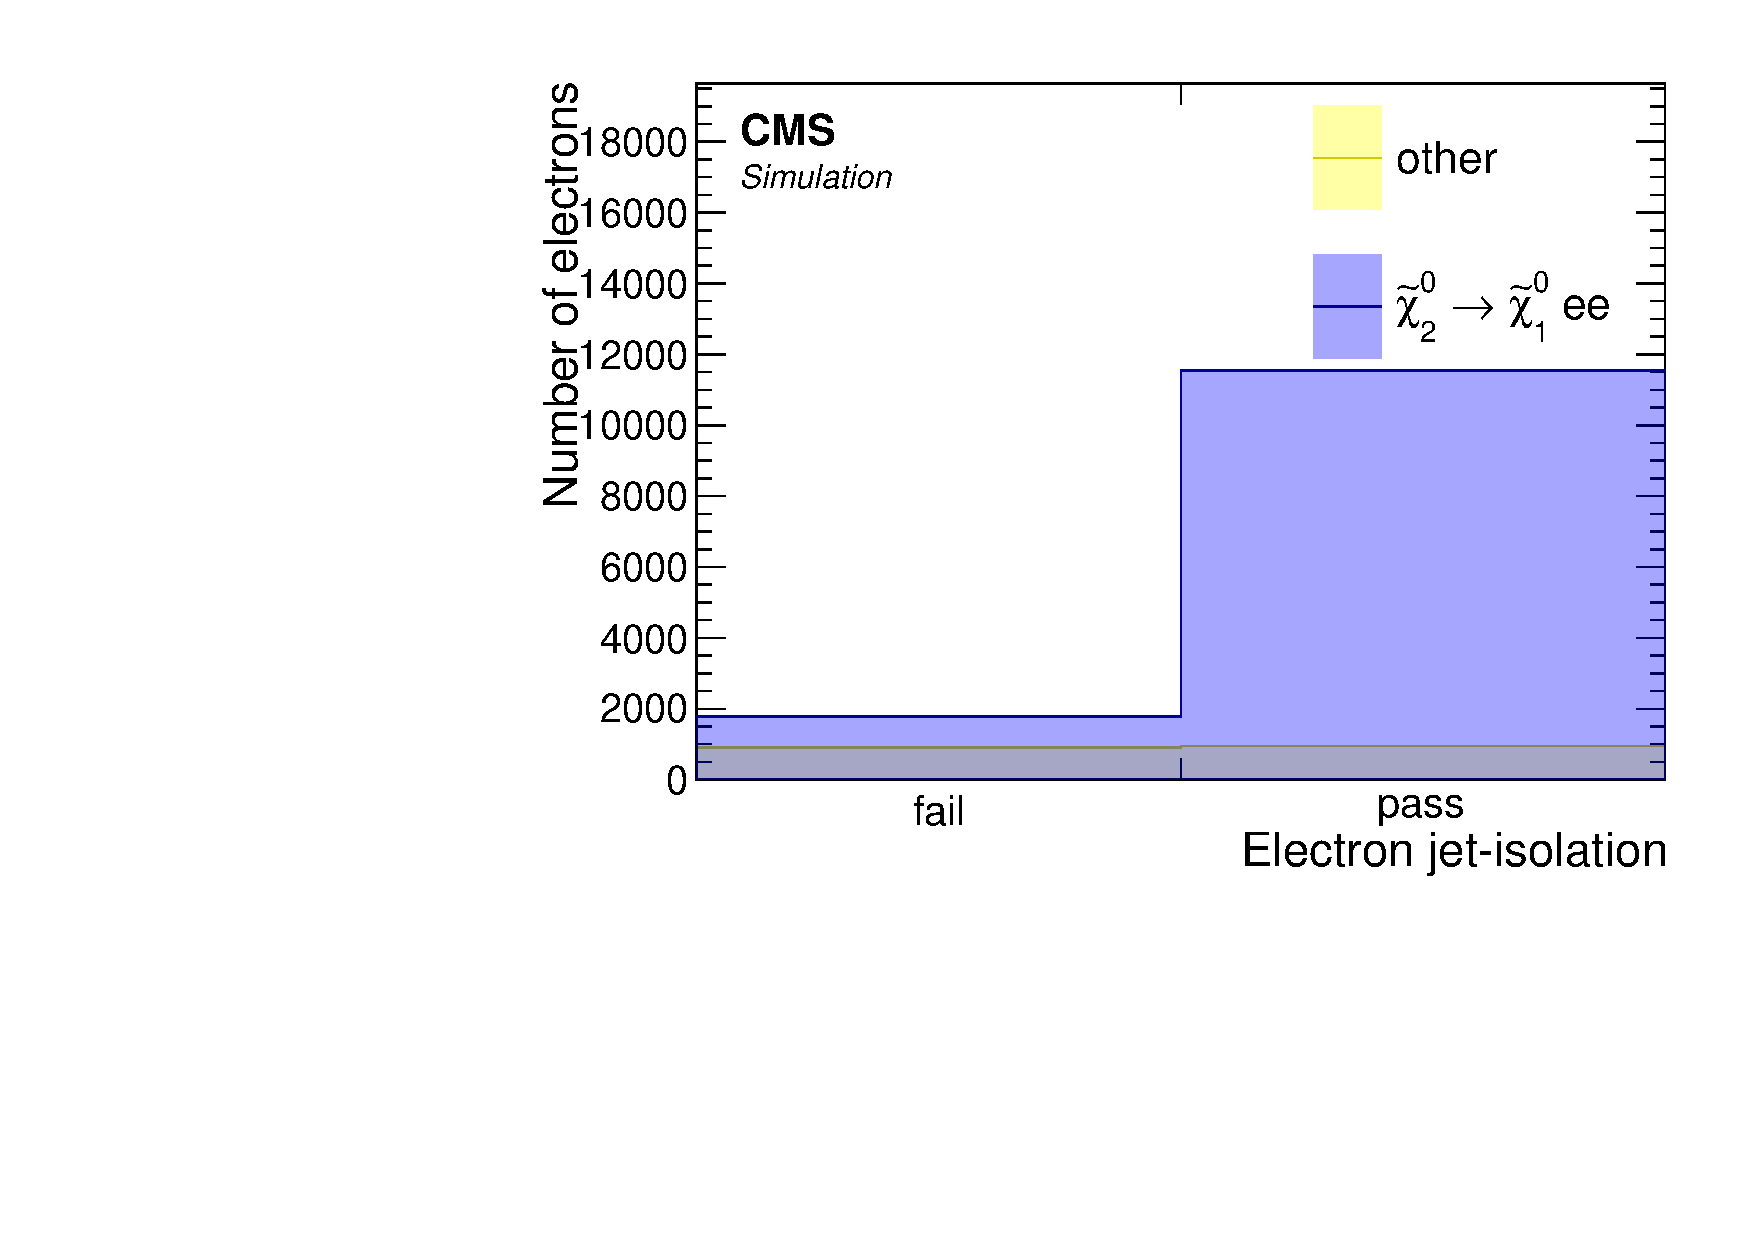
\includegraphics[width=0.48\linewidth]{plots/lepton_selection/lepton_selection_dm5p63/none_Electrons_CorrJetNoMultIso11Dr0.5.pdf} \,
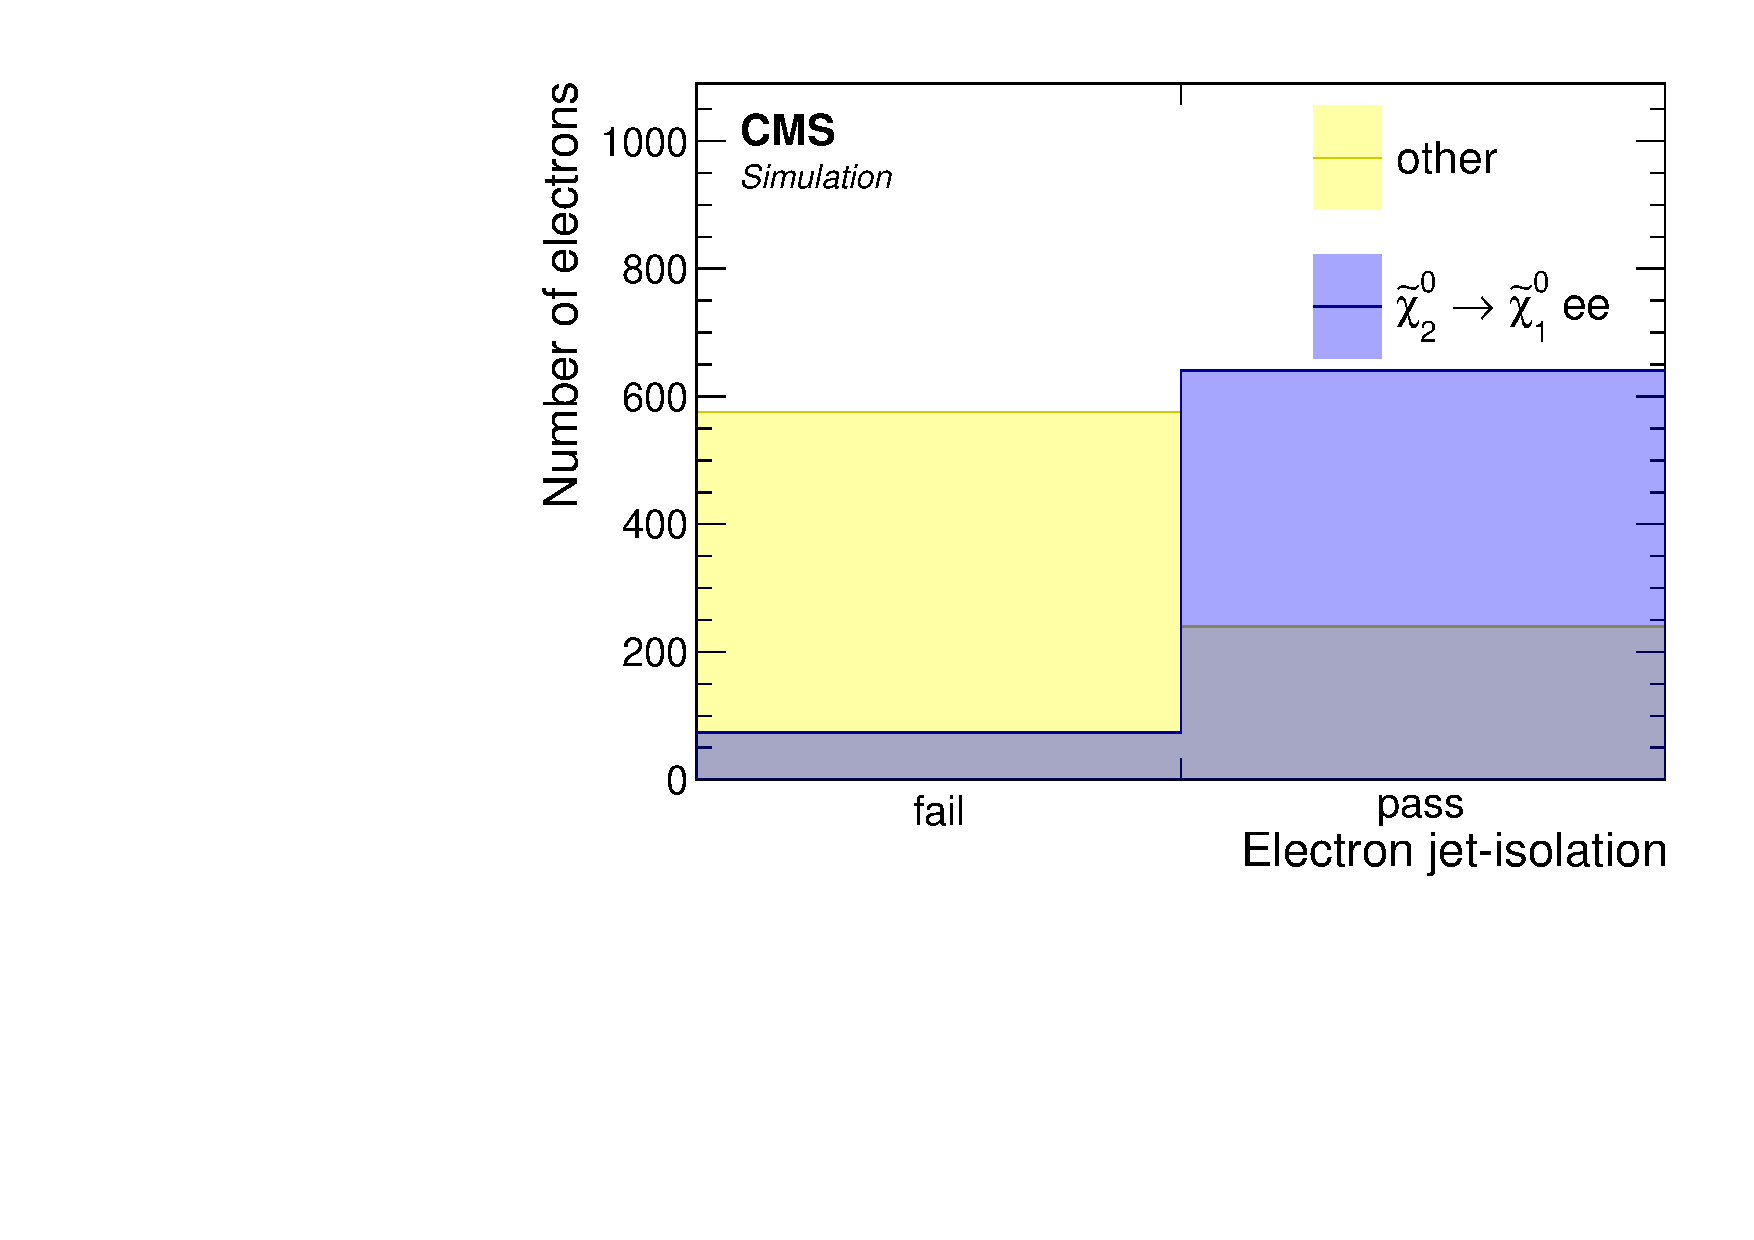
\includegraphics[width=0.48\linewidth]{plots/lepton_selection/lepton_selection_dm1p92/none_Electrons_CorrJetNoMultIso11Dr0.5.pdf}  \\
\caption[standard isolation and jet-isolation distribution of reconstructed electrons]{Standard isolation (top) and custom jet-isolation (bottom) distributions of reconstructed electrons with loose ID for $\dm=5.63\GeV$ (left) and $\dm=1.92\GeV$ (right). Cuts of $\DR(\jmath_1,\Pe)>0.4$ and $\pt<15\GeV$ are applied.}
\label{fig:electrons-selection-isolation}
\end{figure}

We observe that the standard lepton isolation does not perform well in terms of efficiency for both \dm cases. In contrast, the custom jet-isolation is performing very well in terms of signal electron efficiency while successfully rejecting considerable amount of non-signal electrons, resulting in a purer sample of electrons. We therefore conclude that the choice of the custom jet-isolation is favorable. We can look at how the $\eta$ distribution is affected by this choice and that will conclude our selection of the electrons.

\begin{figure}[!htb]
\centering
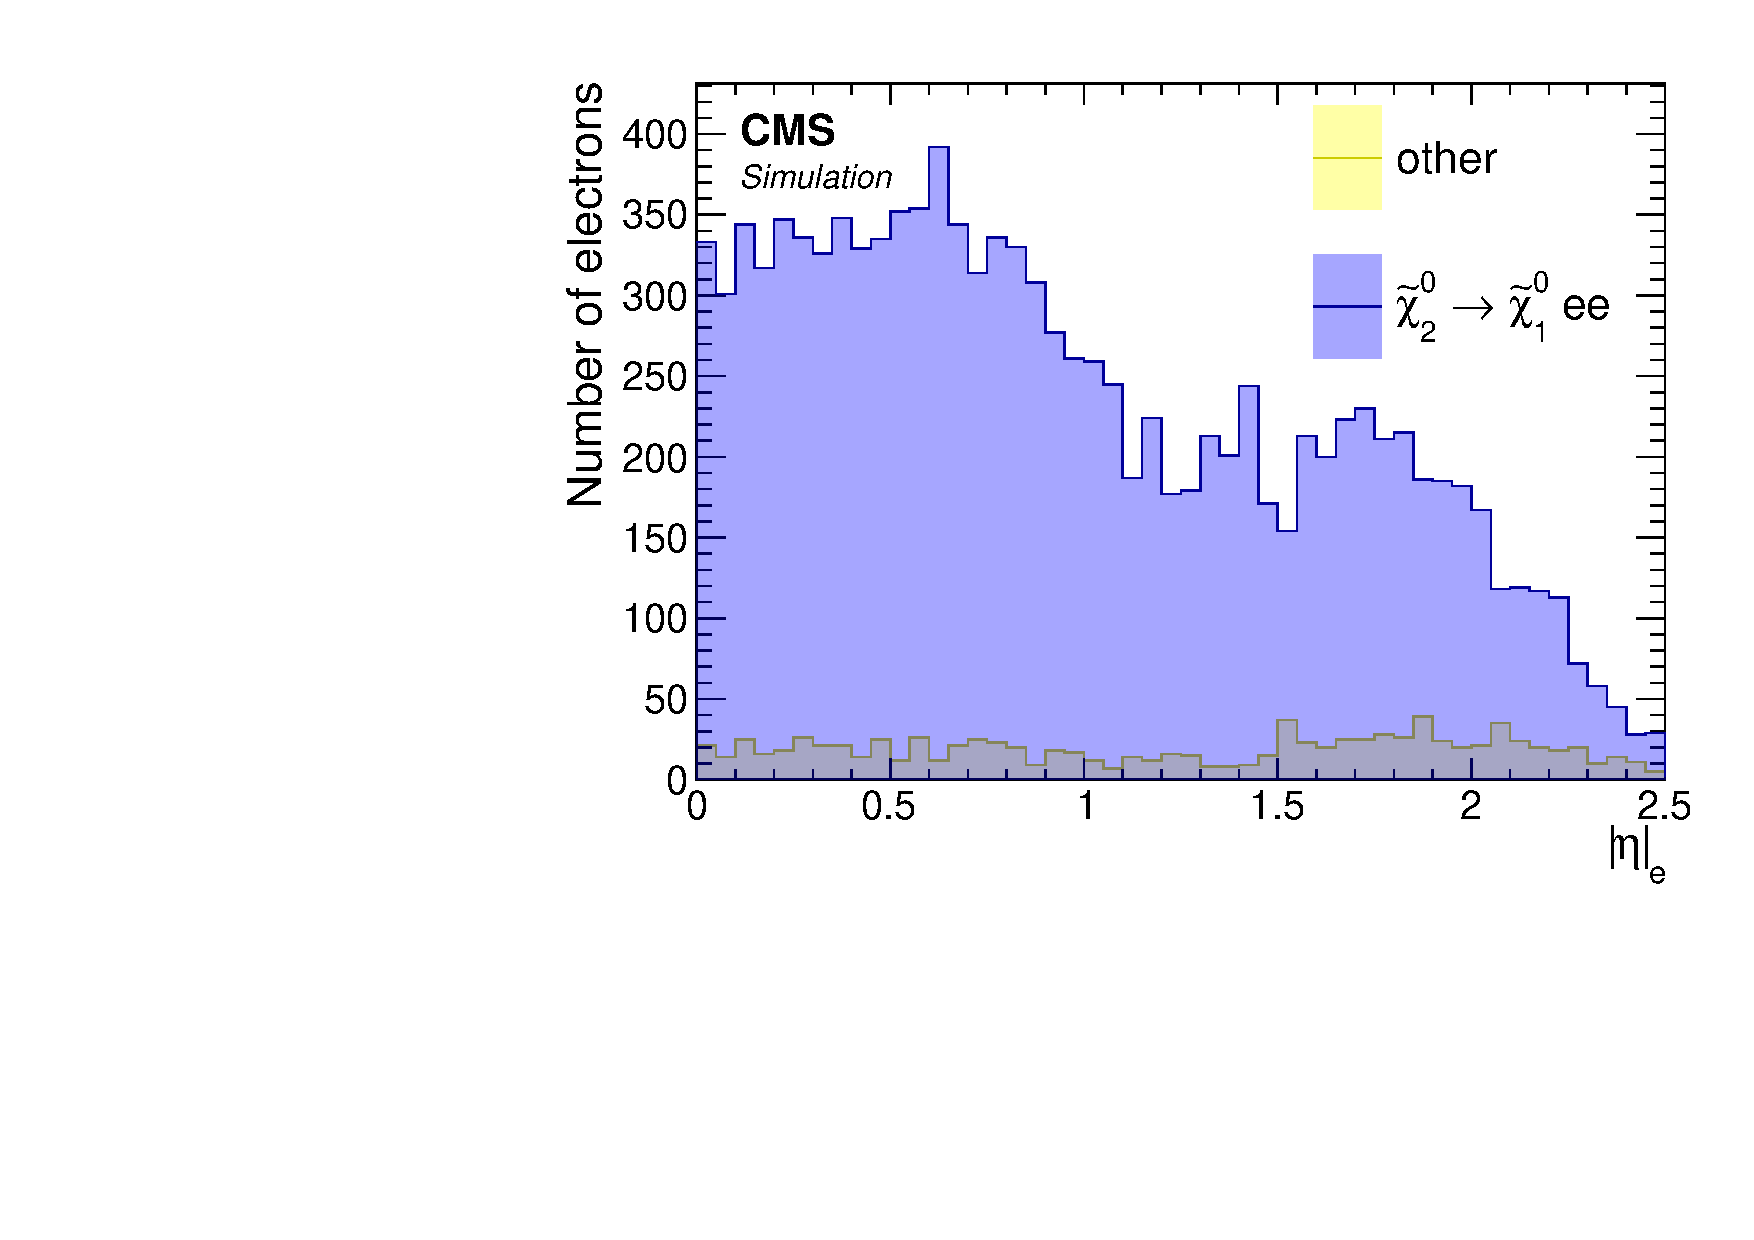
\includegraphics[width=0.48\linewidth]{plots/lepton_selection/lepton_selection_dm5p63/none_Electrons_eta_jet_iso.pdf} \,
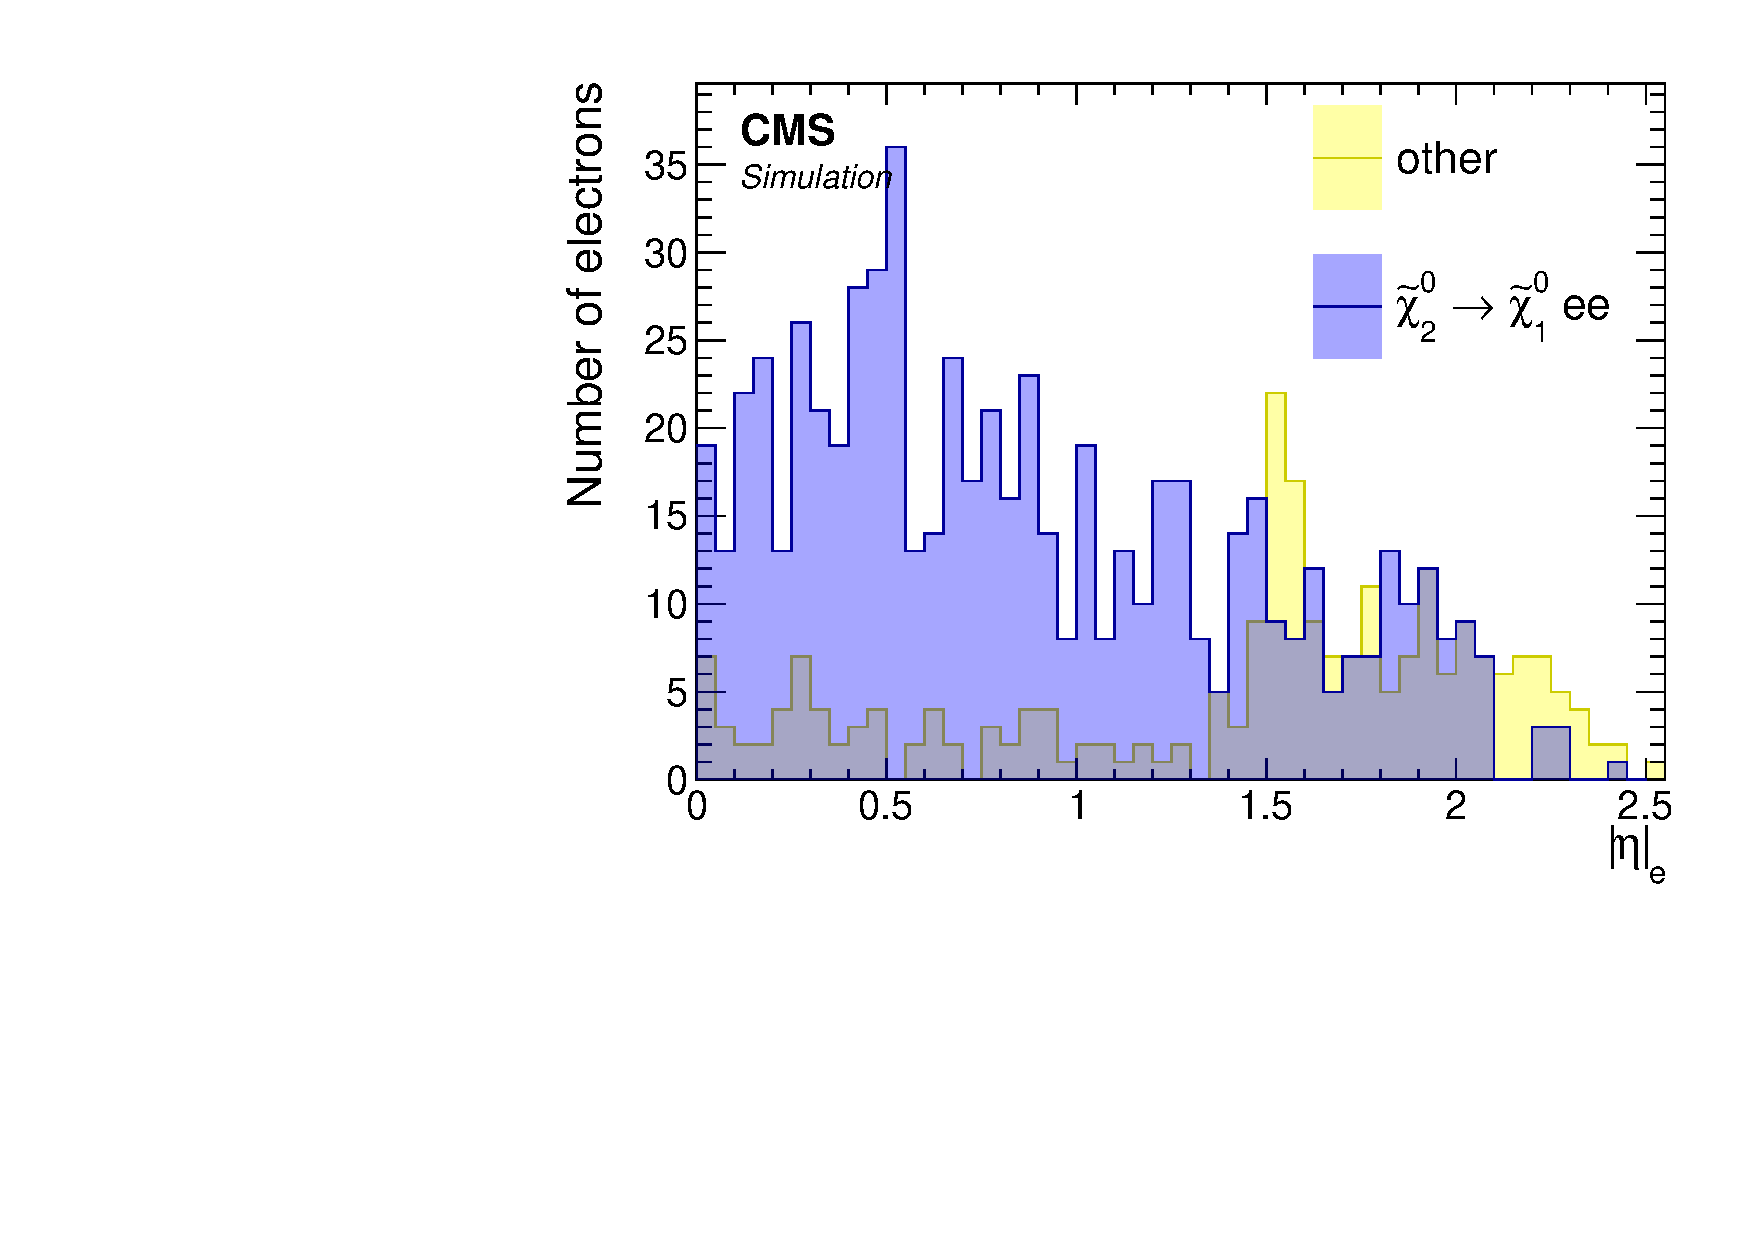
\includegraphics[width=0.48\linewidth]{plots/lepton_selection/lepton_selection_dm1p92/none_Electrons_eta_jet_iso.pdf}  \\
\caption[\abs{\eta} distribution of reconstructed electrons with loose ID passing jet-isolation]{ \abs{\eta} distribution of reconstructed electrons with loose ID passing jet-isolation for $\dm=5.63\GeV$ (left) and $\dm=1.92\GeV$ (right). Cuts of $\DR(\jmath_1,\Pe)>0.4$ and $\pt<15\GeV$ are applied.}
\label{fig:electrons-selection-eta-jet-iso}
\end{figure}

When we compare distributions~\ref{fig:electrons-selection-eta-jet-iso} with~\ref{fig:electrons-selection-eta}, we can see that our custom jet-isolation has done a good job purifying the electrons selection even further while being efficient in retaining the signal electrons.

%\subsubsection{Selection summary}

We summaries this section with the full selection of the analysis electrons:

\begin{itemize}[noitemsep]
\item $5<\pt<15\GeV$
\item $\abs{\eta} < 2.5$
\item $\DR(\jmath_1,\Pe)>0.4$
\item loose ID working point
\item pass jet-isolation
\end{itemize}

\subsection{Muons}
\label{sec:muon-selection}

In contrast to the electrons, we do not have an initial reconstruction \pt threshold of $5\GeV$. Therefore, we want to explore the possibility of lowering the \pt threshold as much as posible. This has been motivated in section~\ref{sec:muon-eta-pt}, where we saw that the lower \dm we want to probe, the lower \pt threshold we have to allow. Like in the electron case, the initial working point choice for reconstructed muon is loose (see~\ref{sec:reconstruction-and-identification}). We follow a similar procedure to the electrons case. The first distribution we look at in regards to the muons is their spatial separation from the leading jet in the event, $\DR(\jmath_1,\mu)$. We have seen in~\ref{fig:signal-pt-barrel-endcaps} that the muon endcaps are capable of reconstructing muons with $\pt<3\GeV$ while the barrel cannot. It therefore makes sense to look at a split view of barrel and endcaps for the following distributions.

\begin{figure}[!htb]
\centering
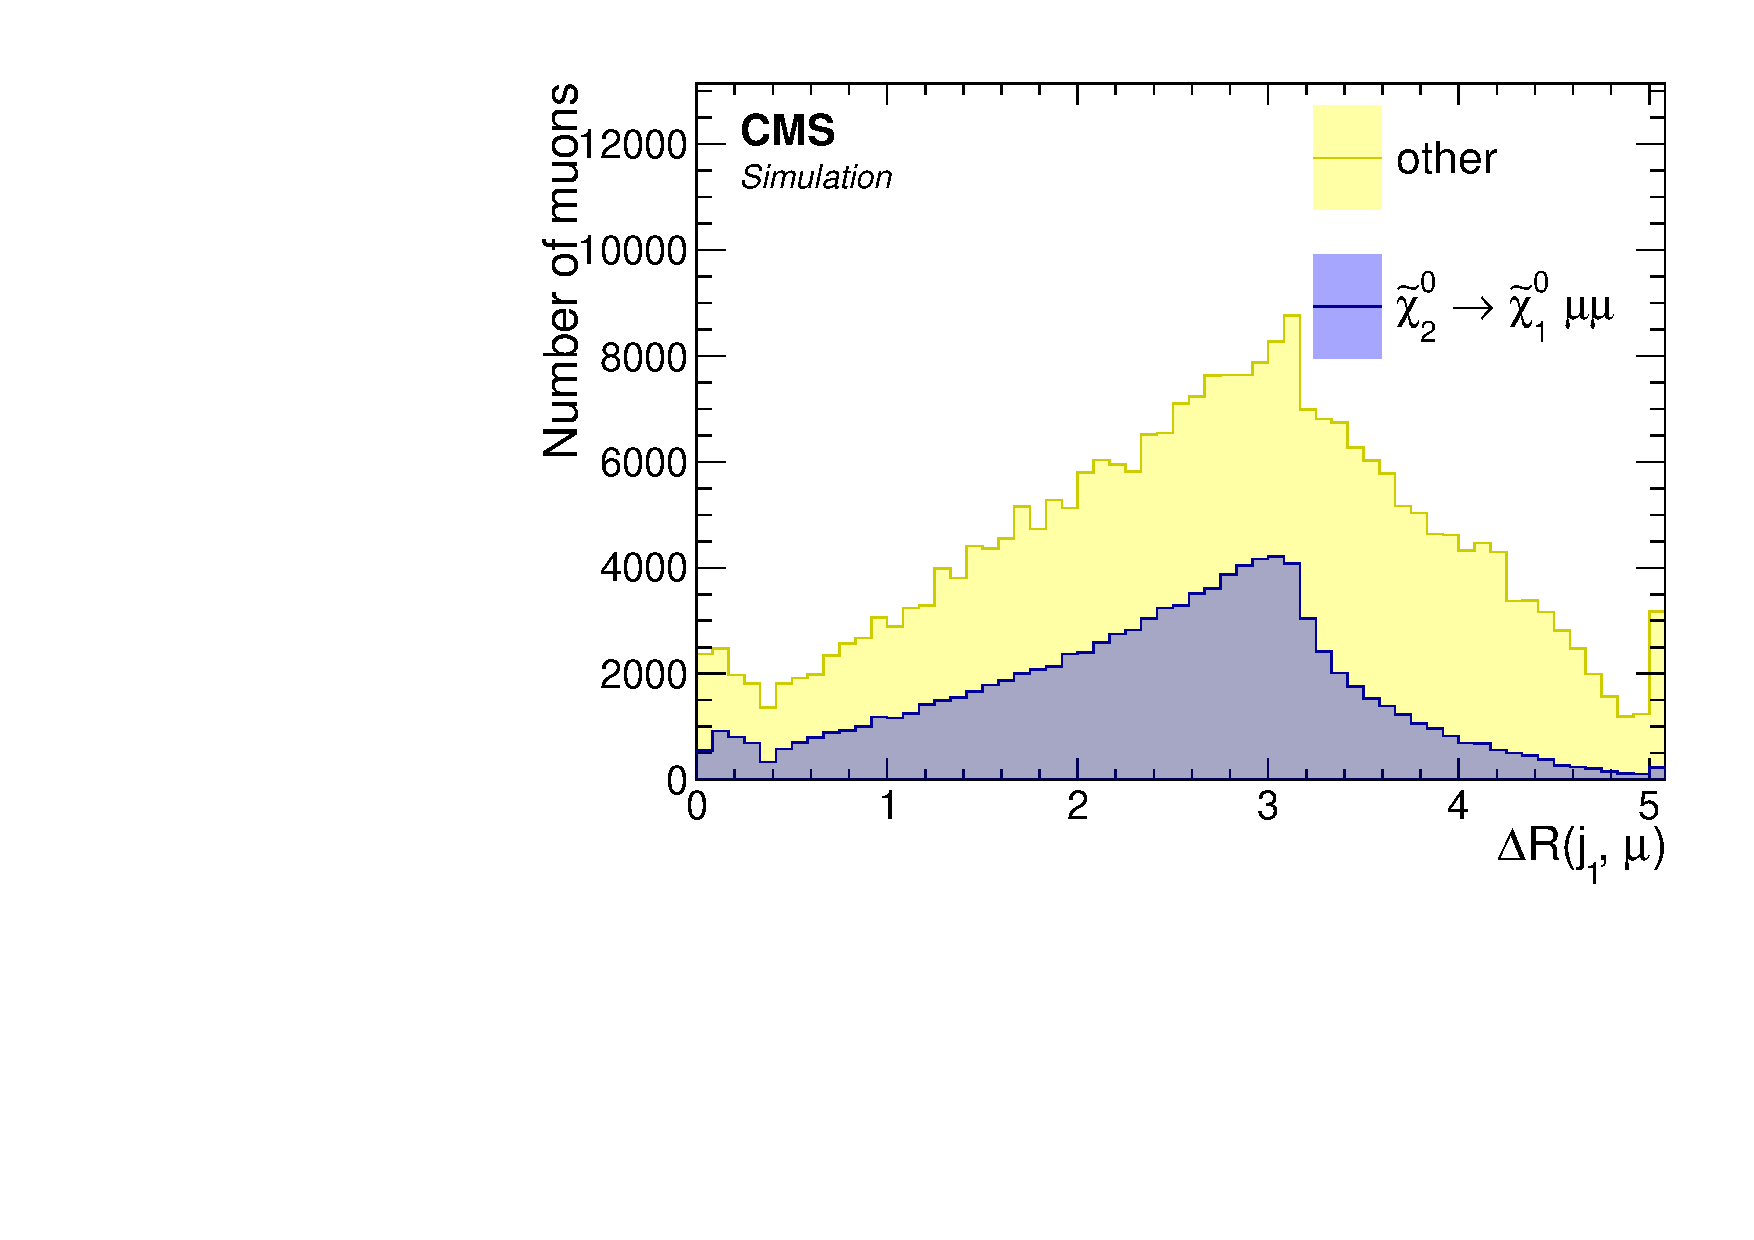
\includegraphics[width=0.32\linewidth]{plots/lepton_selection/lepton_selection_dm5p63/none_Muons_rlj.pdf} \,
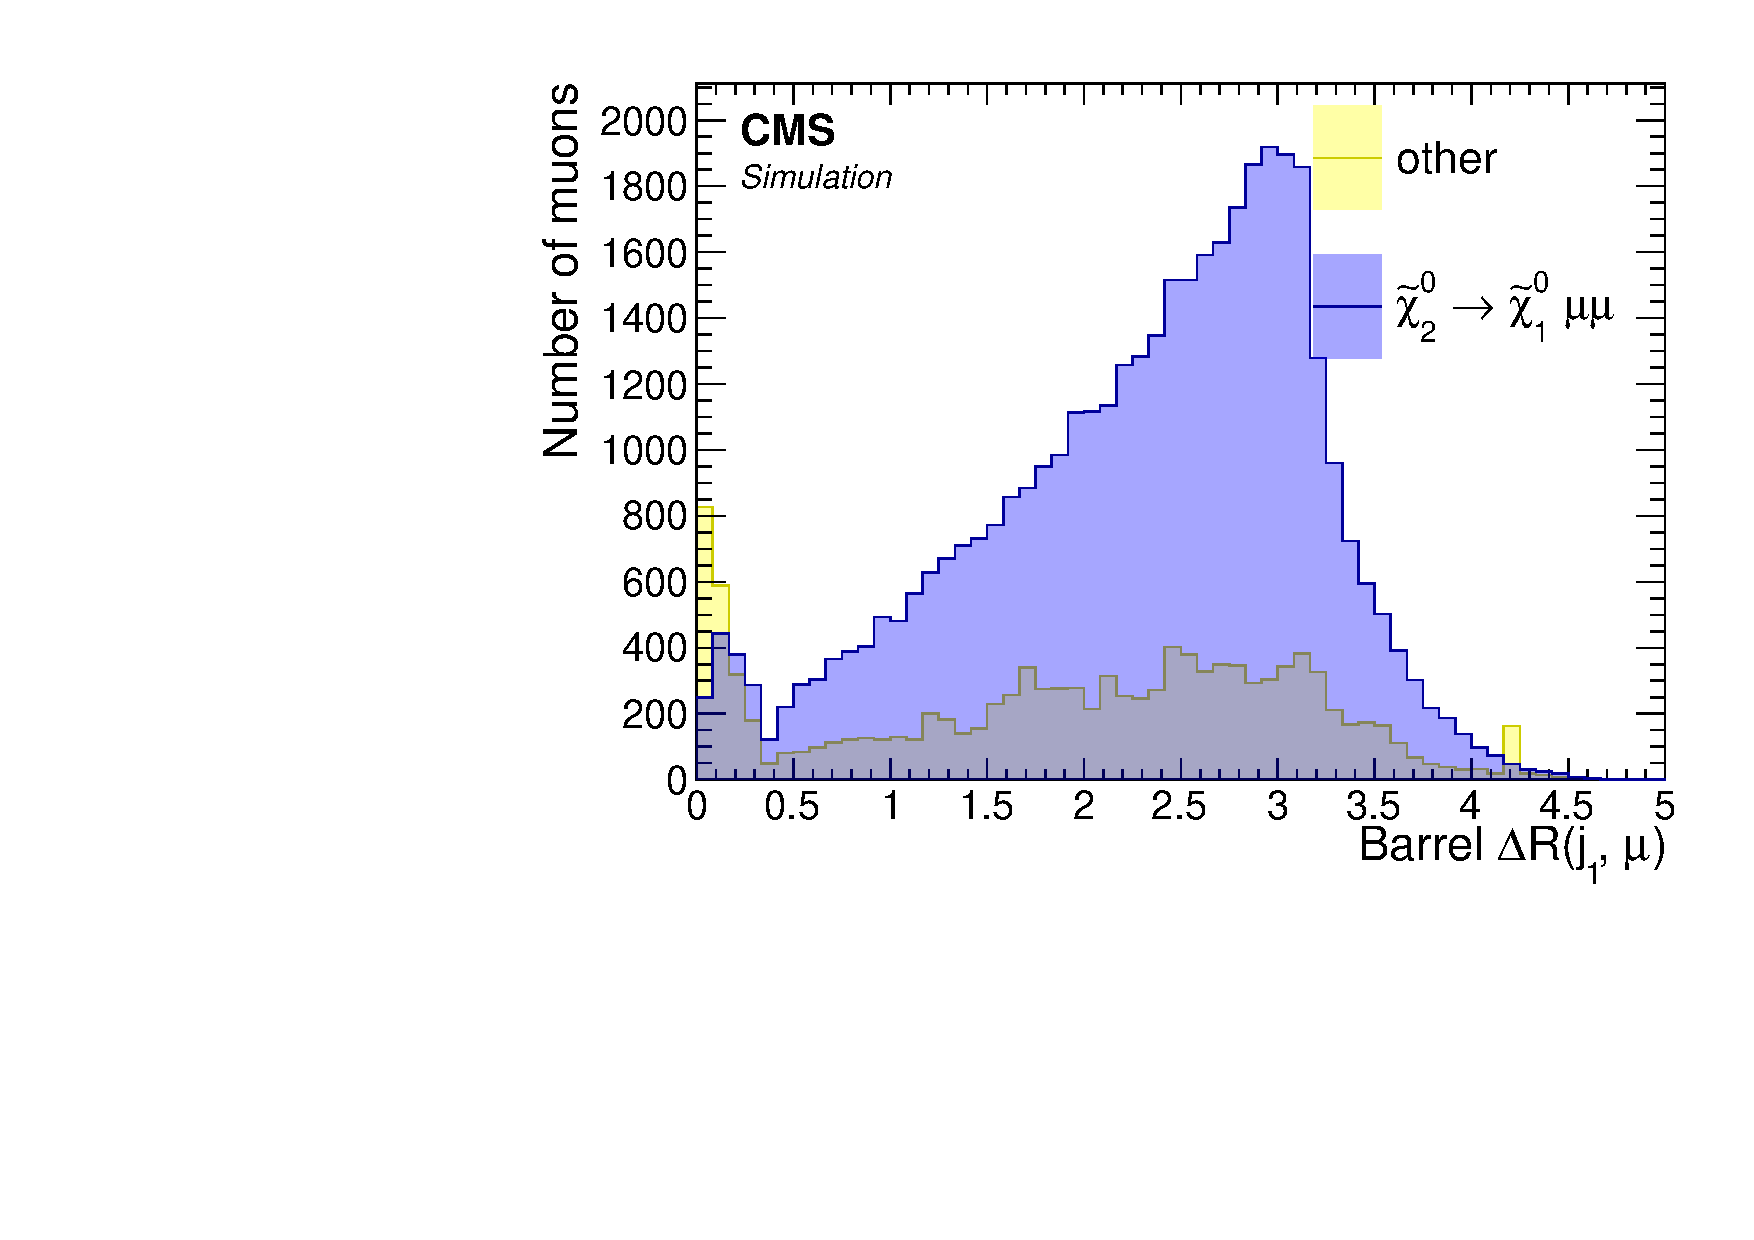
\includegraphics[width=0.32\linewidth]{plots/lepton_selection/lepton_selection_dm5p63/none_Muons_rlj_barrel.pdf}
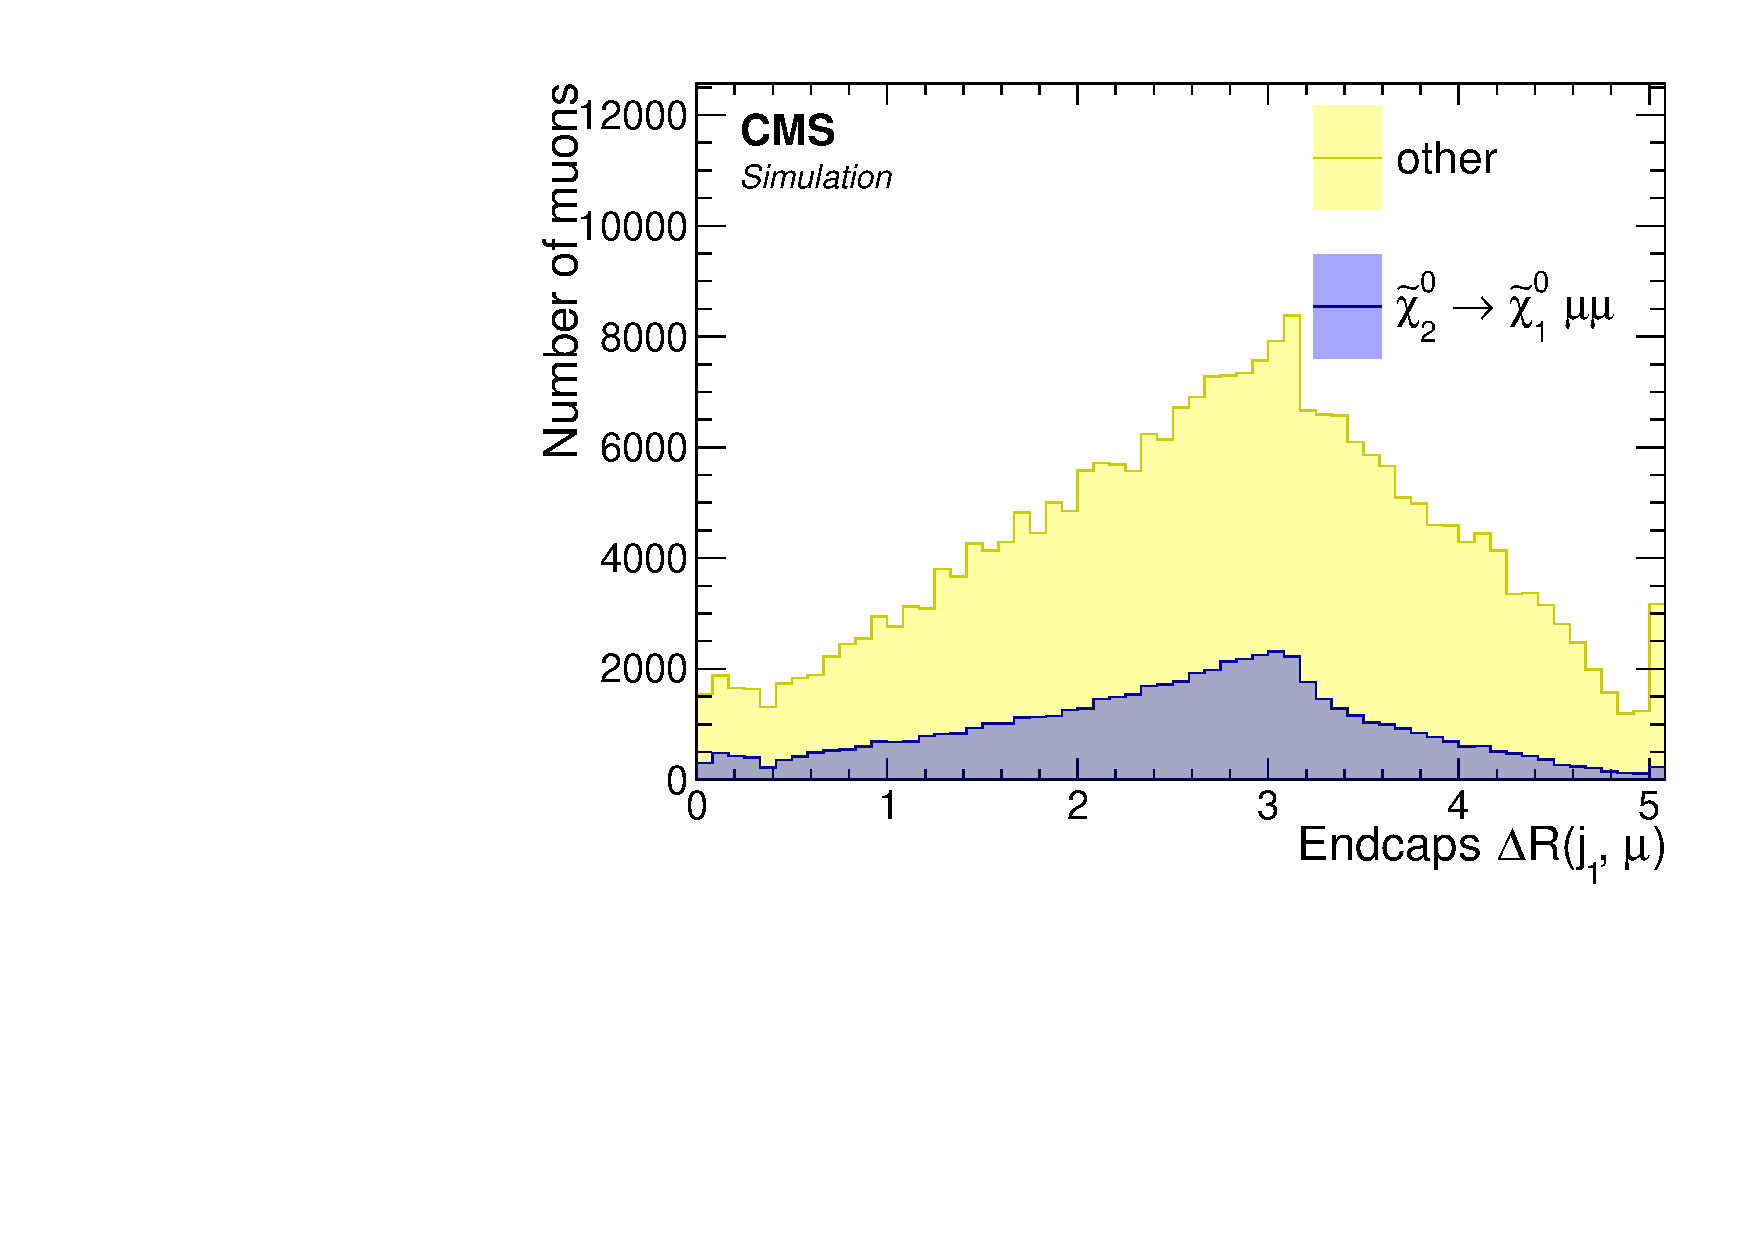
\includegraphics[width=0.32\linewidth]{plots/lepton_selection/lepton_selection_dm5p63/none_Muons_rlj_endcape.pdf}  \\
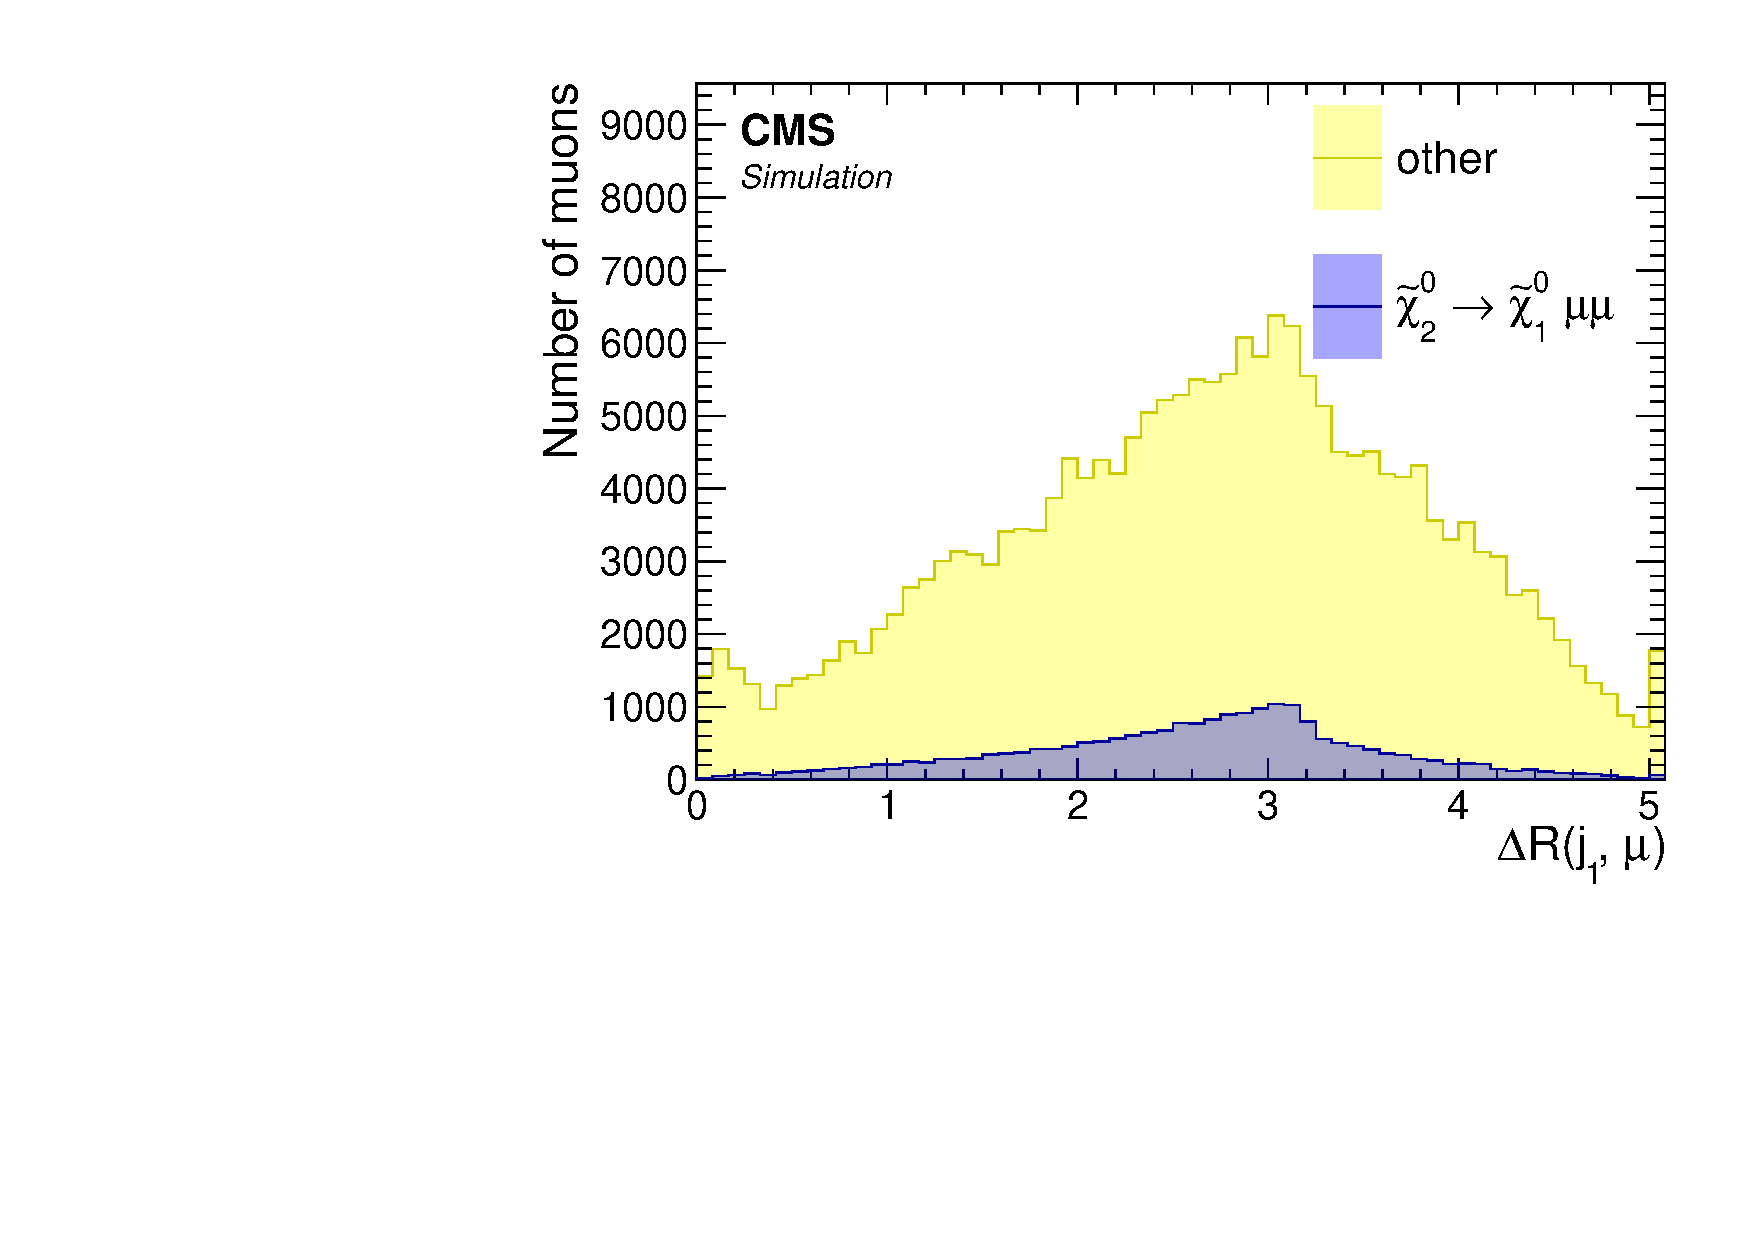
\includegraphics[width=0.32\linewidth]{plots/lepton_selection/lepton_selection_dm1p92/none_Muons_rlj.pdf} \,
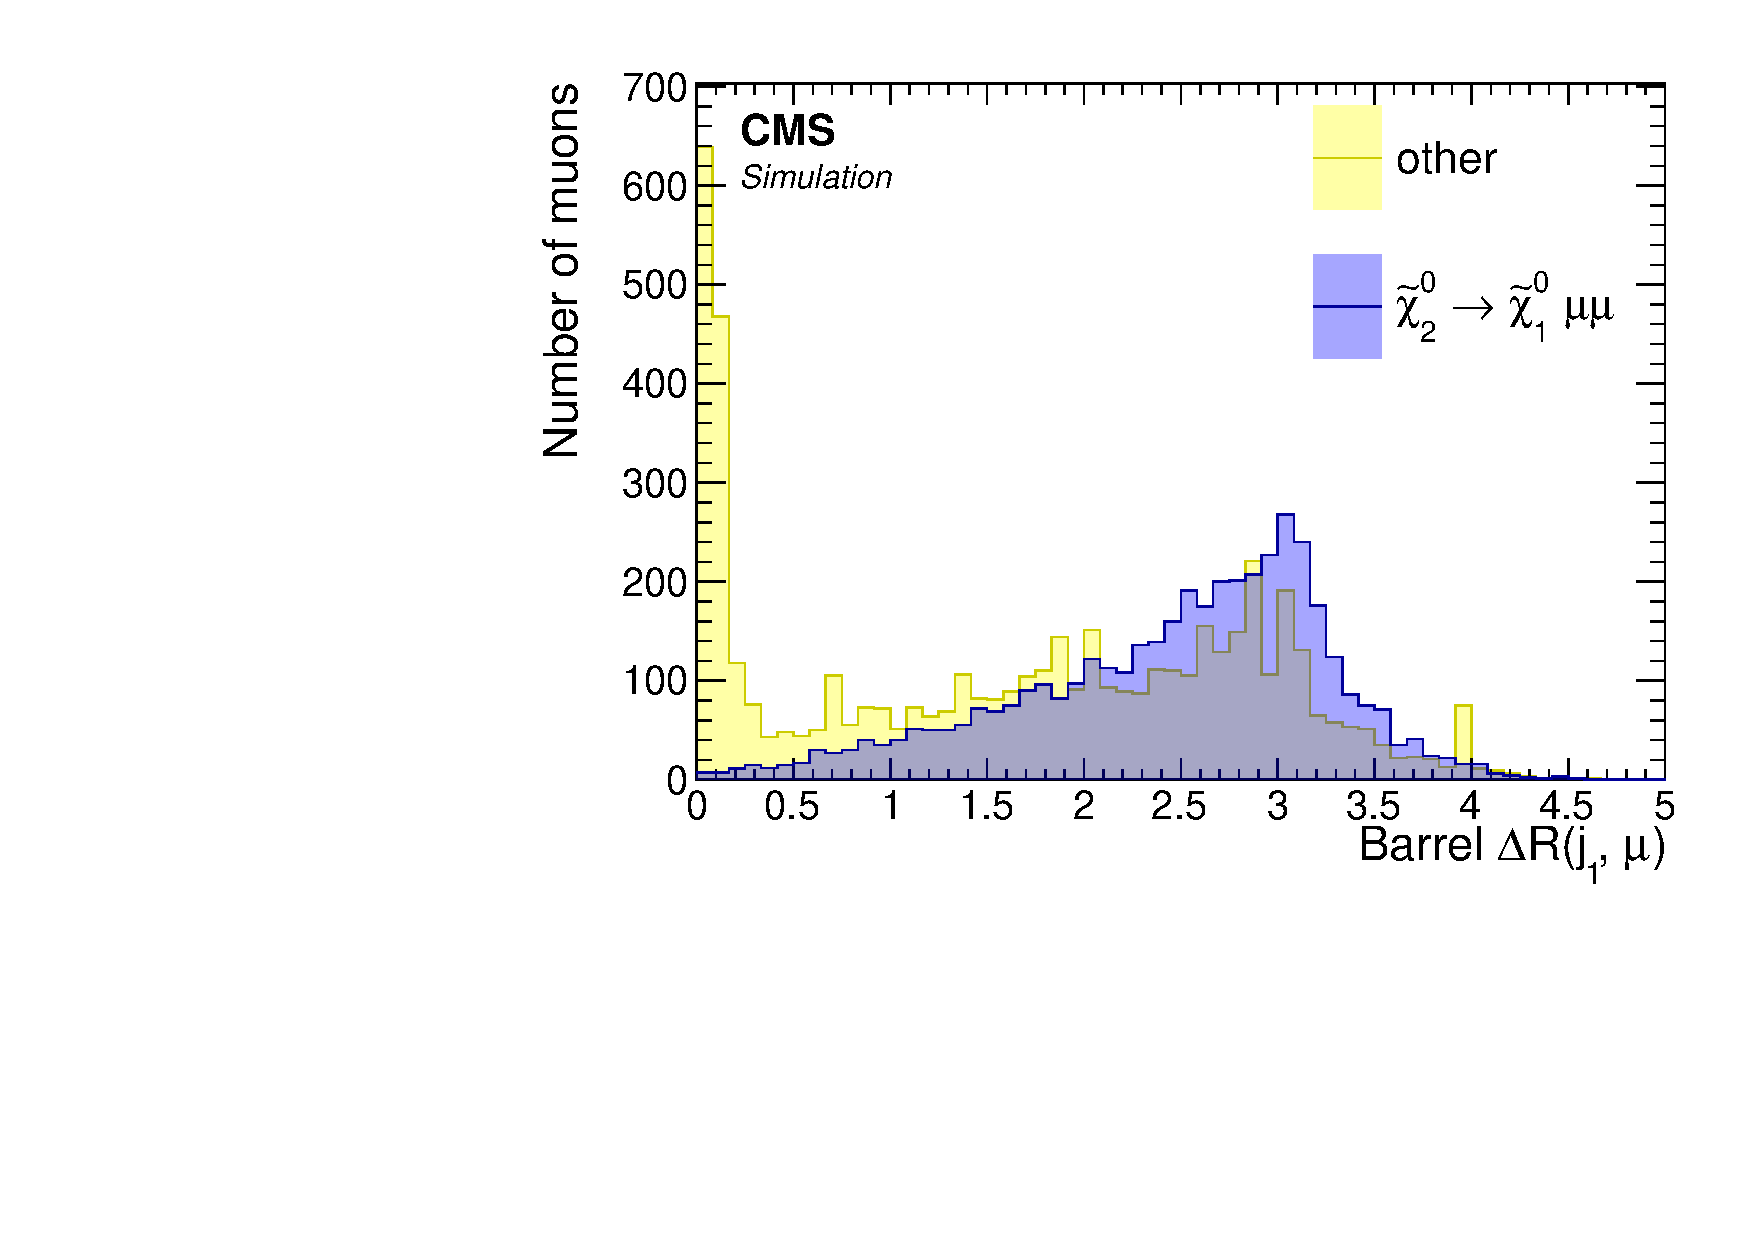
\includegraphics[width=0.32\linewidth]{plots/lepton_selection/lepton_selection_dm1p92/none_Muons_rlj_barrel.pdf}
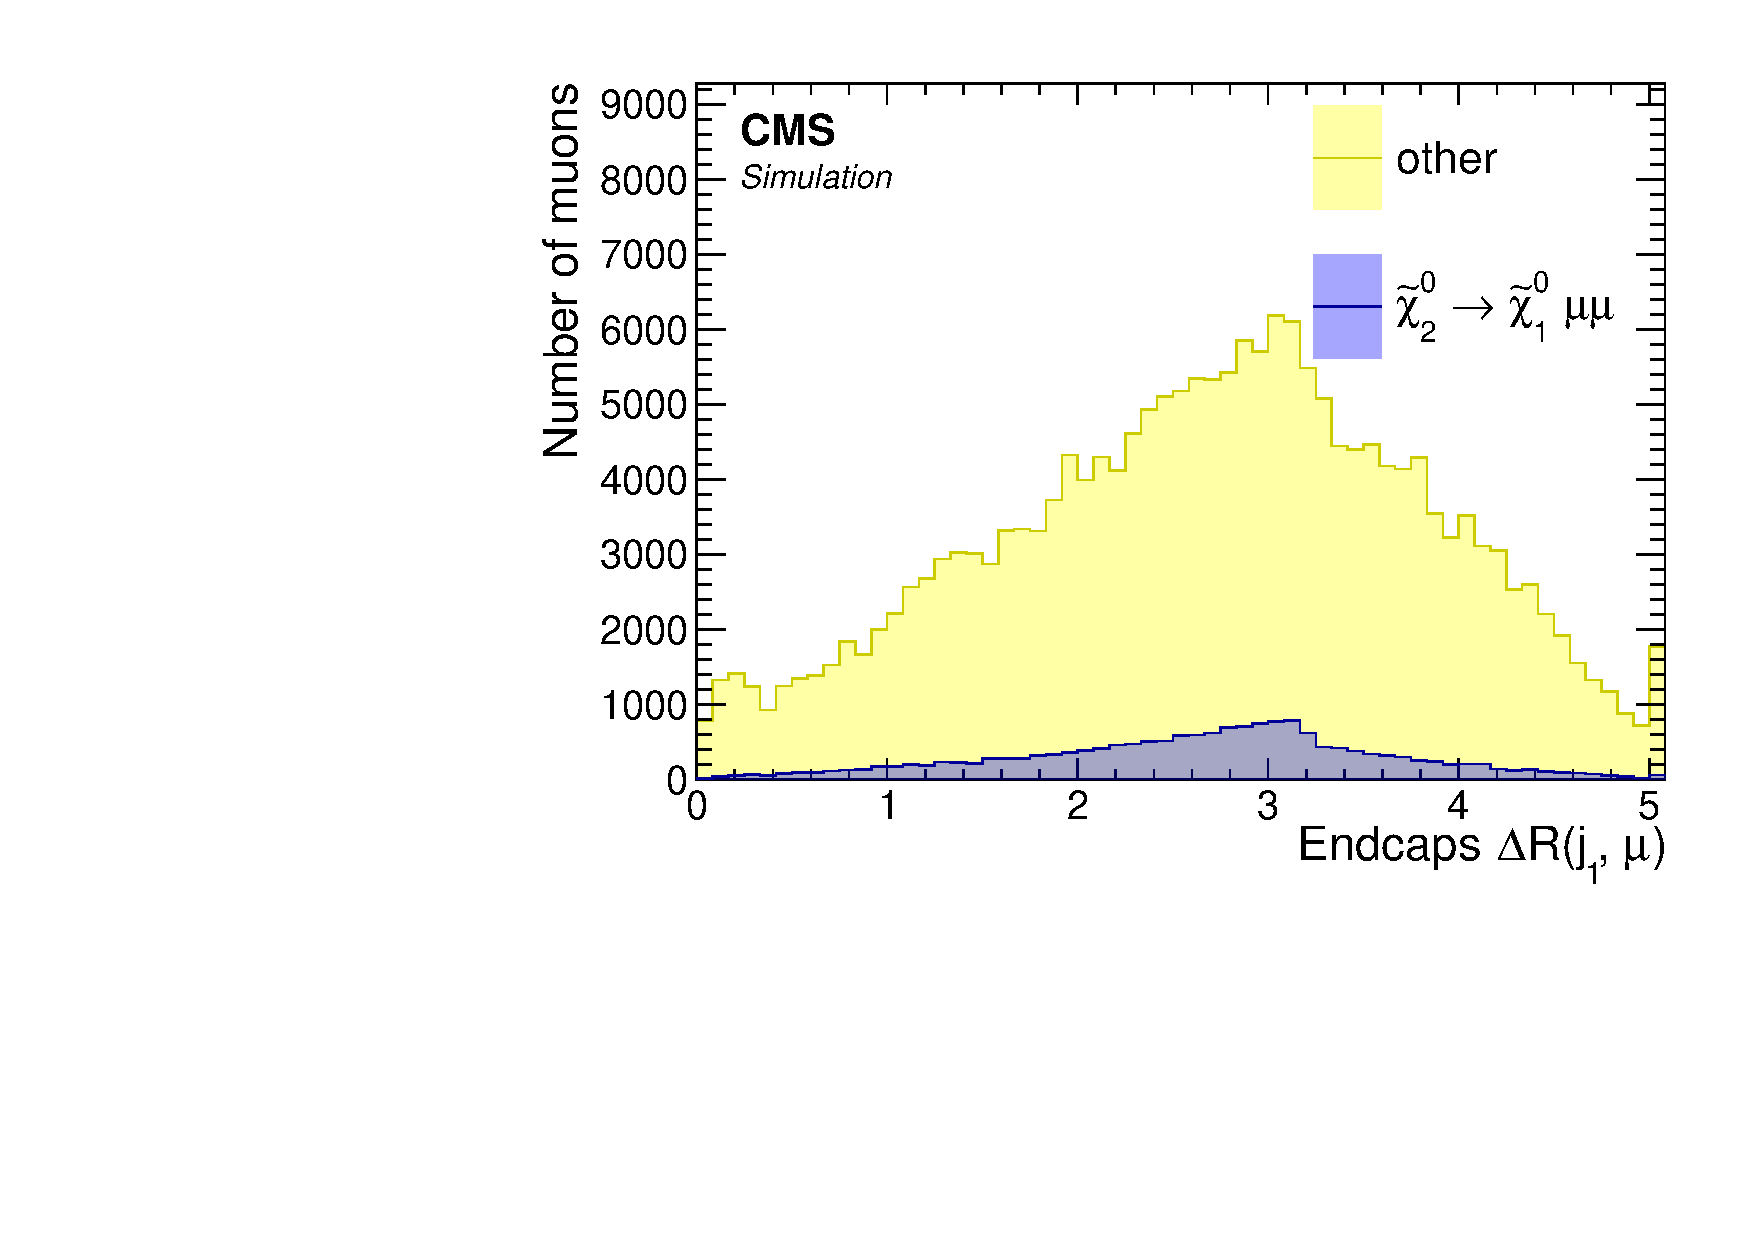
\includegraphics[width=0.32\linewidth]{plots/lepton_selection/lepton_selection_dm1p92/none_Muons_rlj_endcape.pdf}  \\
\caption[Spatial seperation between reconstructed muons and the leading jet $\DR(\jmath_1,\mu)$]{Spatial seperation between reconstructed muons with loose ID and the leading jet $\DR(\jmath_1,\mu)$ for $\dm=5.63\GeV$ (top) and $\dm=1.92\GeV$ (bottom) in the inclusive case (left), barrel (middle) and endcaps (right).}
\label{fig:muons-dr-lj}
\end{figure}

Since the muons in the endcaps has lower \pt than the muons in the barrel, which is able to reconstruct muons with $\pt>3\GeV$ only, the purity in the endcaps is much lower than the purity in the barrel, and the selection we are constructing here attempts to purify the muons further. Just as in the electrons case, we select muons with $\DR(\jmath_1,\mu)>0.4$, and that selection will apply for the rest of the section.

Next we turn into the \gls{pt} distributions. We apply the previous cut of $\DR(\jmath_1,\mu)>0.4$. As we've already seen in~\ref{sec:muon-eta-pt}, the \gls{pt} and in the electron case, the \pt distribution depends strongly on \gls{dm}, and we try to favor the low \gls{dm} acceptance in order to be more sensitive to it. The \pt distributions we see in~\ref{fig:muons-selectrion-pt} suggest a cut identical to the electron case of $\pt<15\GeV$. It is worth mentioning that the \pt of the muons are fed into the training of the \gls{bdt} for further refinement, and therefore the exact value is being determined here quite loosely. The actual maximum value of the \pt of the muons will depend on the \gls{bdt} cut being used to define the signal region.

\begin{figure}[!htb]
\centering
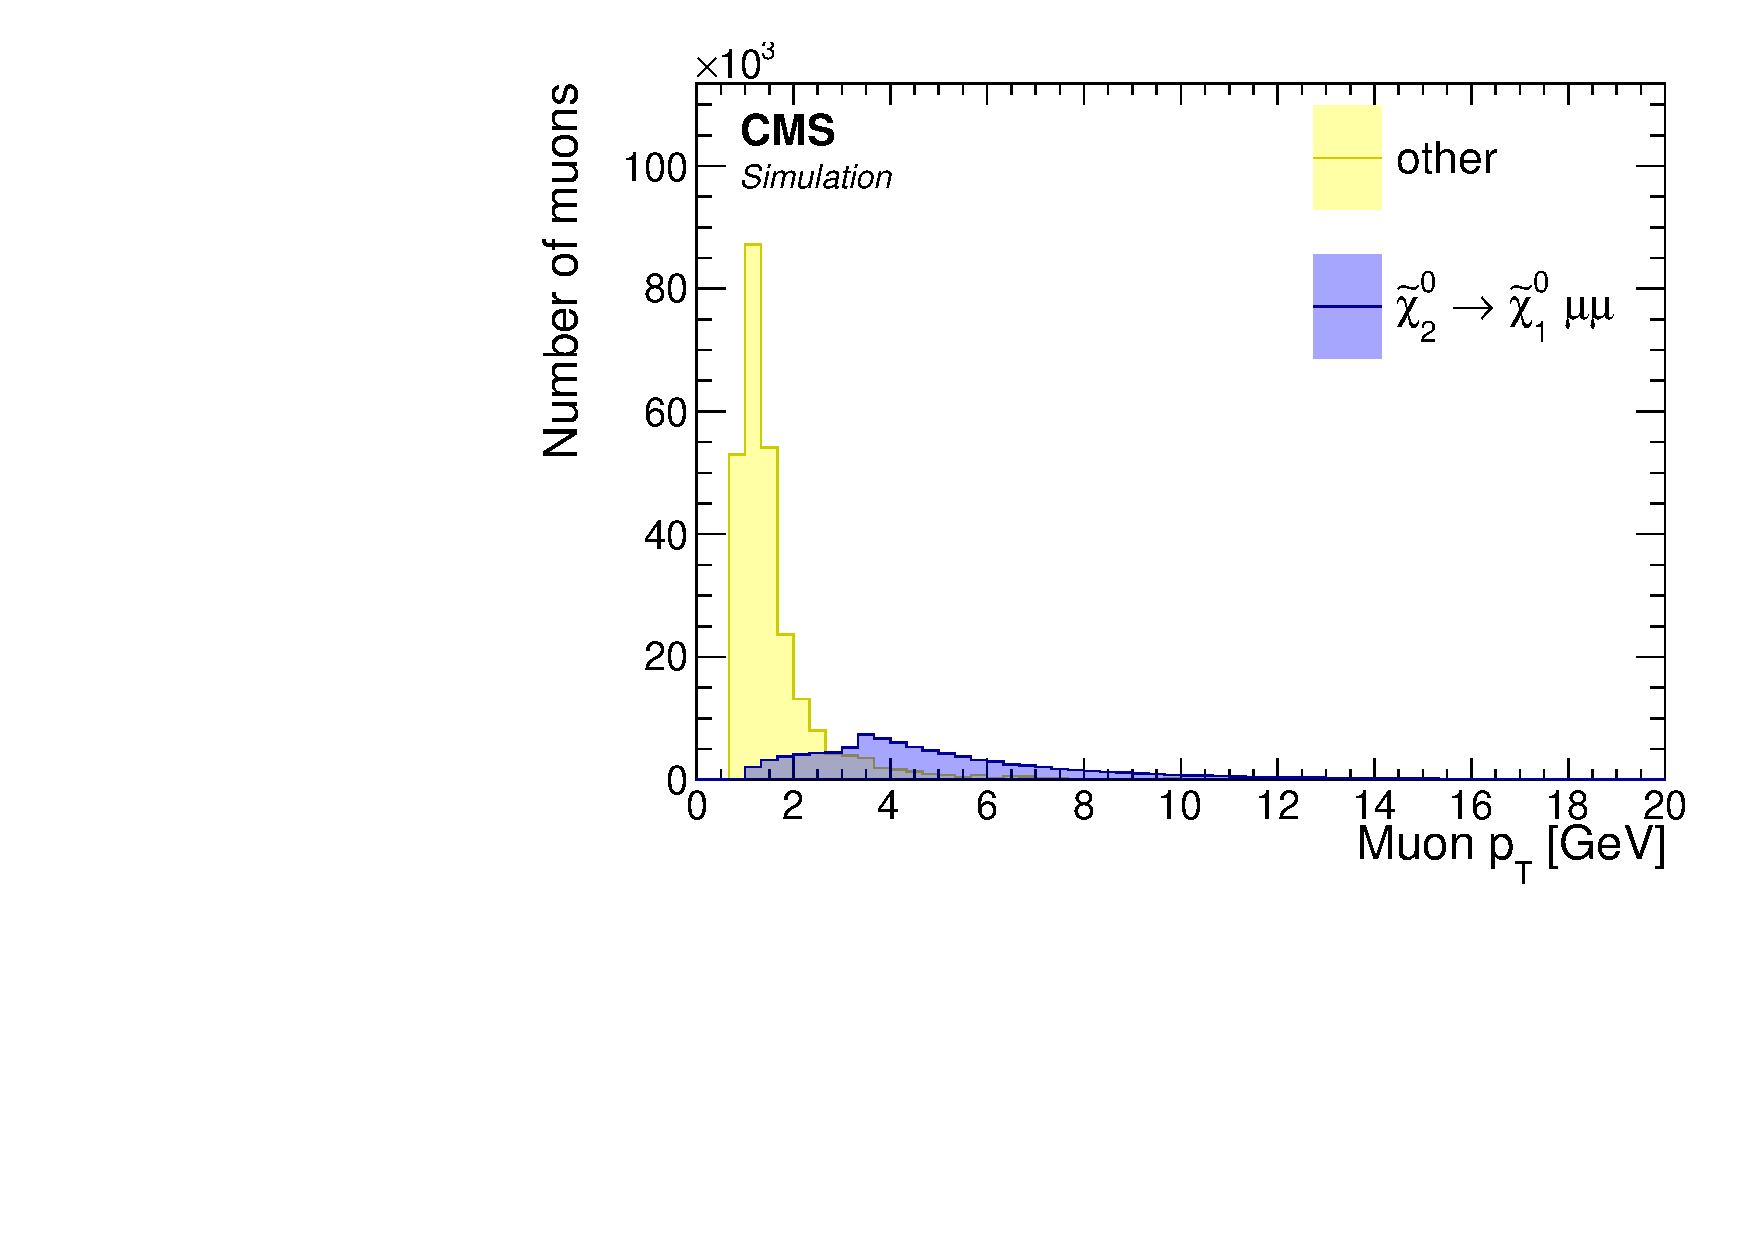
\includegraphics[width=0.32\linewidth]{plots/lepton_selection/lepton_selection_dm5p63/none_Muons_pt.pdf} \,
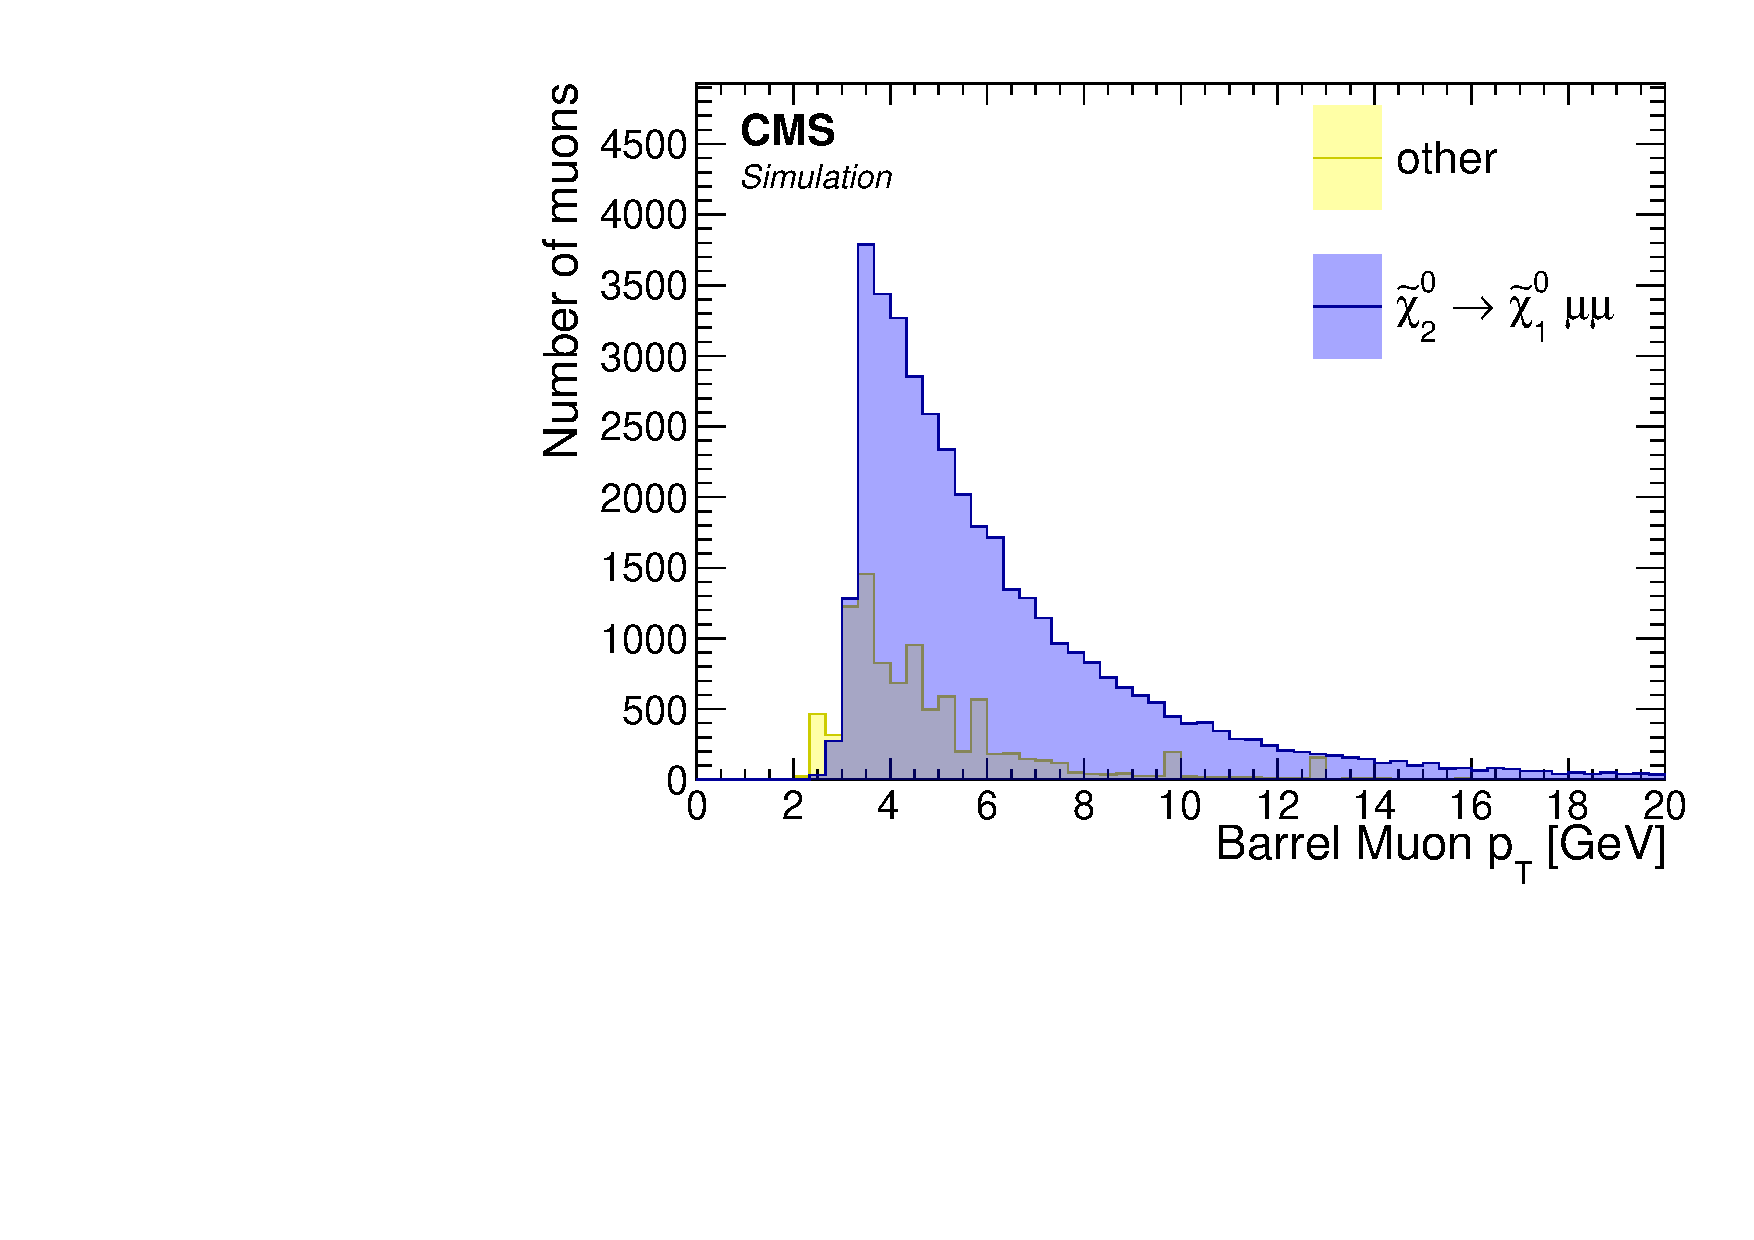
\includegraphics[width=0.32\linewidth]{plots/lepton_selection/lepton_selection_dm5p63/none_Muons_pt_barrel.pdf}
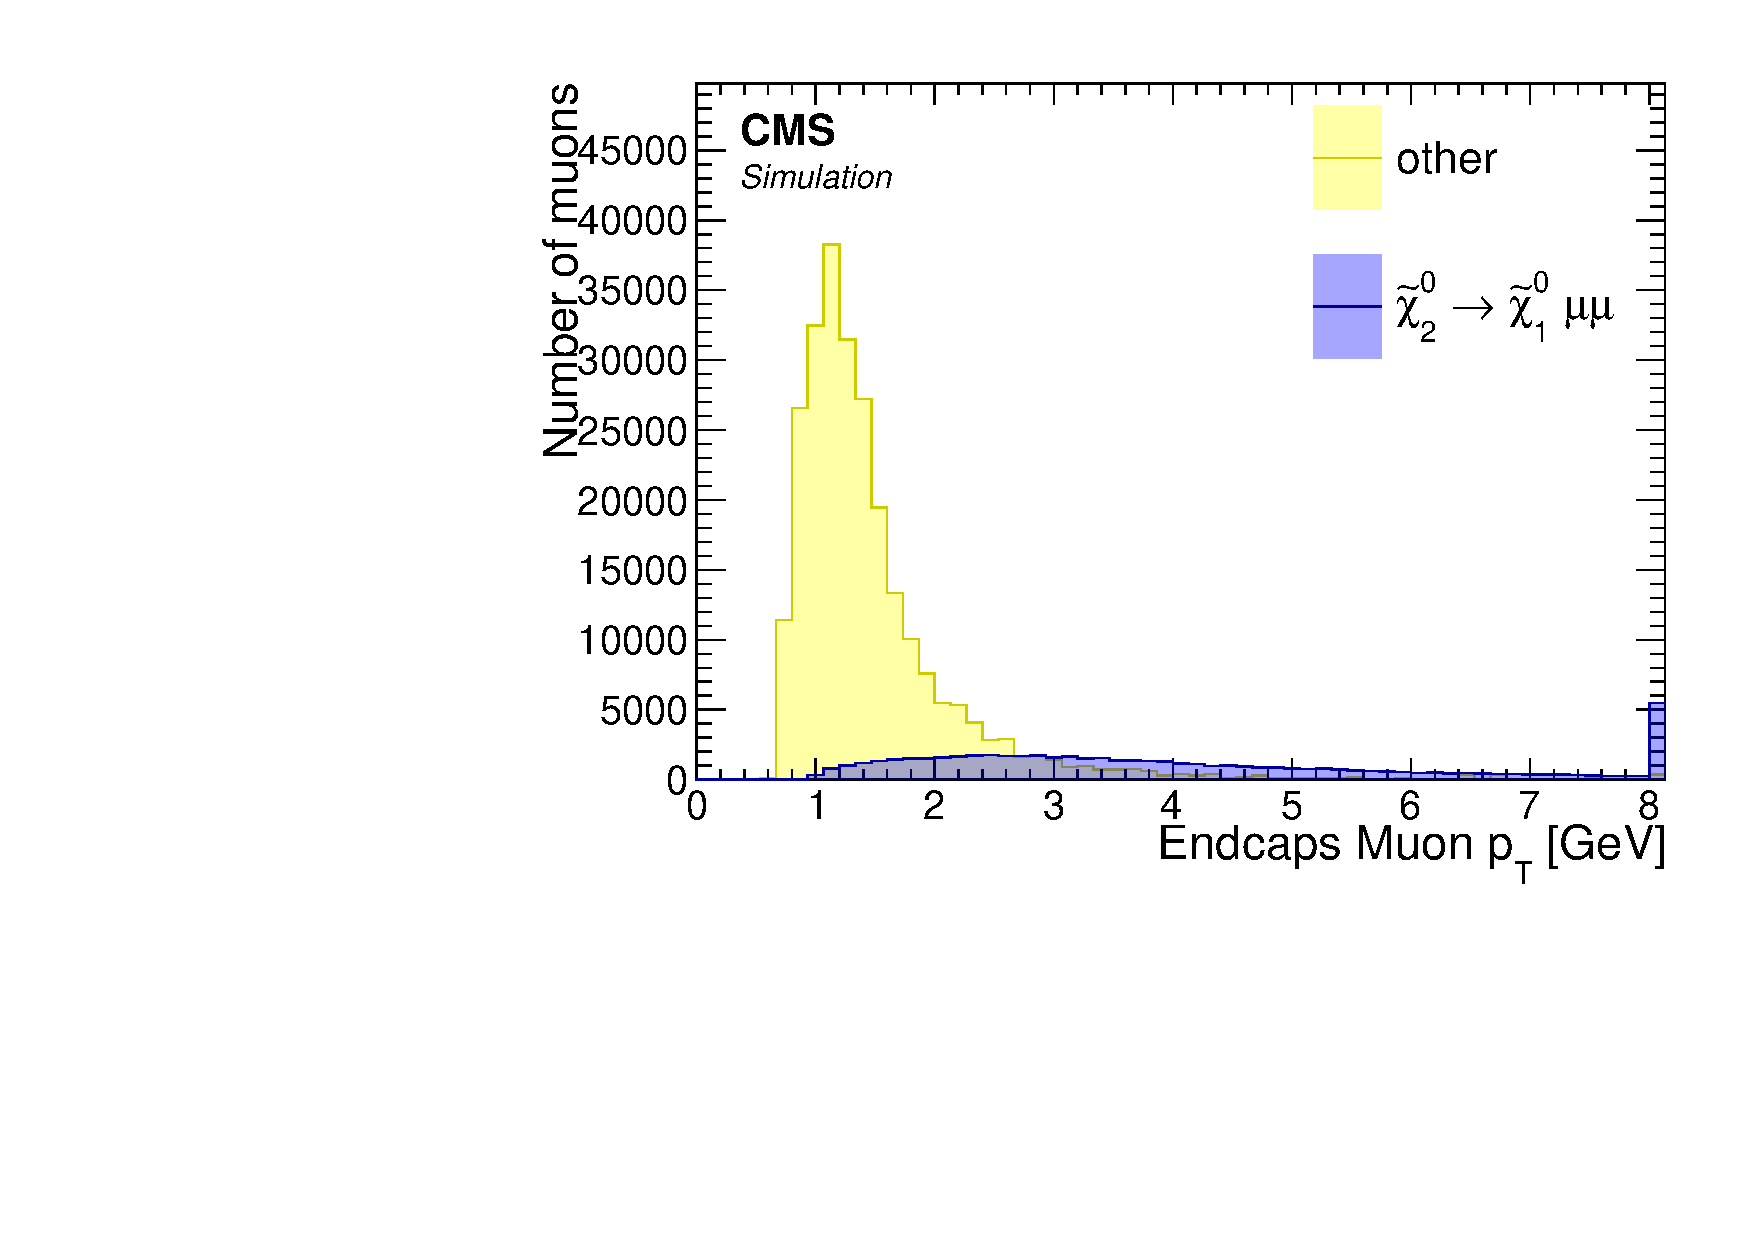
\includegraphics[width=0.32\linewidth]{plots/lepton_selection/lepton_selection_dm5p63/none_Muons_pt_endcape.pdf}  \\
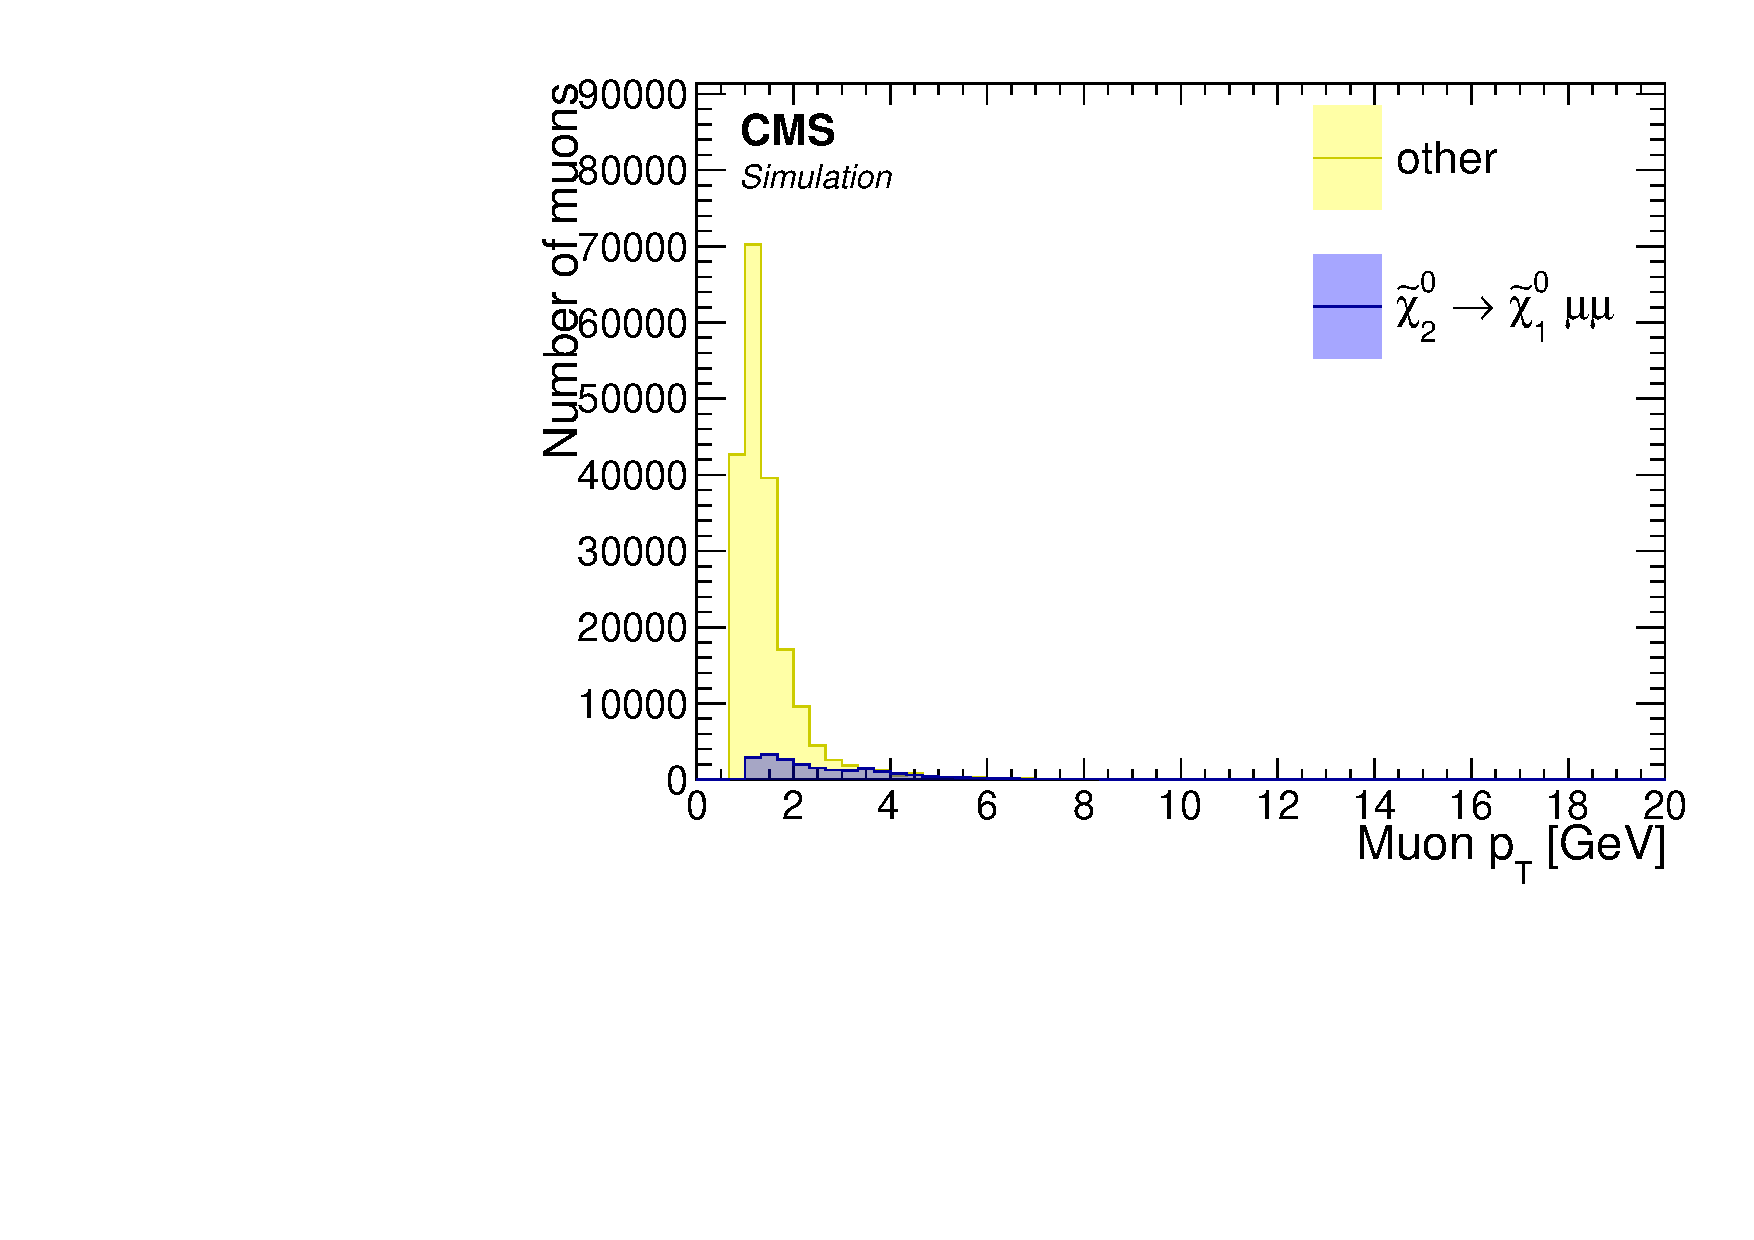
\includegraphics[width=0.32\linewidth]{plots/lepton_selection/lepton_selection_dm1p92/none_Muons_pt.pdf} \,
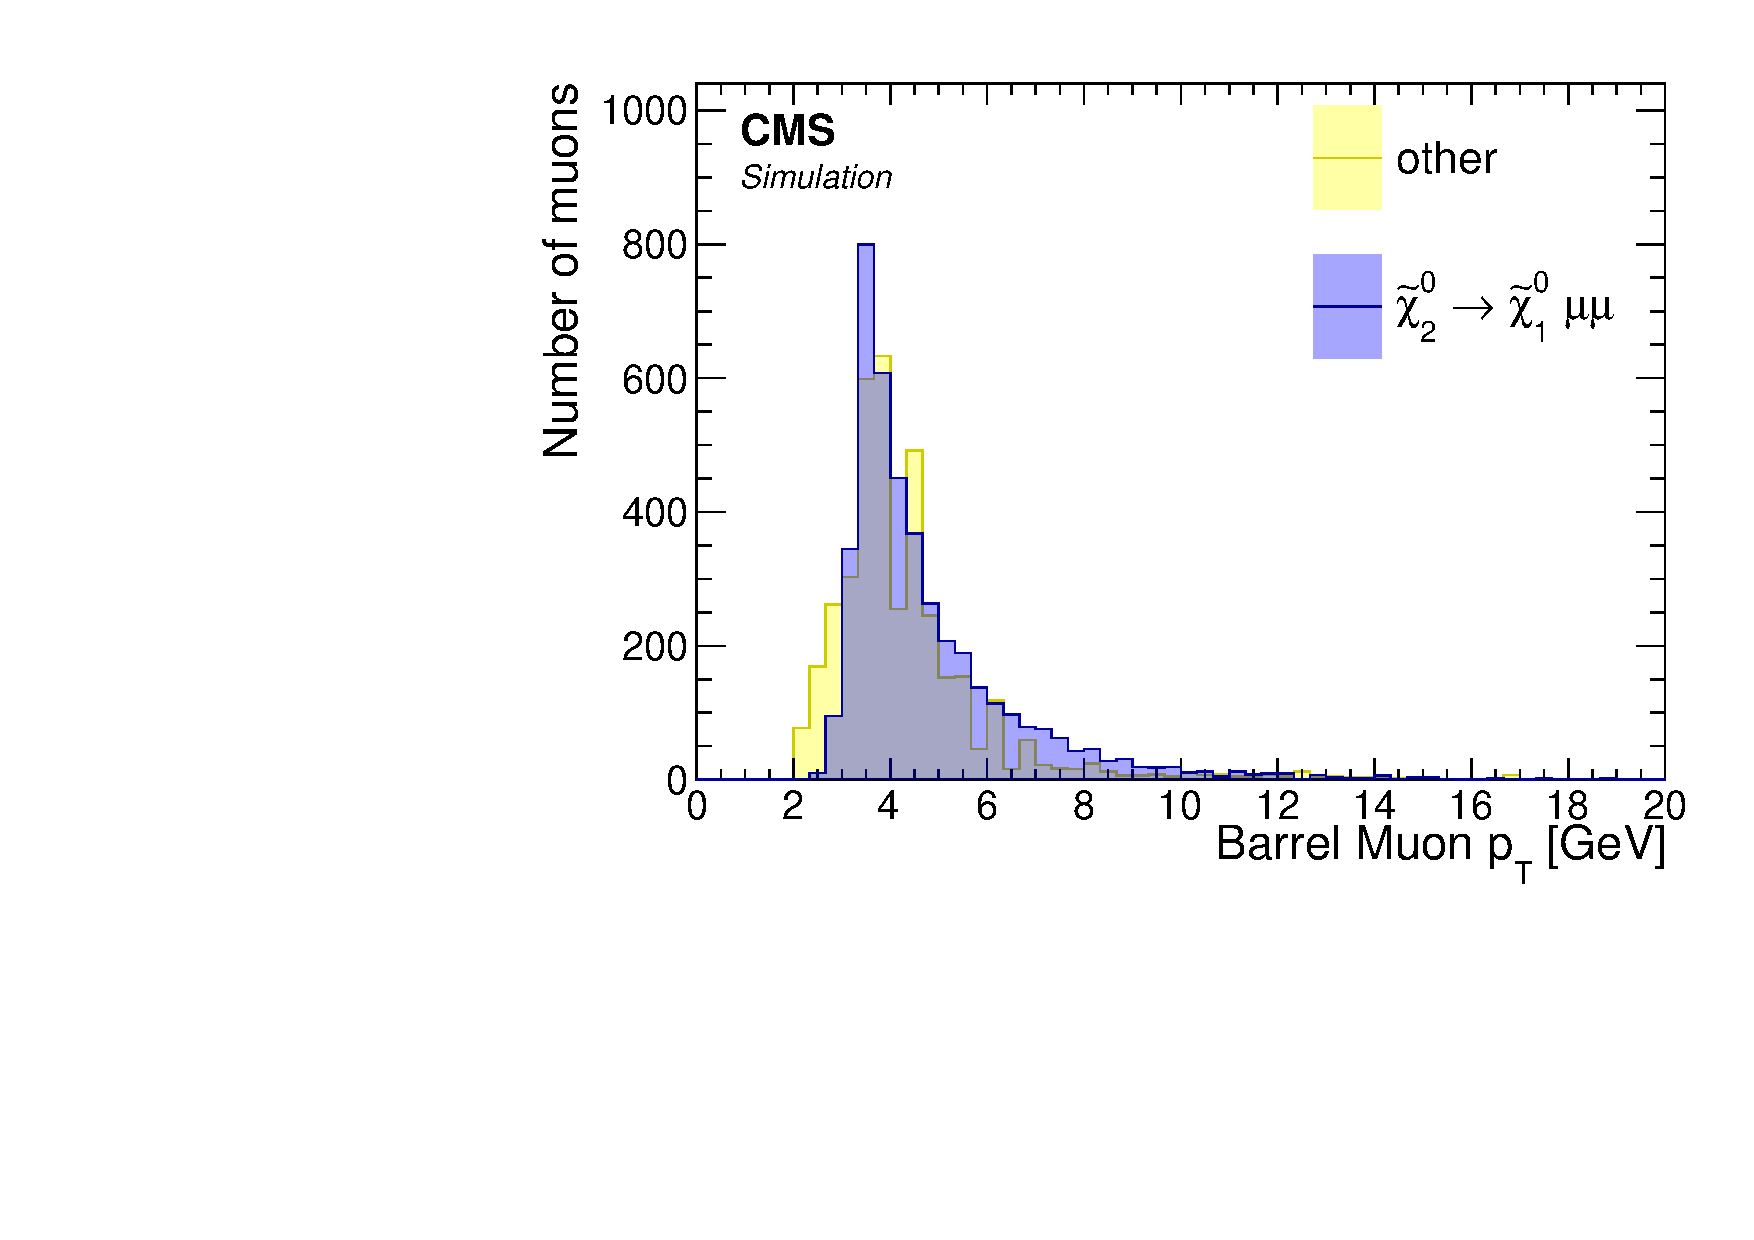
\includegraphics[width=0.32\linewidth]{plots/lepton_selection/lepton_selection_dm1p92/none_Muons_pt_barrel.pdf}
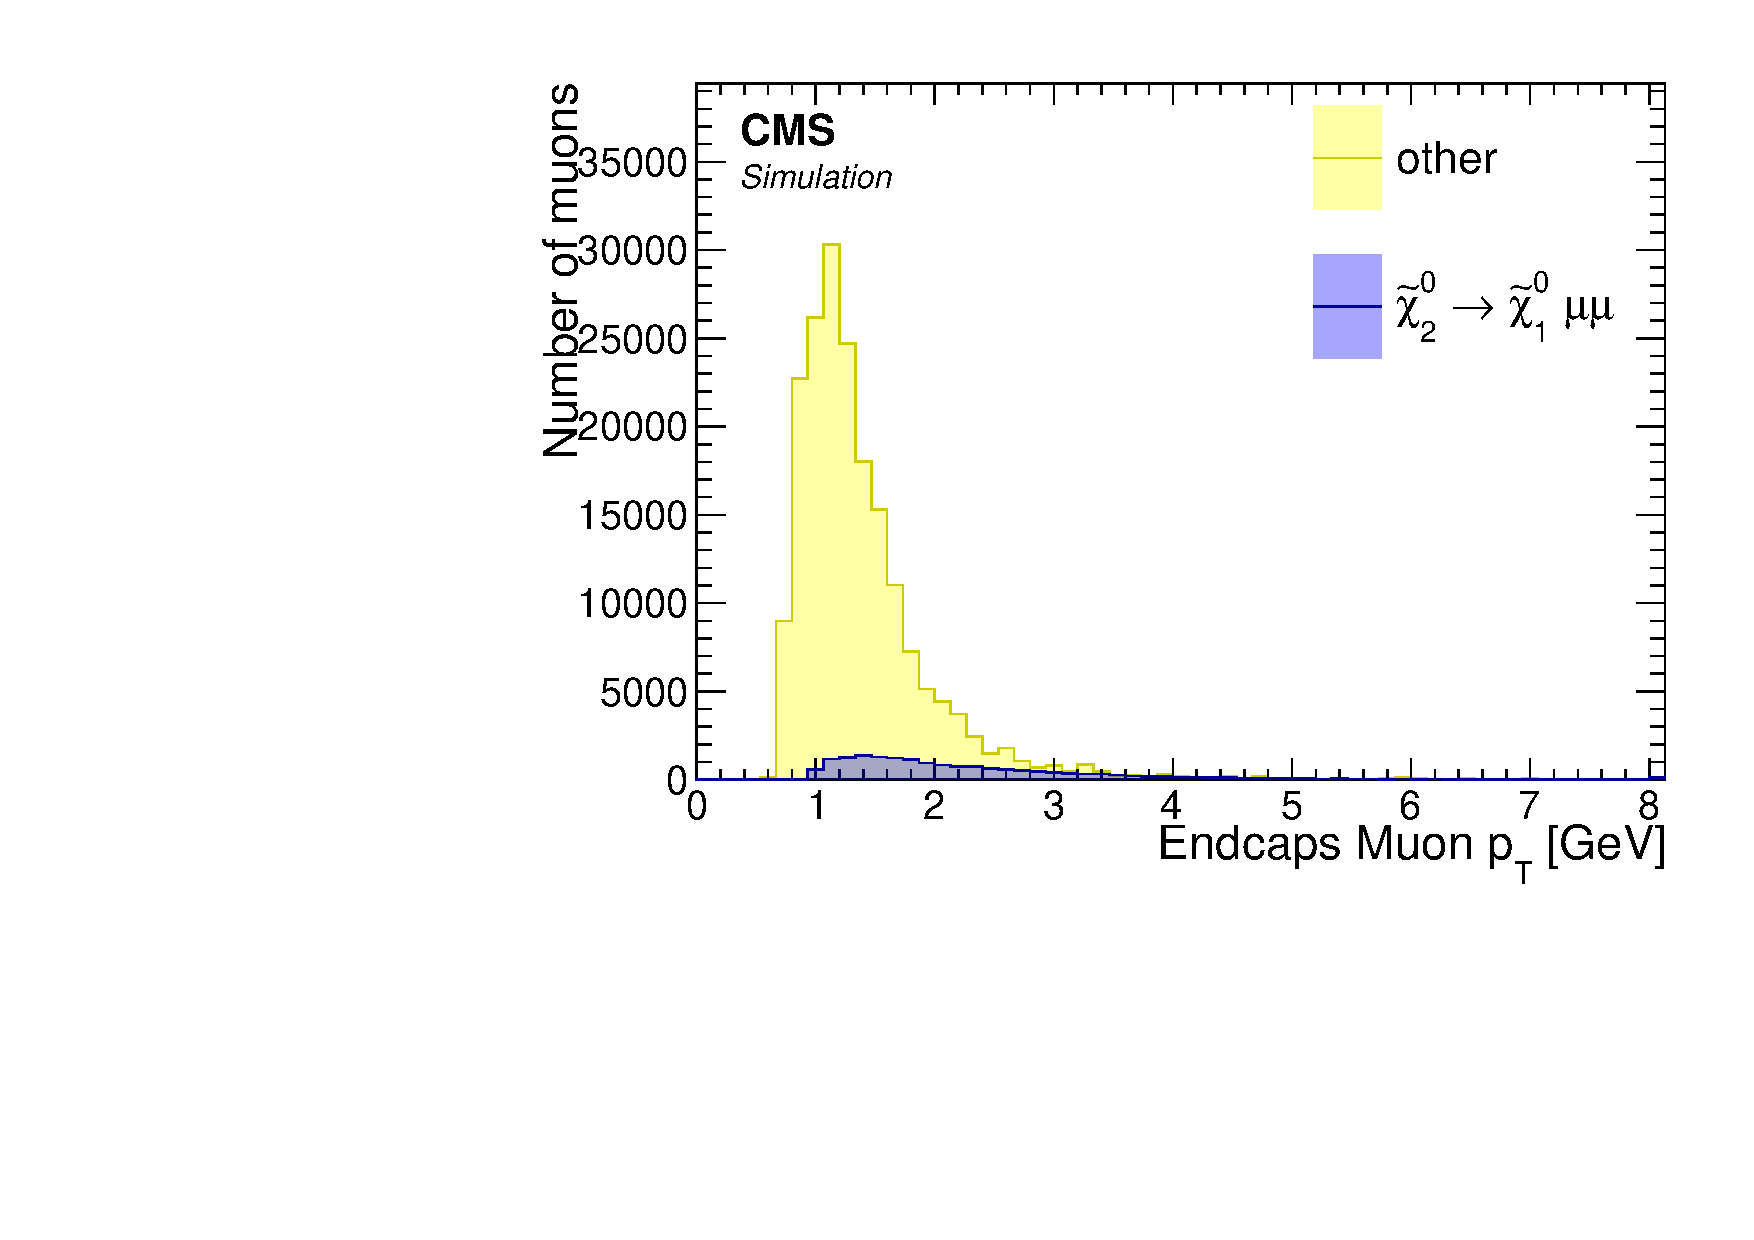
\includegraphics[width=0.32\linewidth]{plots/lepton_selection/lepton_selection_dm1p92/none_Muons_pt_endcape.pdf}  \\
\caption[Reconstructed muons \pt]{Reconstructed muons \pt distibution with loose ID for $\dm=5.63\GeV$ (top) and $\dm=1.92\GeV$ (bottom) in the inclusive case (left), barrel (middle) and endcaps (right). Cuts of $\DR(\jmath_1,\mu)>0.4$ and $\pt<15\GeV$ are applied.}
\label{fig:muons-selectrion-pt}
\end{figure}

We can see the point being made earlier about the endcaps being able to reconstruct muons with lower\pt, and therefore has worse purity than the barrel reiterated here. It must be stressed that worse purity is due to a much higher efficiency, and therefore, as long as we can purify it further, is not necessarily a bad thing. We see however, that the bulk of the non-signal muons populate the region of $\pt<2\GeV$, and the ratio of signal muons to non-signal muons is very low in that region. We therefore make an additional cut of $\pt>2\GeV$. Another way of looking at the effect of this cut is by looking at the $\abs{\eta}$ distribution before and after the \pt cut which can be seen in~\ref{fig:muons-selection-eta}.

\begin{figure}[!htb]
\centering
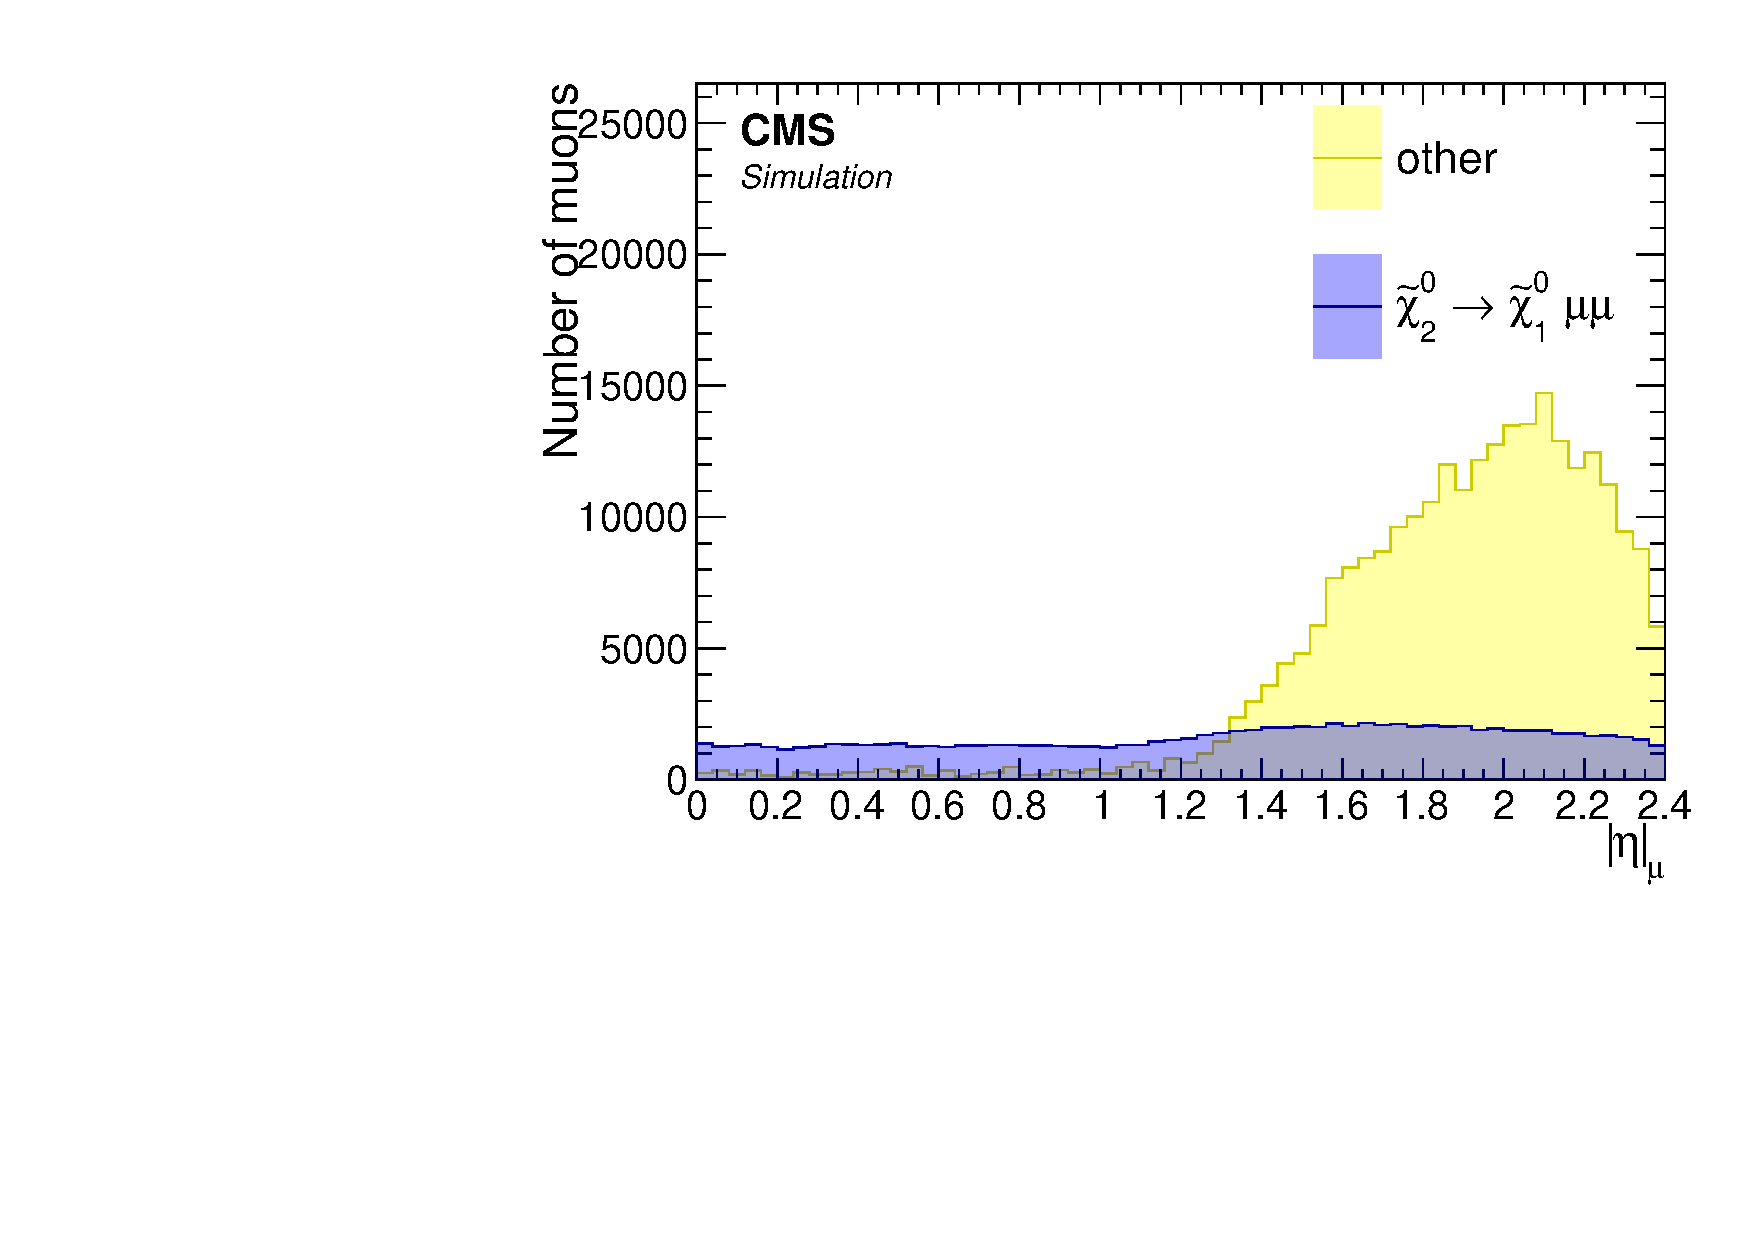
\includegraphics[width=0.48\linewidth]{plots/lepton_selection/lepton_selection_dm5p63/none_Muons_Eta.pdf} \,
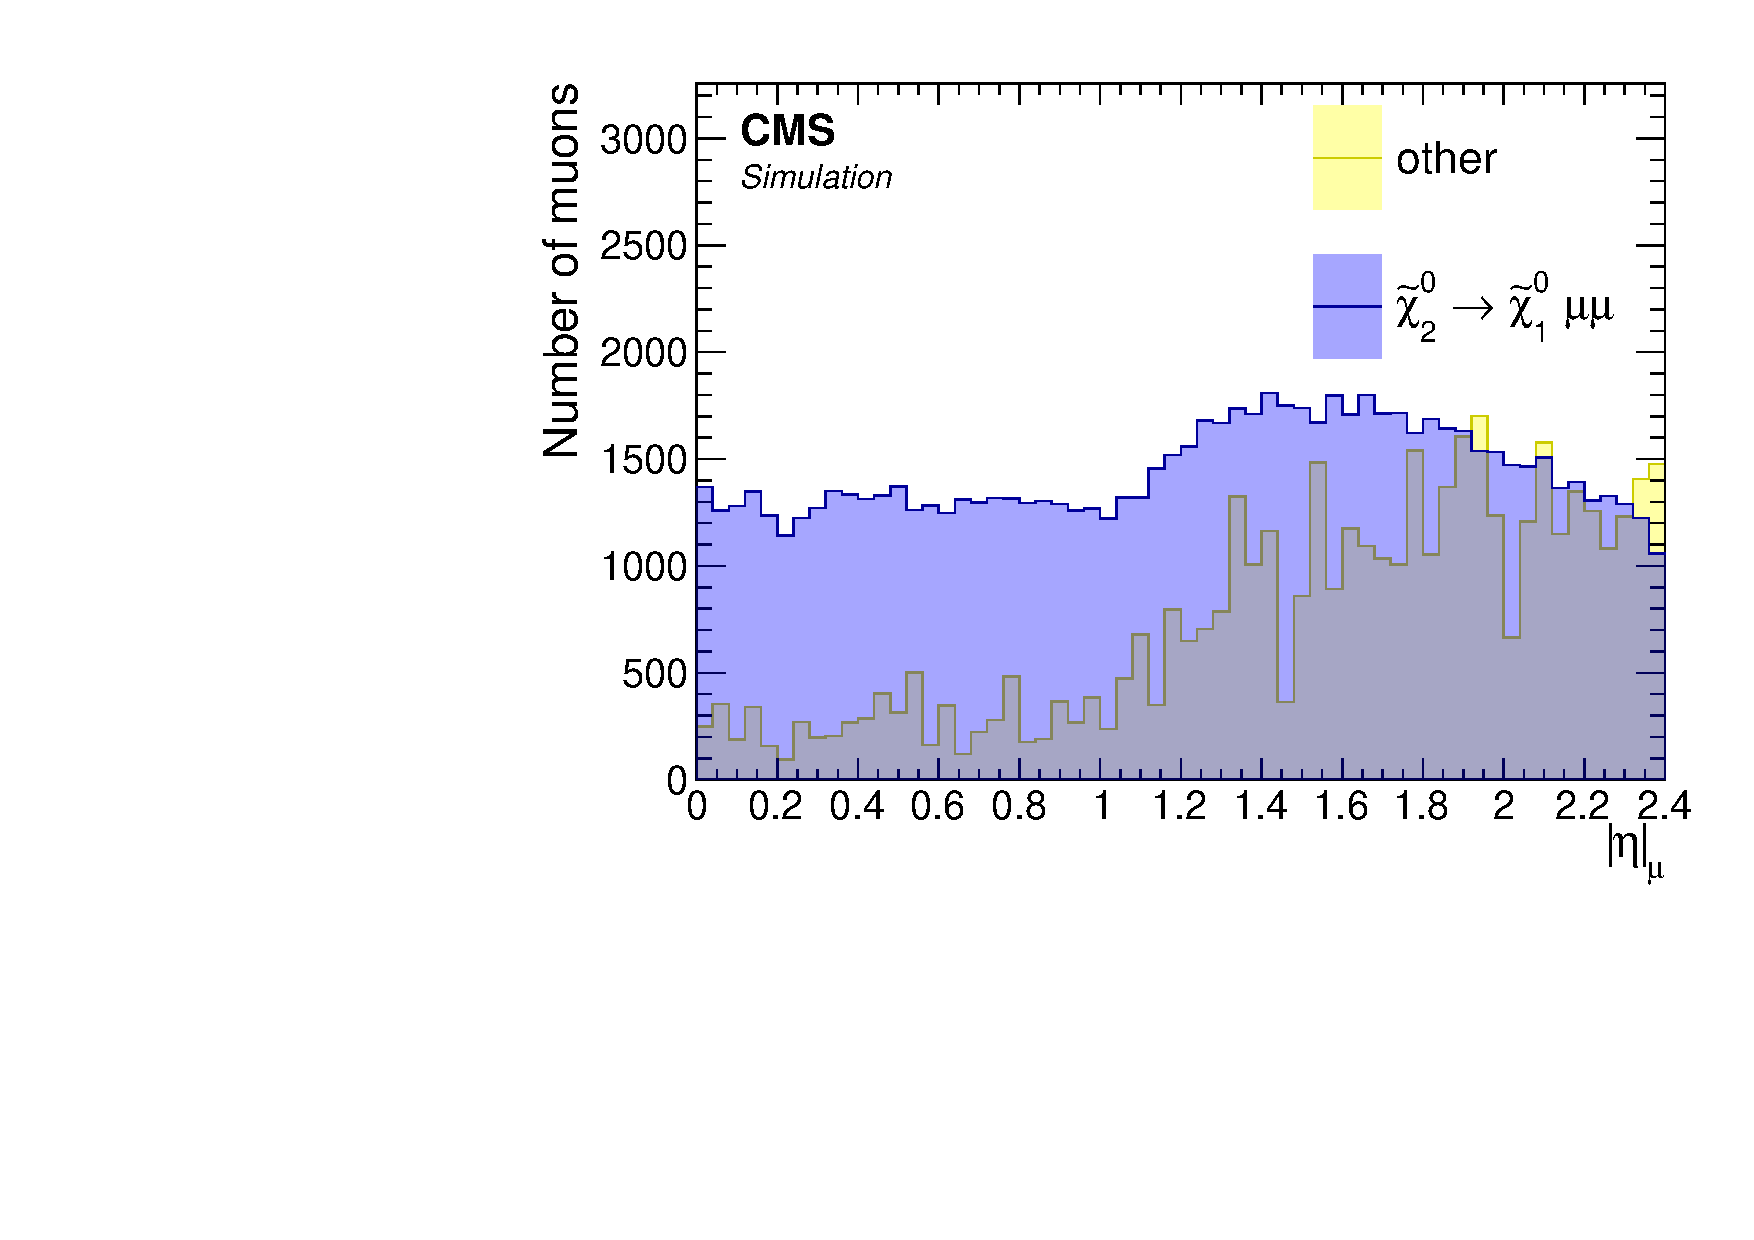
\includegraphics[width=0.48\linewidth]{plots/lepton_selection/lepton_selection_dm5p63/none_Muons_Eta_after_pt.pdf} \\
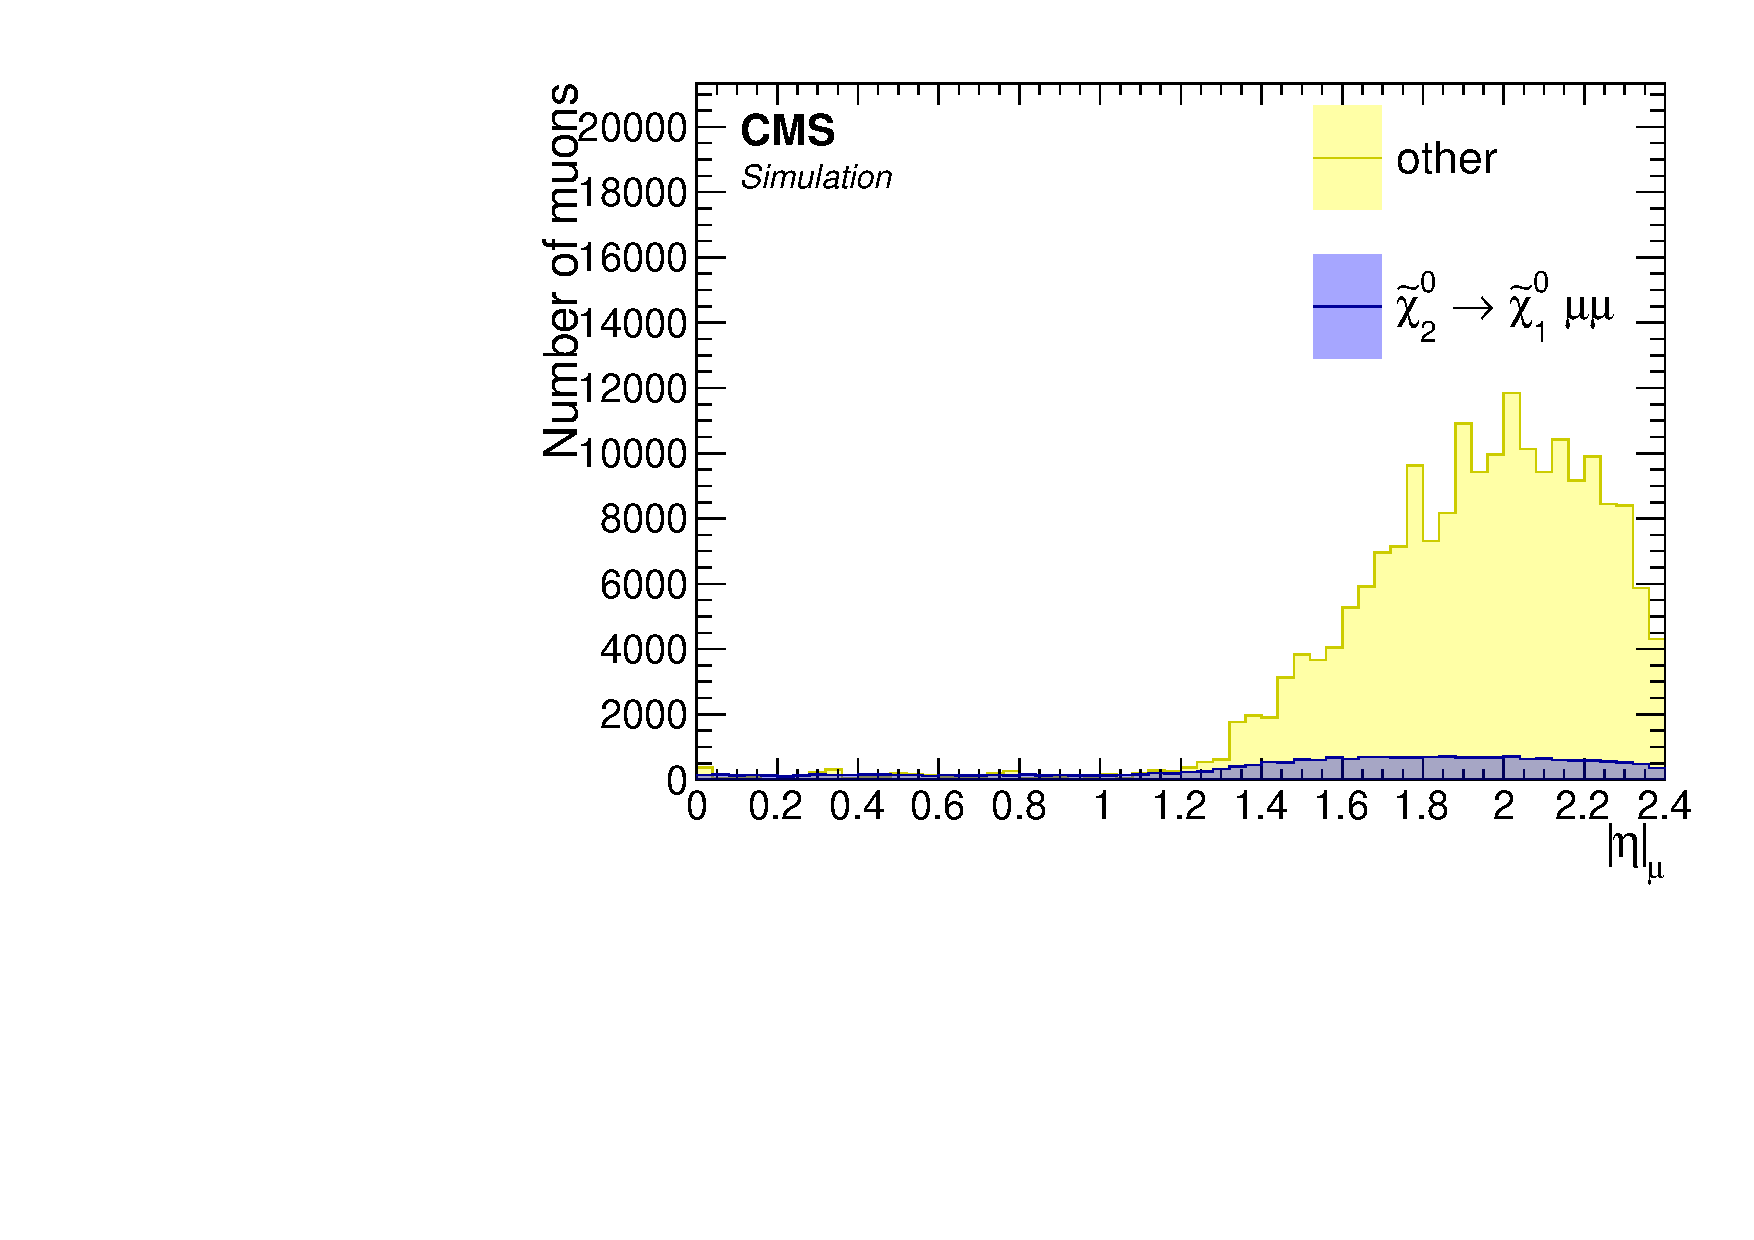
\includegraphics[width=0.48\linewidth]{plots/lepton_selection/lepton_selection_dm1p92/none_Muons_Eta.pdf}  \,
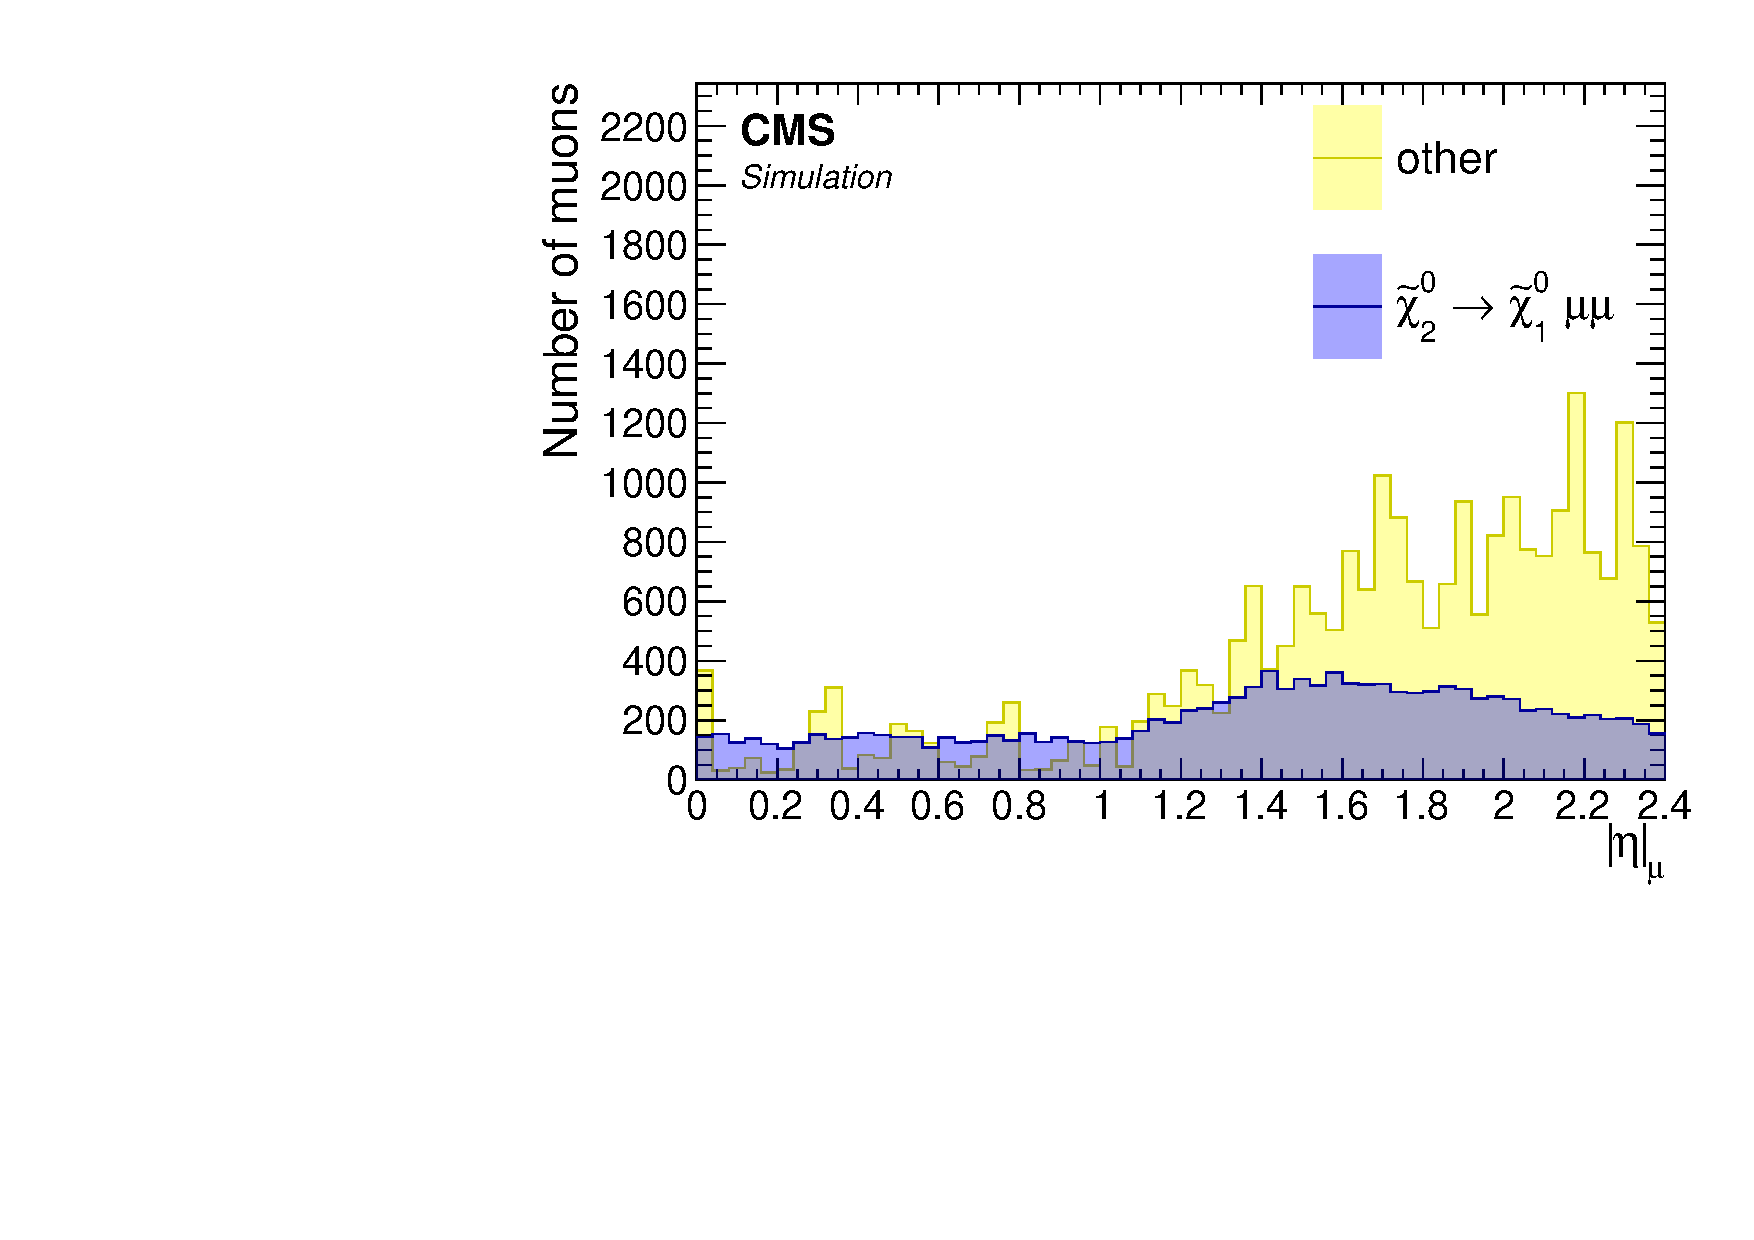
\includegraphics[width=0.48\linewidth]{plots/lepton_selection/lepton_selection_dm1p92/none_Muons_Eta_after_pt.pdf} \\
\caption[\abs{\eta} distribution of reconstructed muons with loose ID before and after $\pt>2\GeV$ cut]{ \abs{\eta} distribution of reconstructed muons with loose ID for $\dm=5.63\GeV$ (top) and $\dm=1.92\GeV$ (bottom) without (left) and with (right) $\pt>2\GeV$ cut. Cut of $\DR(\jmath_1,\mu)>0.4$ is also applied.}
\label{fig:muons-selection-eta}
\end{figure}

We would like to see if requiring a tighter working point for the muon-identification is beneficial. The working point used in the previous distributions is loose. We look turn now to check the effects of requiring either a medium working point, or a tight one. We plot two bins labeled \emph{fail} and \emph{pass}, which correspond to whether the muon passes or failed the identification criteria of a medium or tight working points.

\begin{figure}[!htb]
\centering
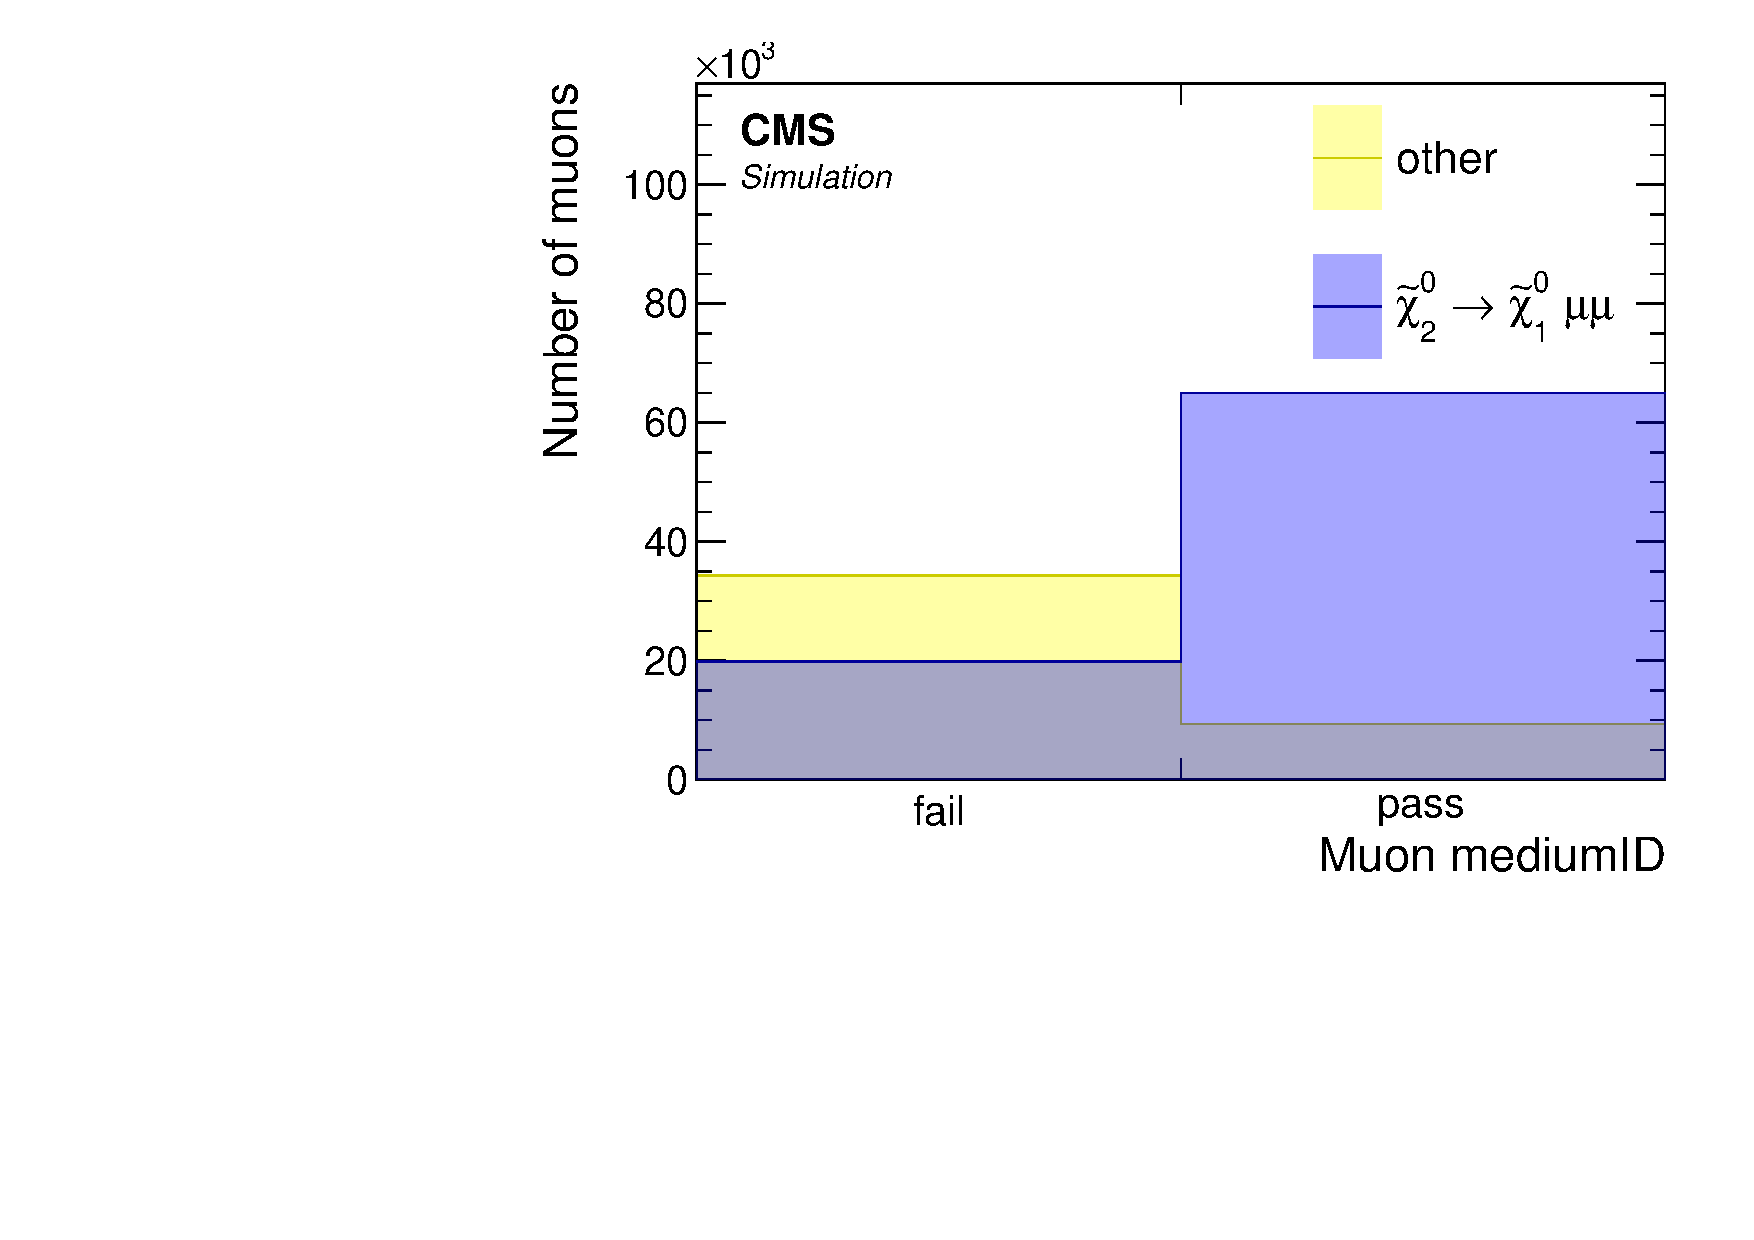
\includegraphics[width=0.32\linewidth]{plots/lepton_selection/lepton_selection_dm5p63/none_Muons_pt_medium.pdf} \,
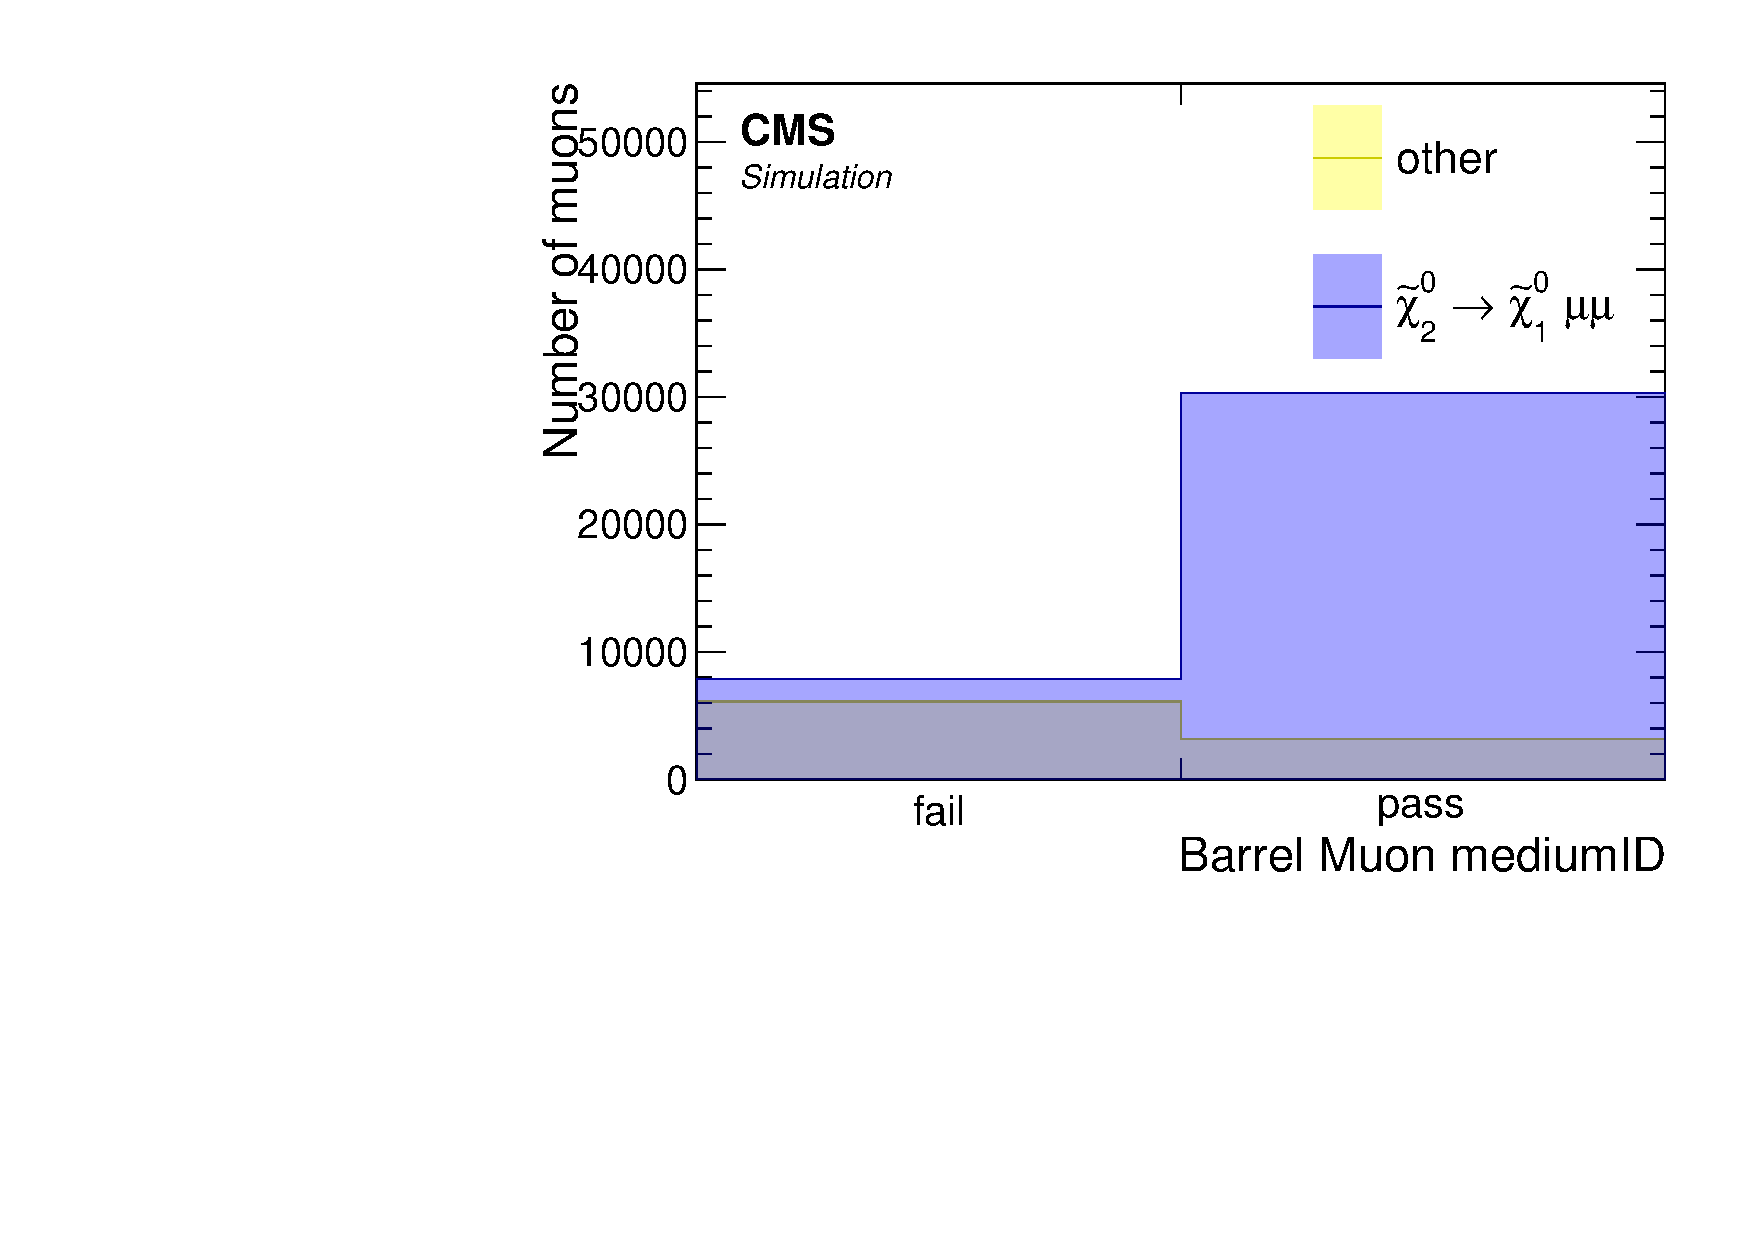
\includegraphics[width=0.32\linewidth]{plots/lepton_selection/lepton_selection_dm5p63/none_Muons_pt_barrel_medium.pdf} \,
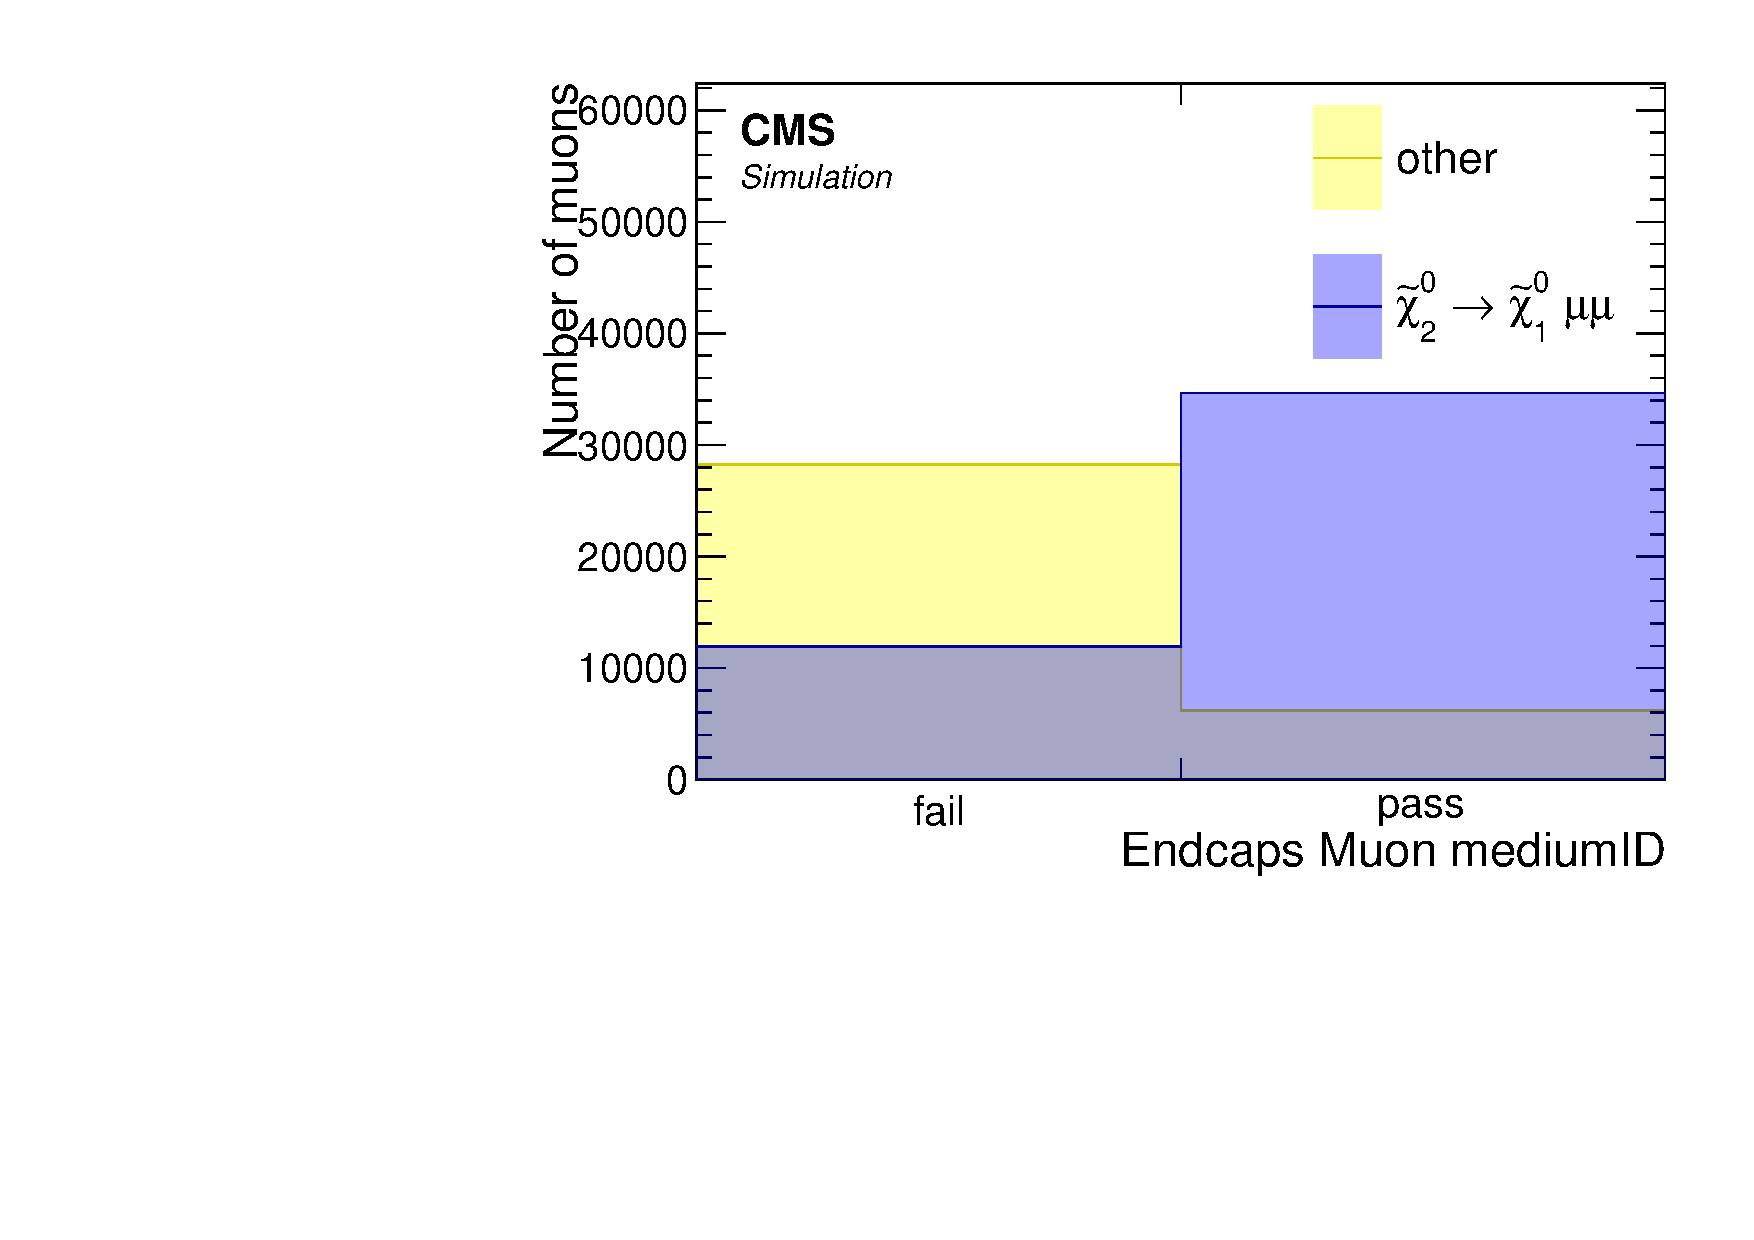
\includegraphics[width=0.32\linewidth]{plots/lepton_selection/lepton_selection_dm5p63/none_Muons_pt_endcape_medium.pdf}   \\
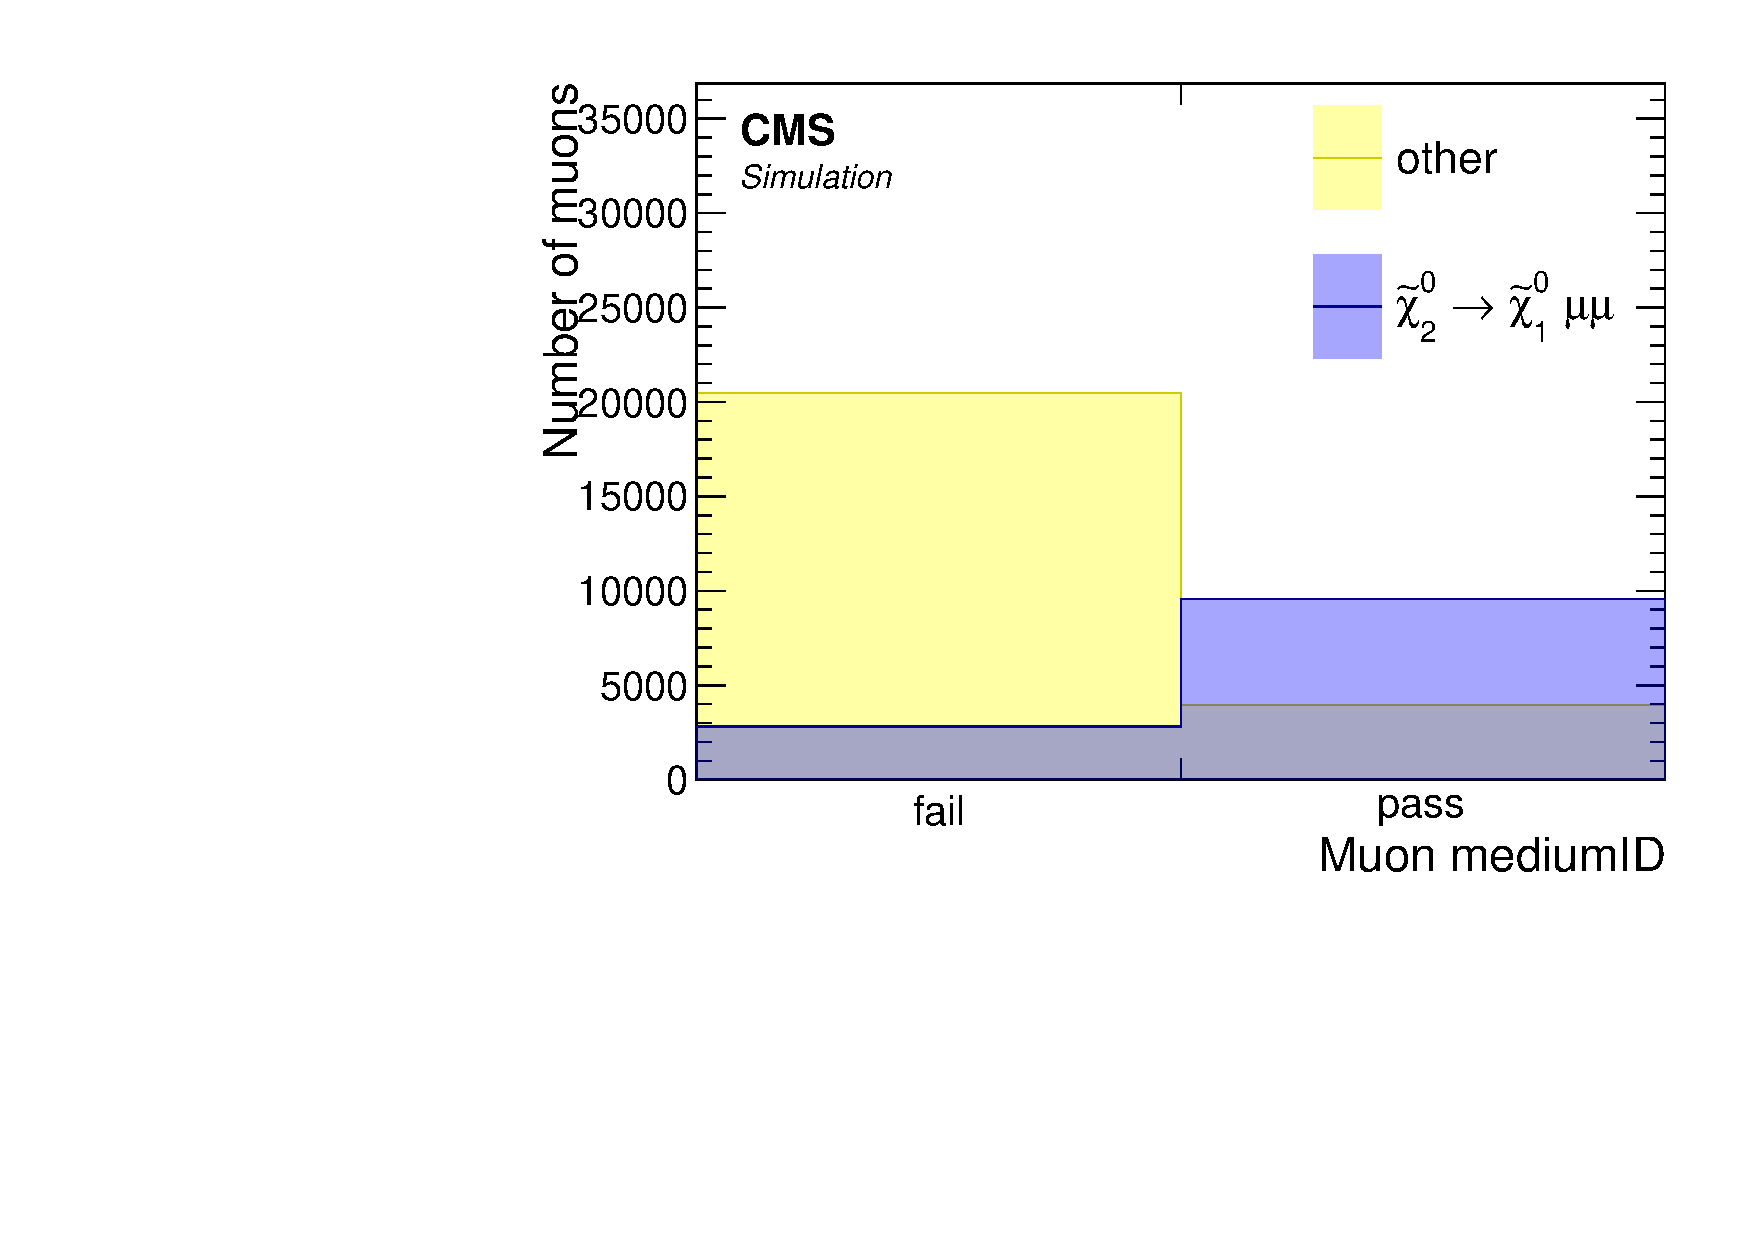
\includegraphics[width=0.32\linewidth]{plots/lepton_selection/lepton_selection_dm1p92/none_Muons_pt_medium.pdf} \,
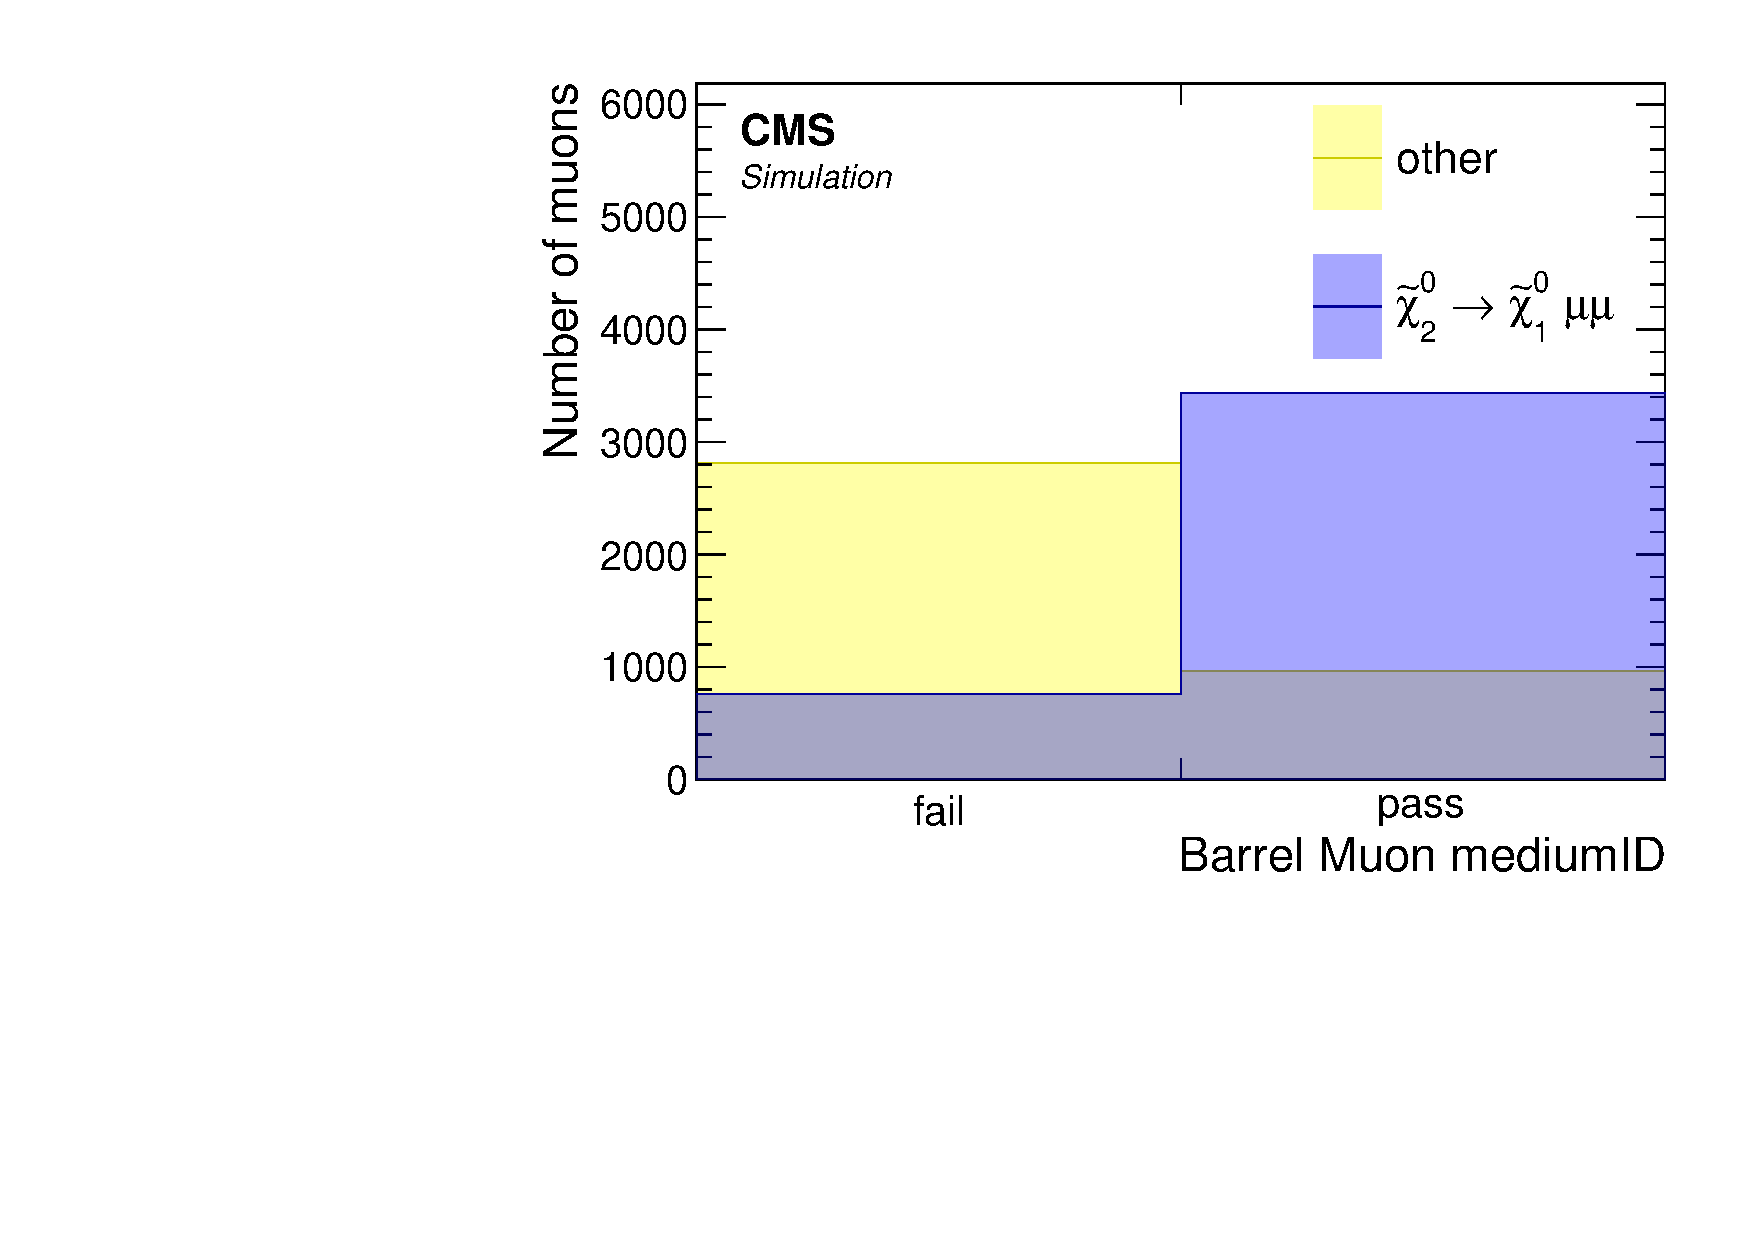
\includegraphics[width=0.32\linewidth]{plots/lepton_selection/lepton_selection_dm1p92/none_Muons_pt_barrel_medium.pdf}  \,
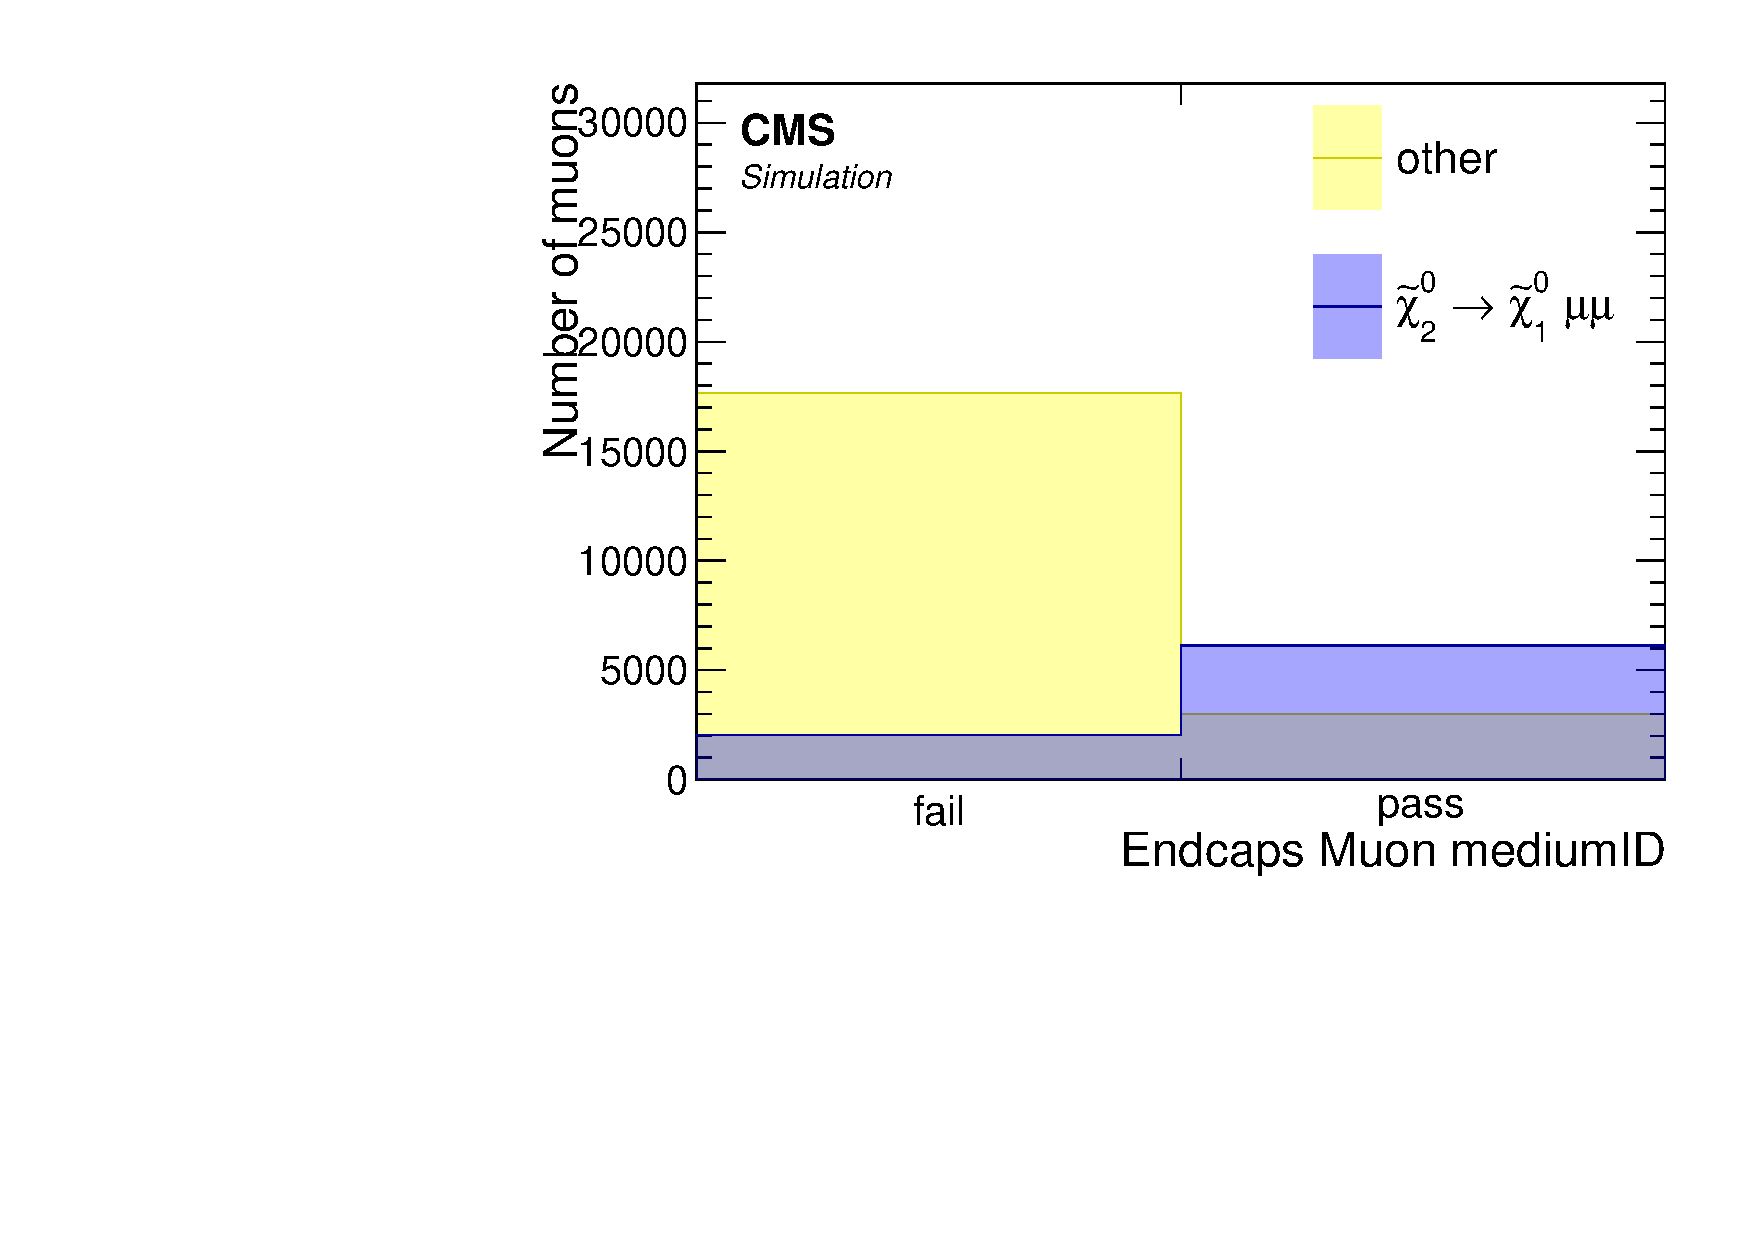
\includegraphics[width=0.32\linewidth]{plots/lepton_selection/lepton_selection_dm1p92/none_Muons_pt_endcape_medium.pdf} \\
\caption[medium ID working point distribution of reconstructed muons]{Medium ID working point distributions of reconstructed muons for $\dm=5.63\GeV$ (top) and $\dm=1.92\GeV$ (bottom) in the inclusive \pt case (left), barrel (middle) and endcaps (right). Cuts of $\DR(\jmath_1,\mu)>0.4$, $\pt>2\GeV$ and $\pt<15\GeV$ are applied.}
\label{fig:muons-selection-id-medium}
\end{figure}

When we compare the medium working point in~\ref{fig:muons-selection-id-medium} to the tight working point in~\ref{fig:muons-selection-id-tight} we can see that the medium working point purifies the muons quite a lot and is very beneficial. However, when we look at the tight working point, we observe that we lose quite a lot of our wanted signal-muons without a significant gain in purity. We therefore choose to use the medium ID working point. 

\begin{figure}[!htb]
\centering
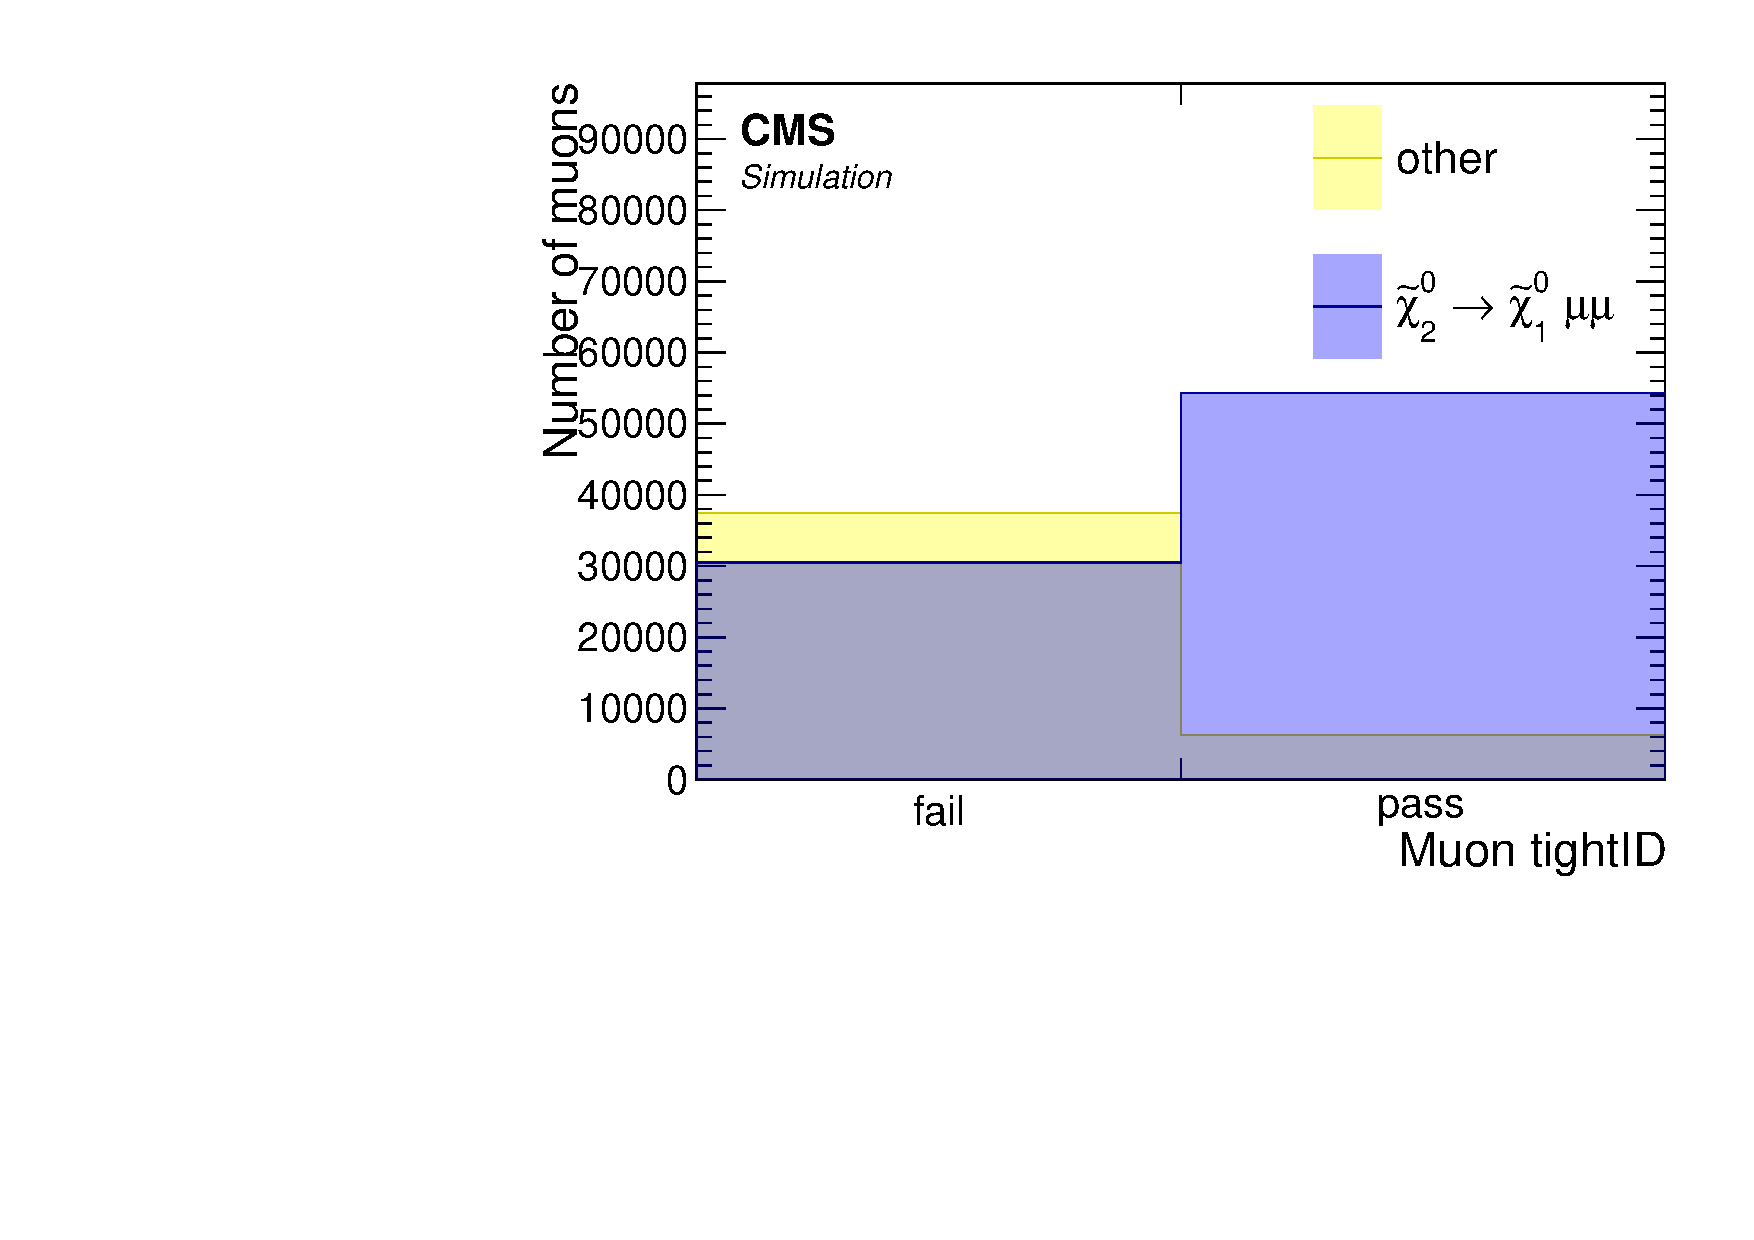
\includegraphics[width=0.32\linewidth]{plots/lepton_selection/lepton_selection_dm5p63/none_Muons_tight.pdf} \,
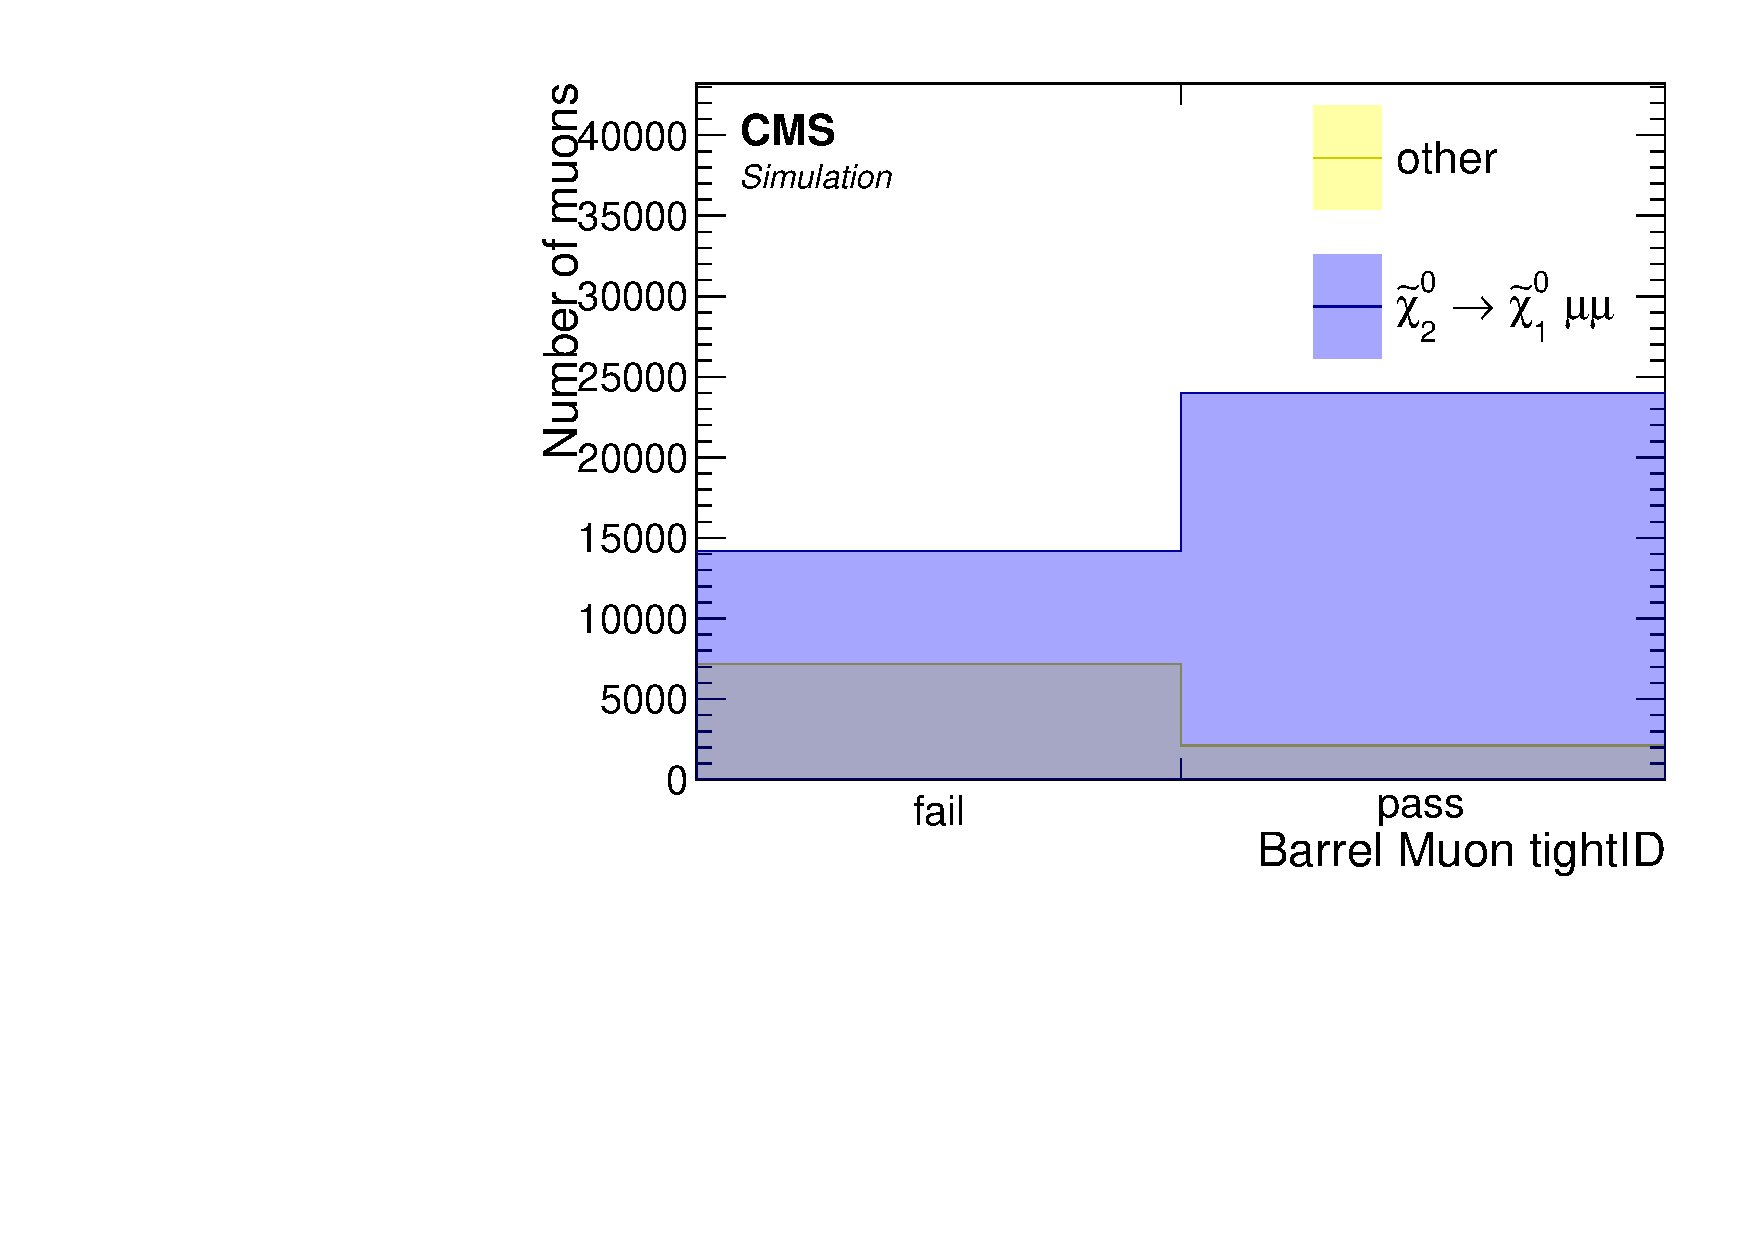
\includegraphics[width=0.32\linewidth]{plots/lepton_selection/lepton_selection_dm5p63/none_Muons_barrel_tight.pdf} \,
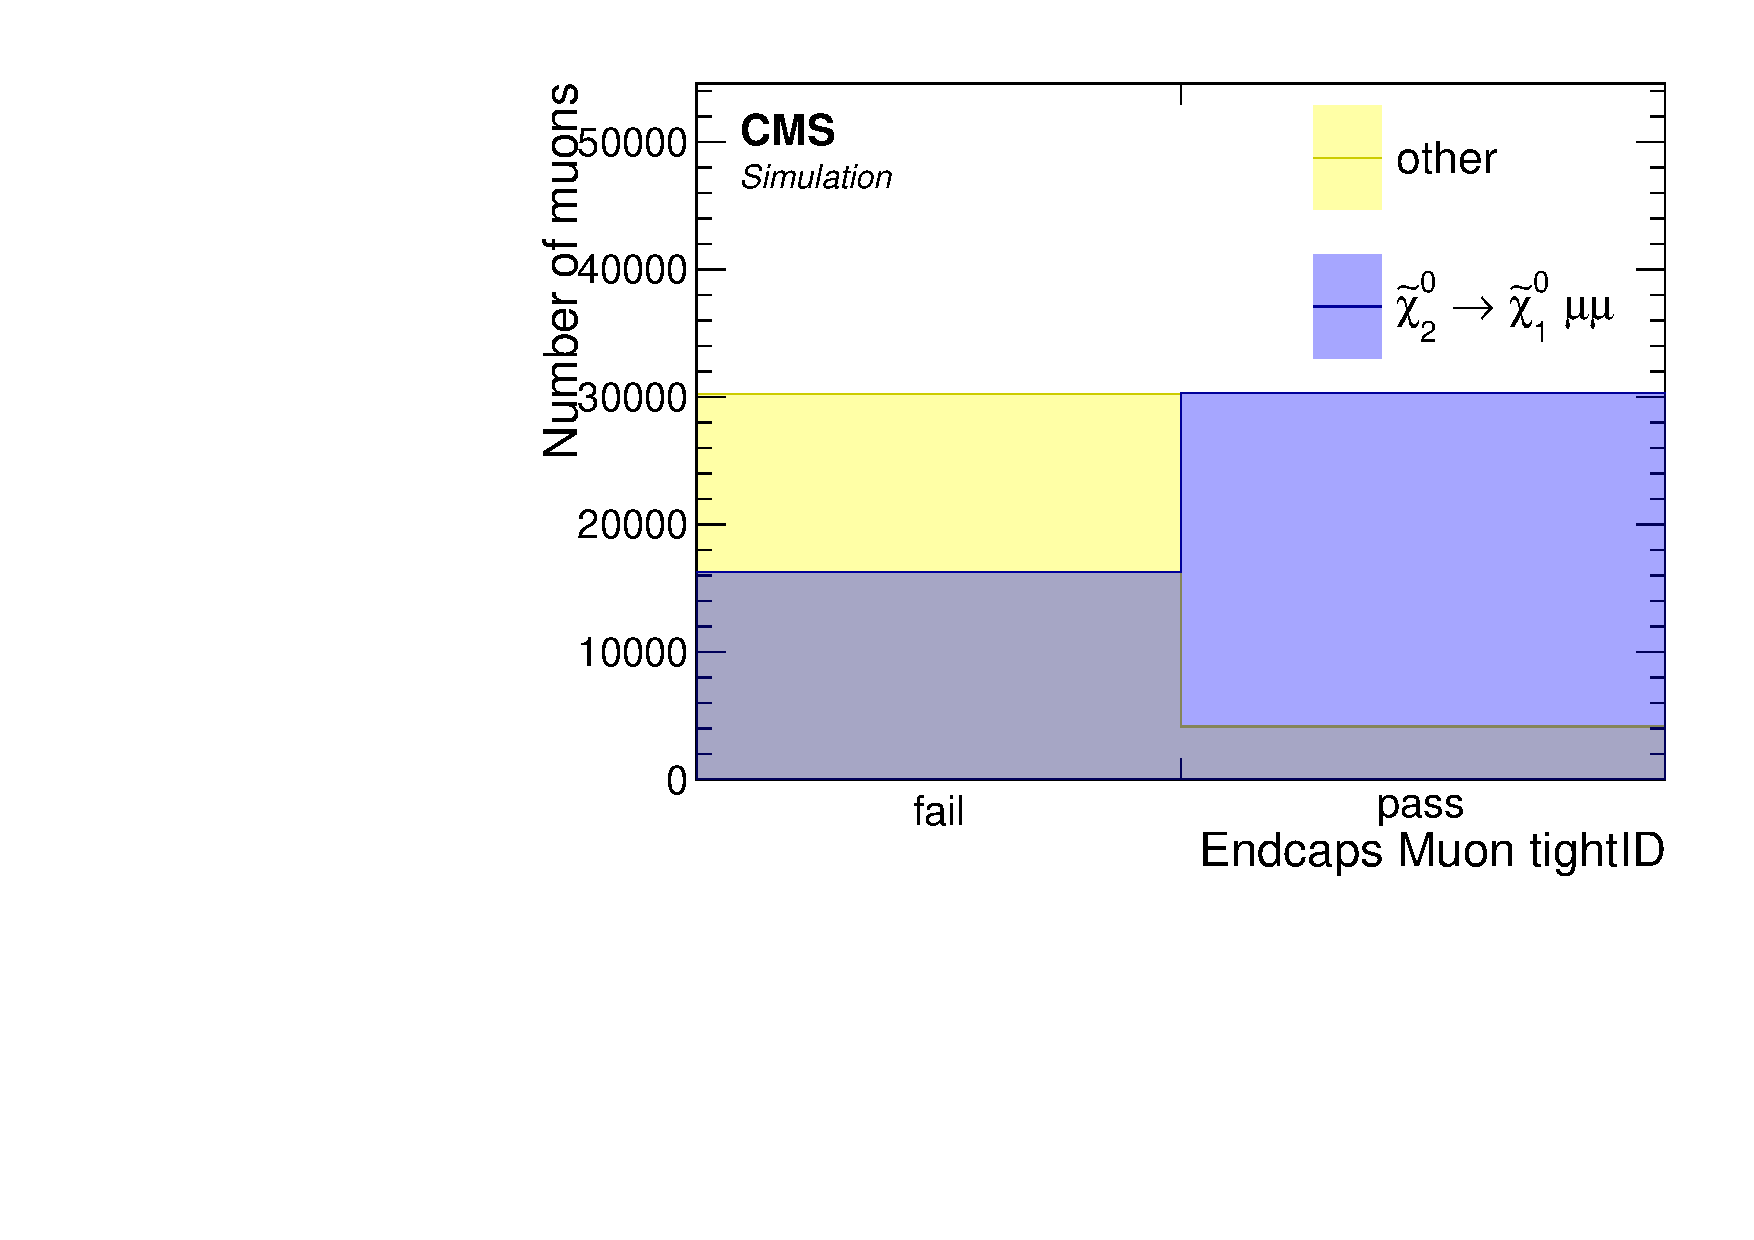
\includegraphics[width=0.32\linewidth]{plots/lepton_selection/lepton_selection_dm5p63/none_Muons_endcape_tight.pdf}   \\
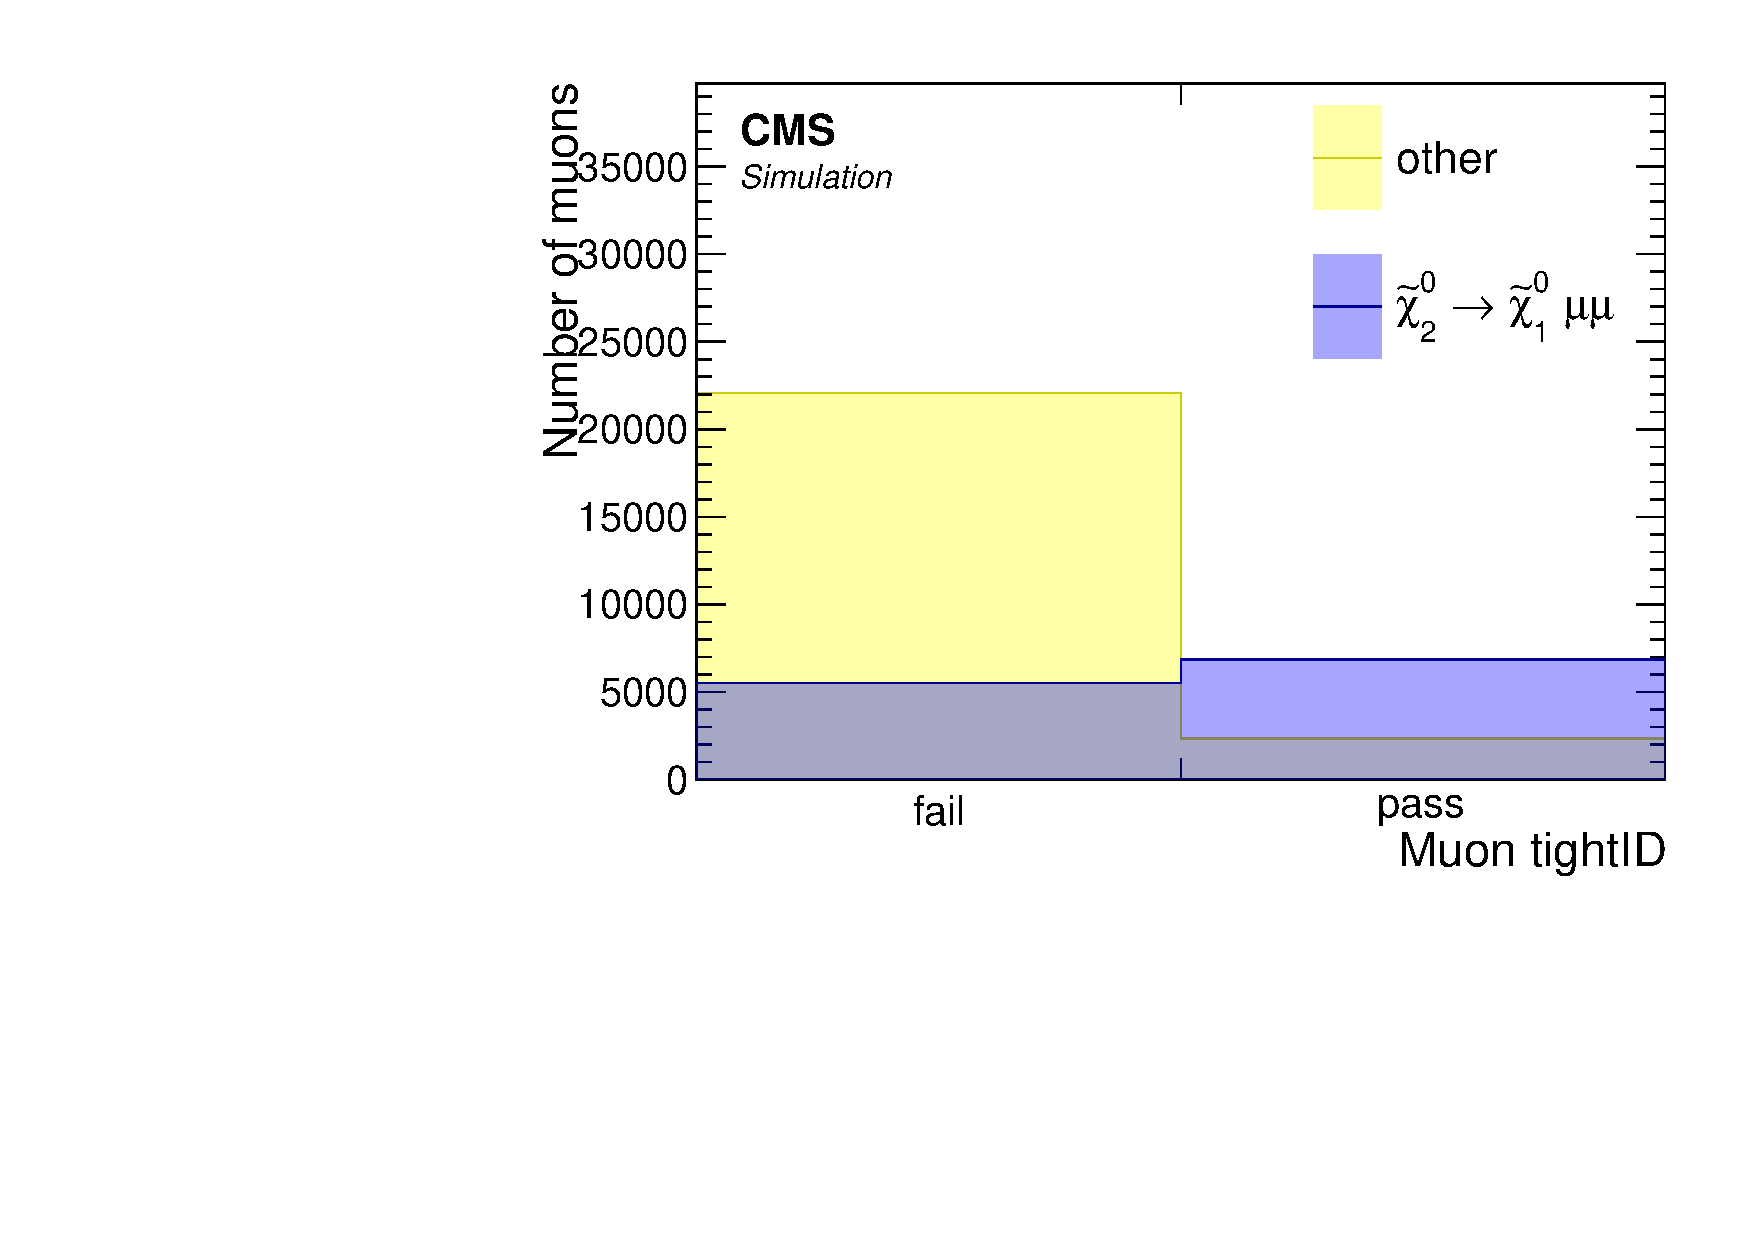
\includegraphics[width=0.32\linewidth]{plots/lepton_selection/lepton_selection_dm1p92/none_Muons_tight.pdf} \,
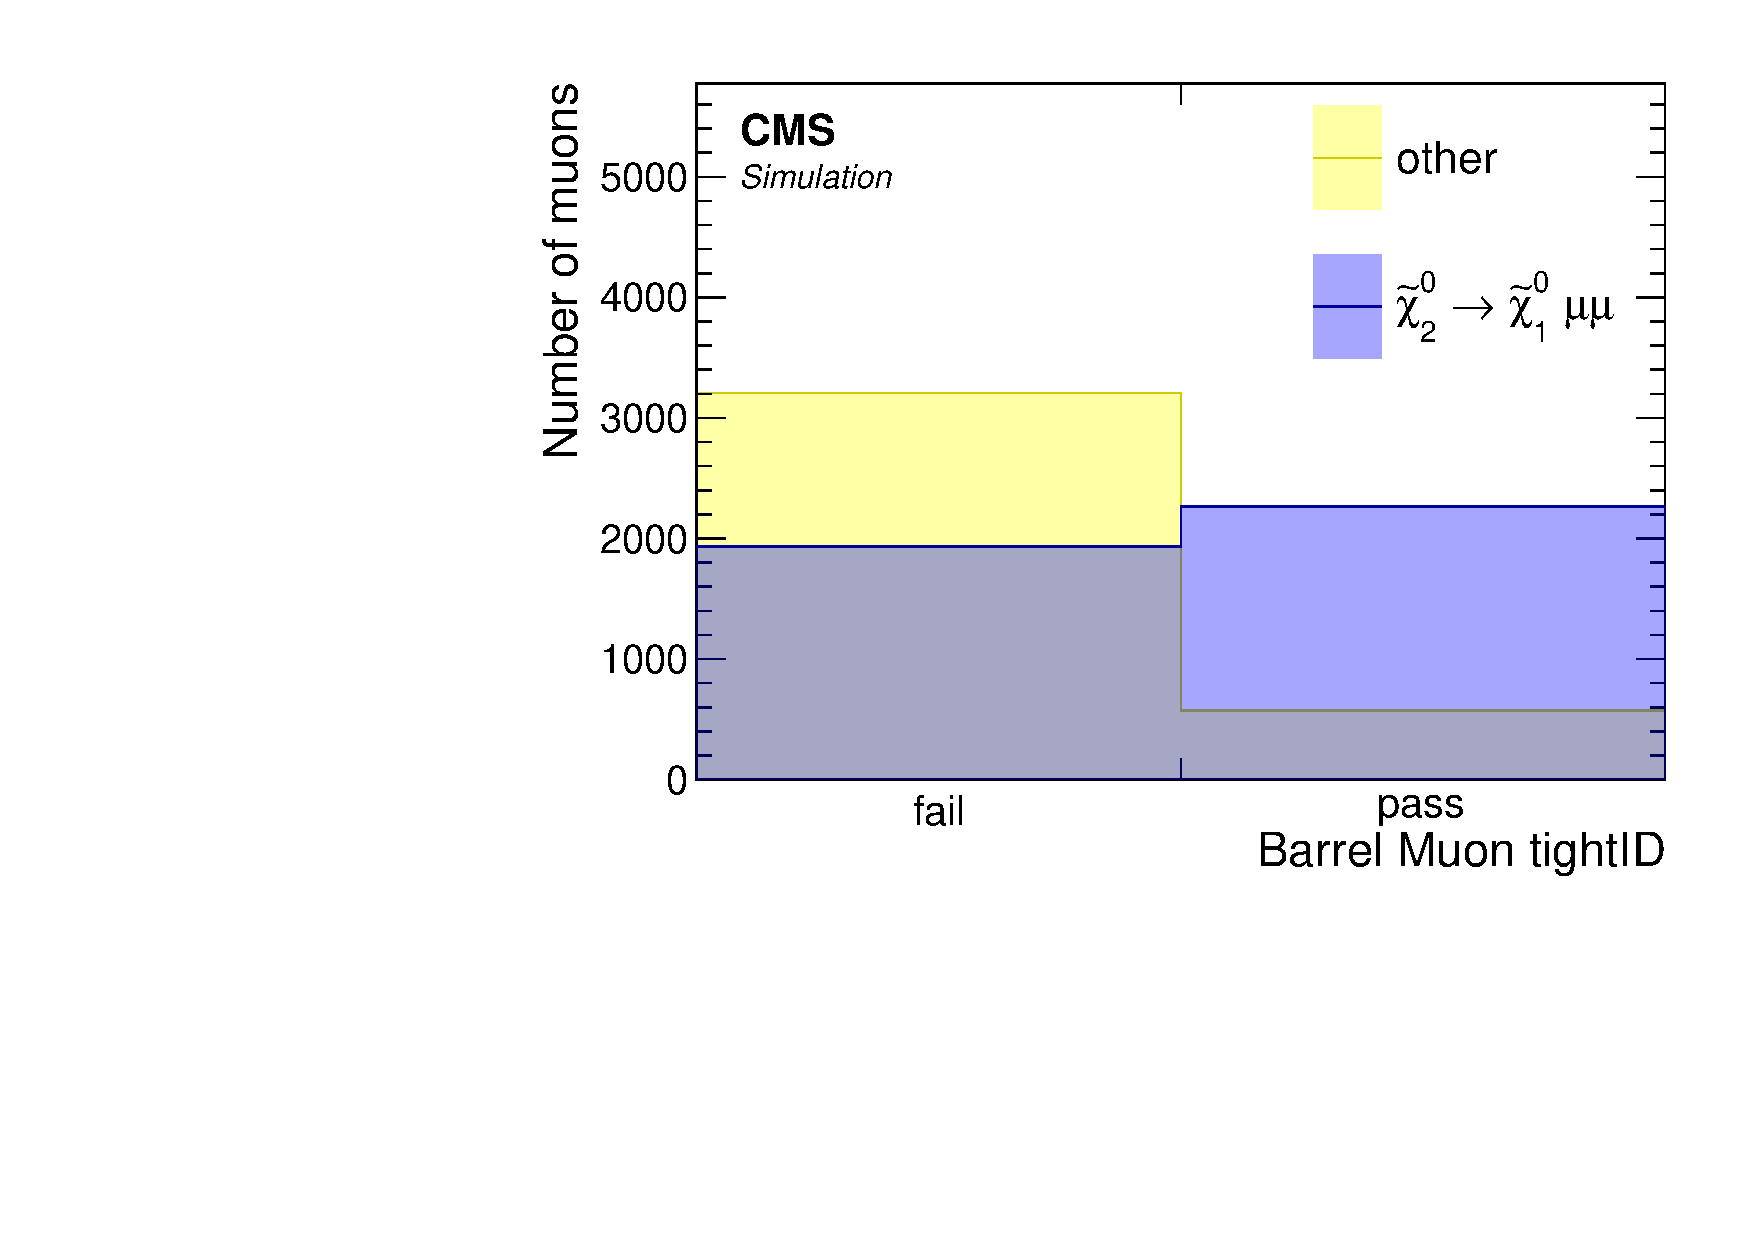
\includegraphics[width=0.32\linewidth]{plots/lepton_selection/lepton_selection_dm1p92/none_Muons_barrel_tight.pdf}  \,
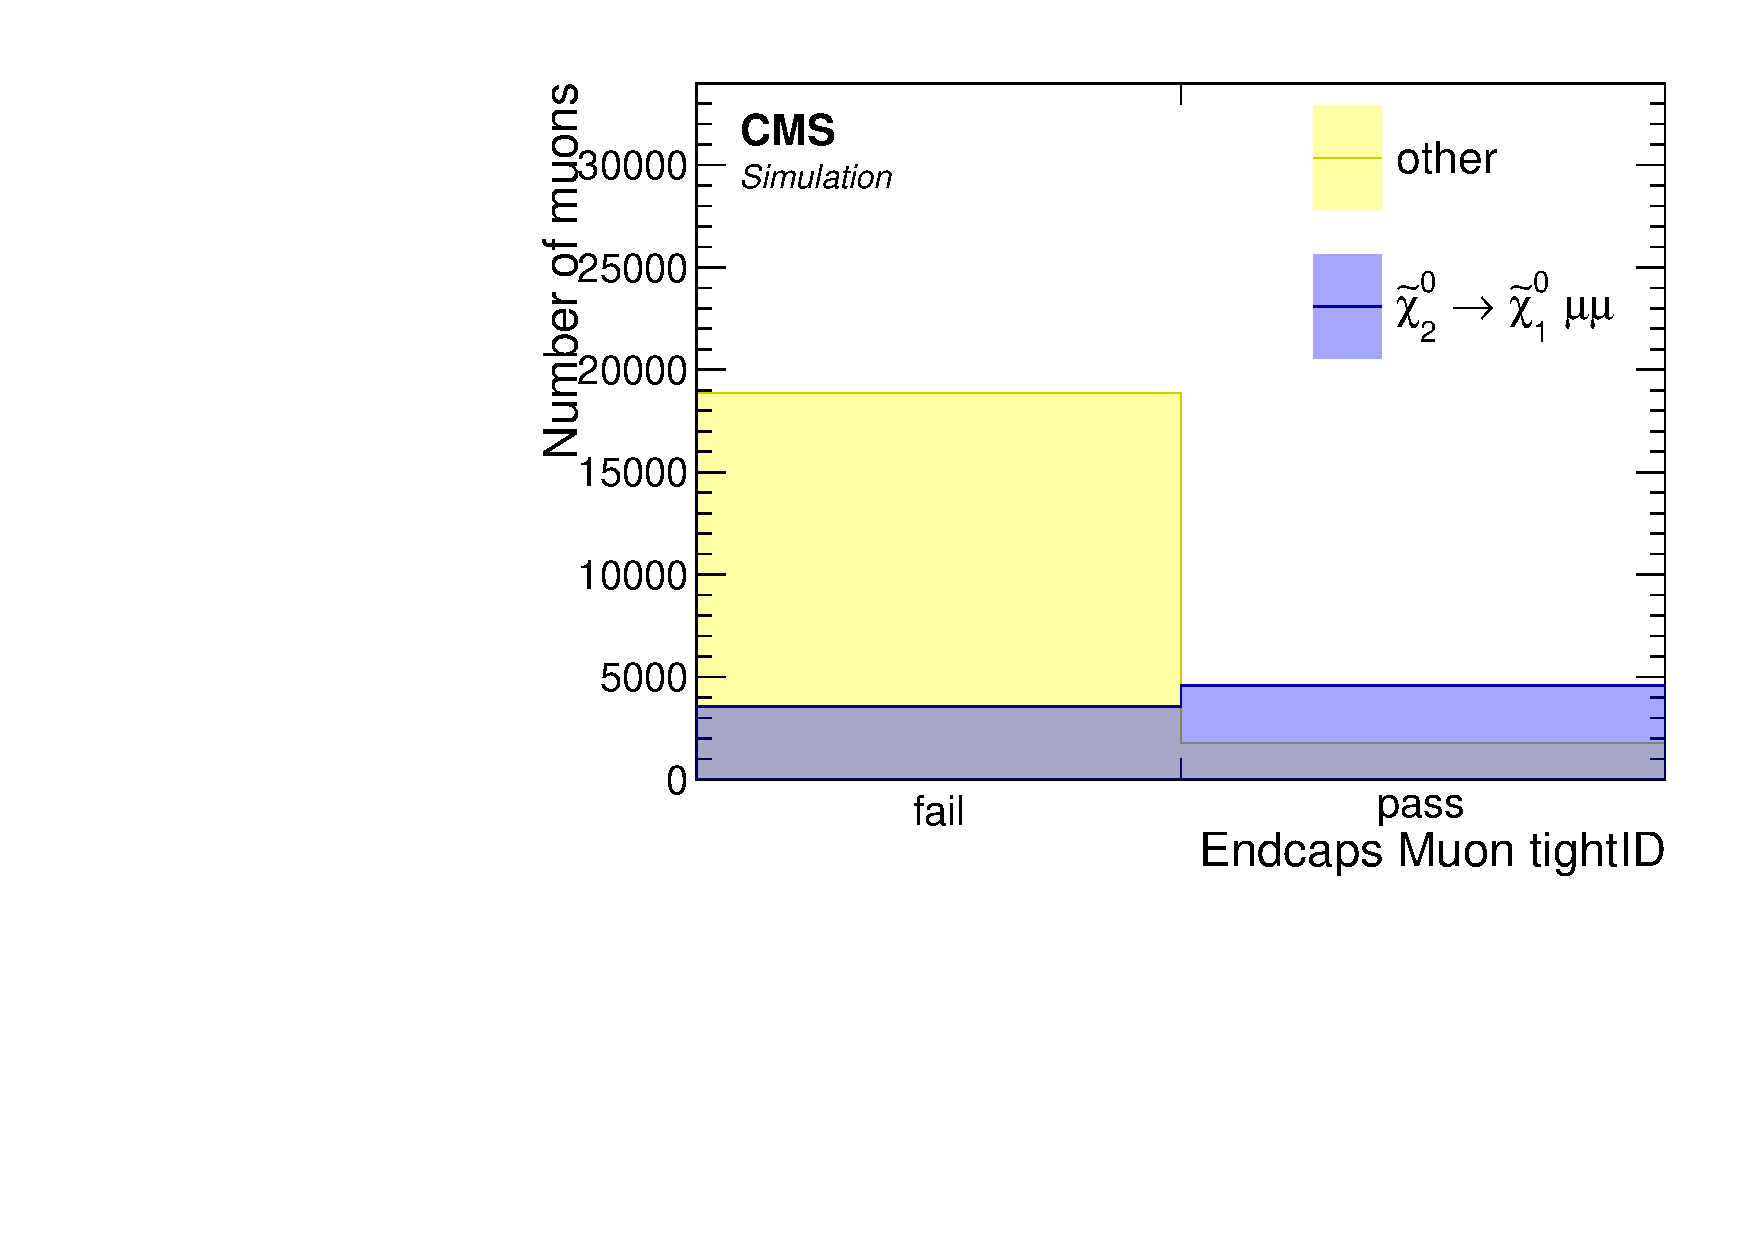
\includegraphics[width=0.32\linewidth]{plots/lepton_selection/lepton_selection_dm1p92/none_Muons_endcape_tight.pdf} \\
\caption[tight ID working point distribution of reconstructed muons]{Tight ID working point distributions of reconstructed muons for $\dm=5.63\GeV$ (top) and $\dm=1.92\GeV$ (bottom) in the inclusive \pt case (left), barrel (middle) and endcaps (right). Cuts of $\DR(\jmath_1,\mu)>0.4$, $\pt>2\GeV$ and $\pt<15\GeV$ are applied.}
\label{fig:muons-selection-id-tight}
\end{figure}

Our custom jet-isolation, which is described fully in~\ref{sec:isolation}, was devised mainly to reject \gls{sm} background while retaining signal. In the electron case, we have seen in ~ref{fig:electrons-selection-isolation} that it did a great job in also purifying the electron selection and replaced the need of requiring a tighter identification working point. In the case of the muons, we do rely on the a medium working point to perform this task, but we would like to also see the effects of the isolation on our signal muons. We see in~\ref{fig:muons-selection-isolation} that we pay a small price by requiring the isolation, but we increase the sensitivity by rejecting a lot of \gls{sm} background in the process.

\begin{figure}[!htb]
\centering
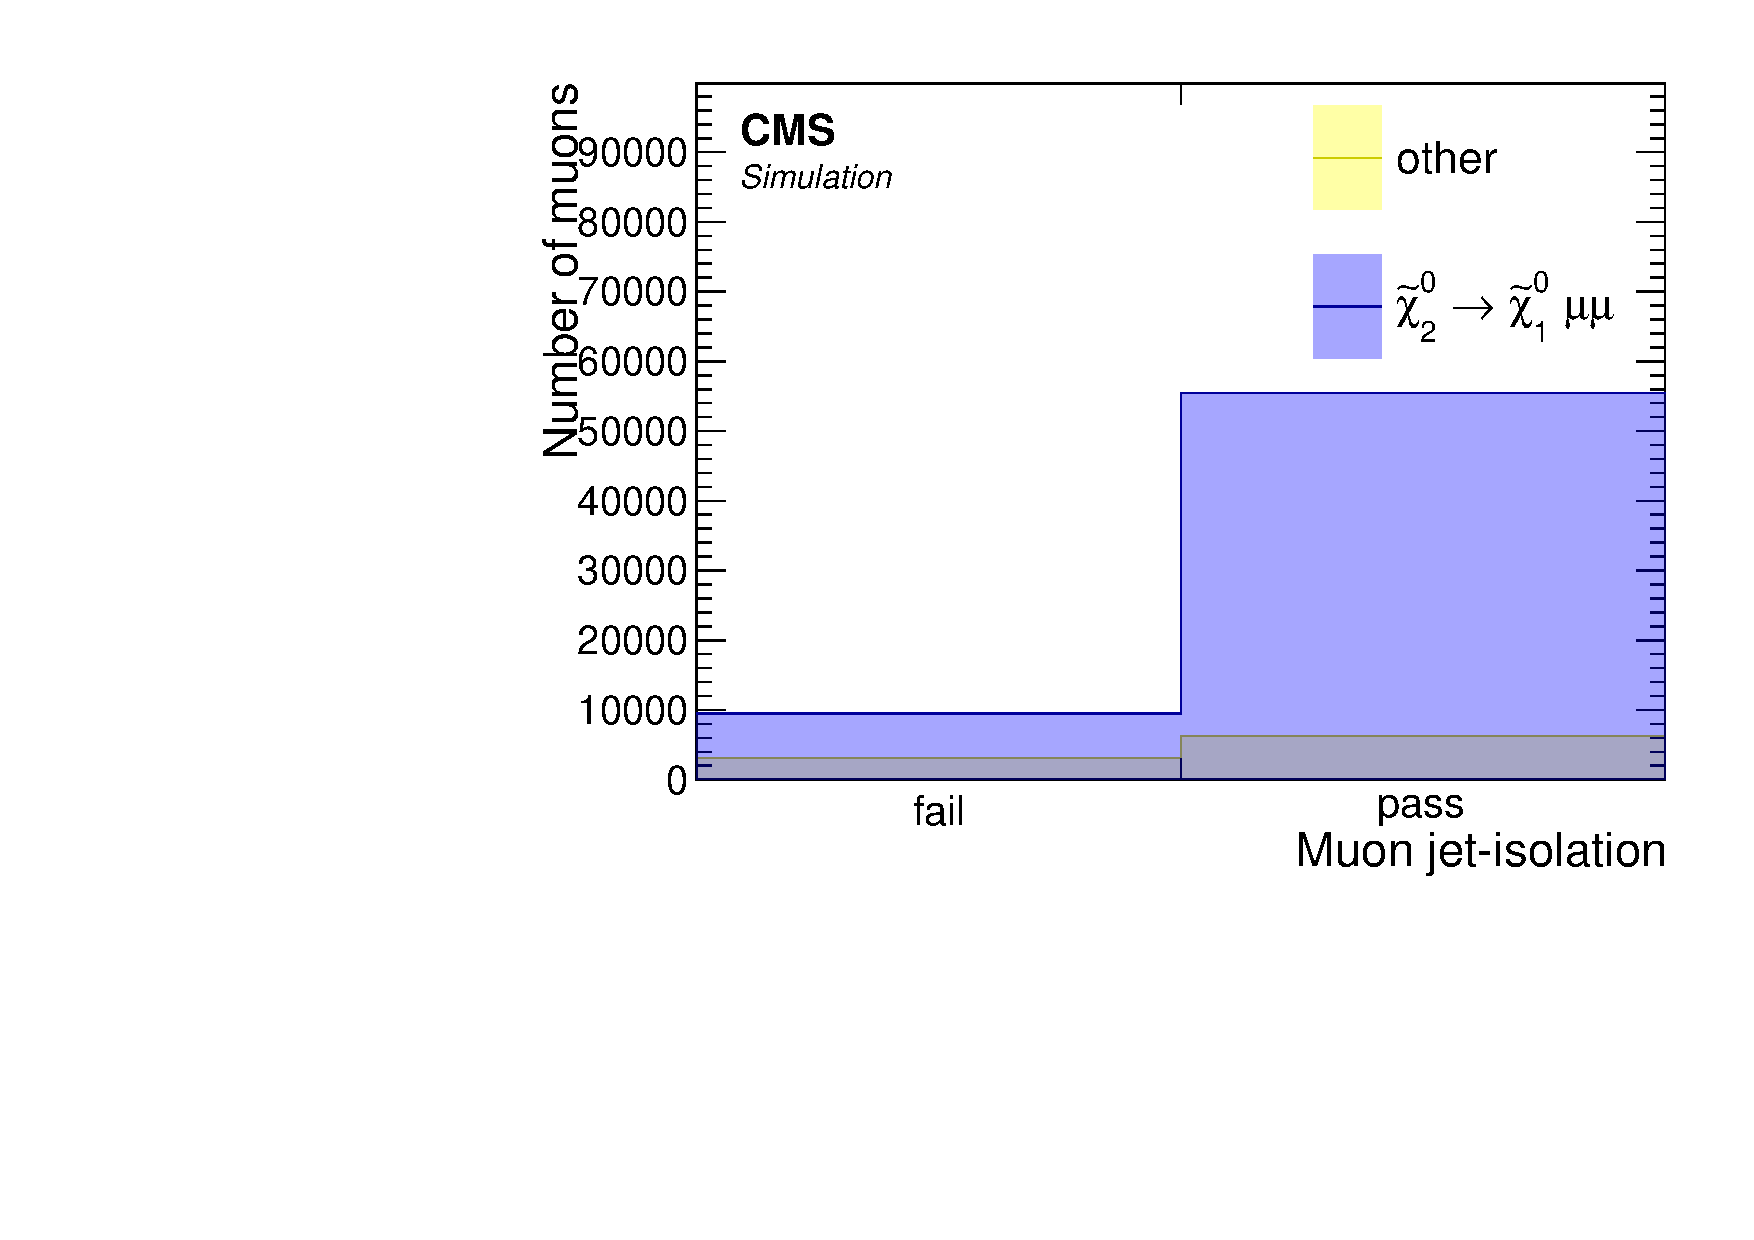
\includegraphics[width=0.32\linewidth]{plots/lepton_selection/lepton_selection_dm5p63/none_Muons_pt_jet_iso.pdf} \,
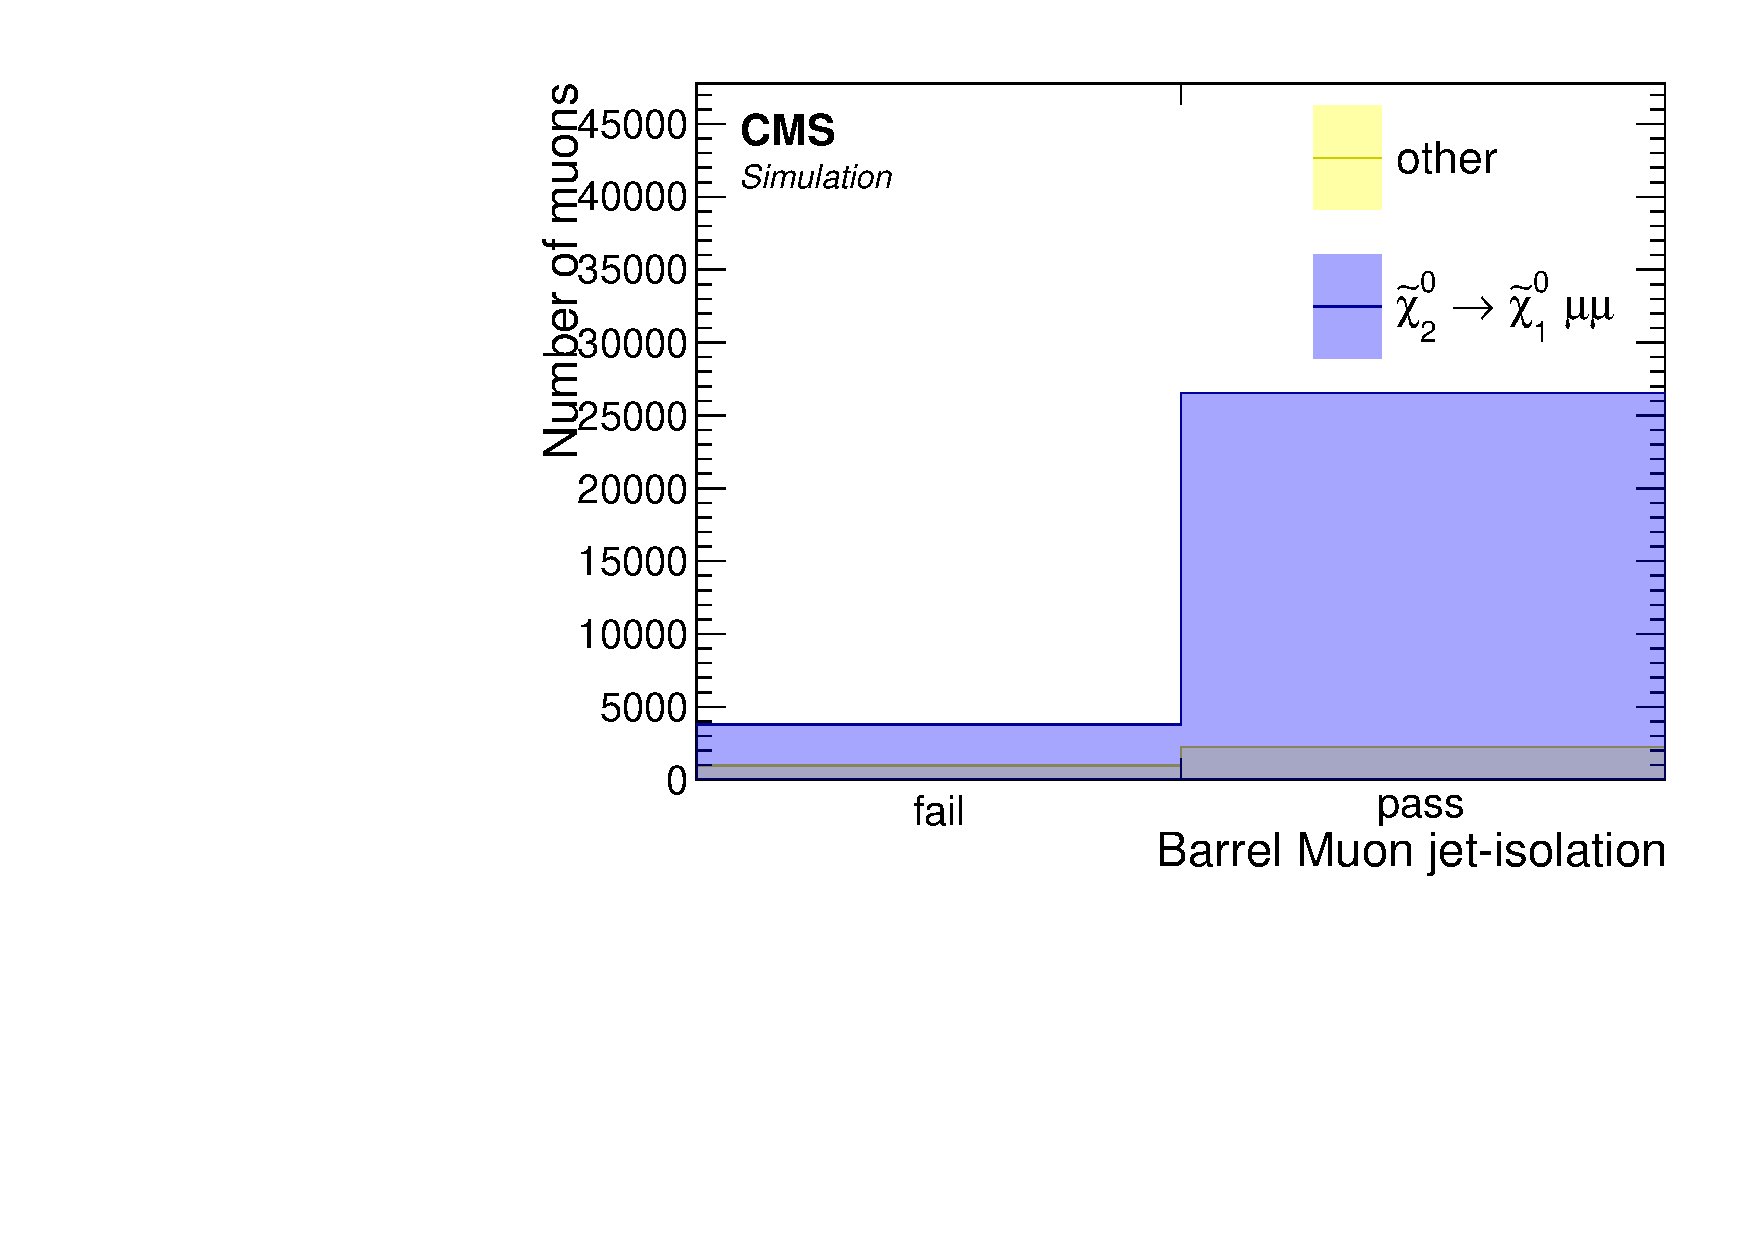
\includegraphics[width=0.32\linewidth]{plots/lepton_selection/lepton_selection_dm5p63/none_Muons_pt_barrel_jet_iso.pdf} \,
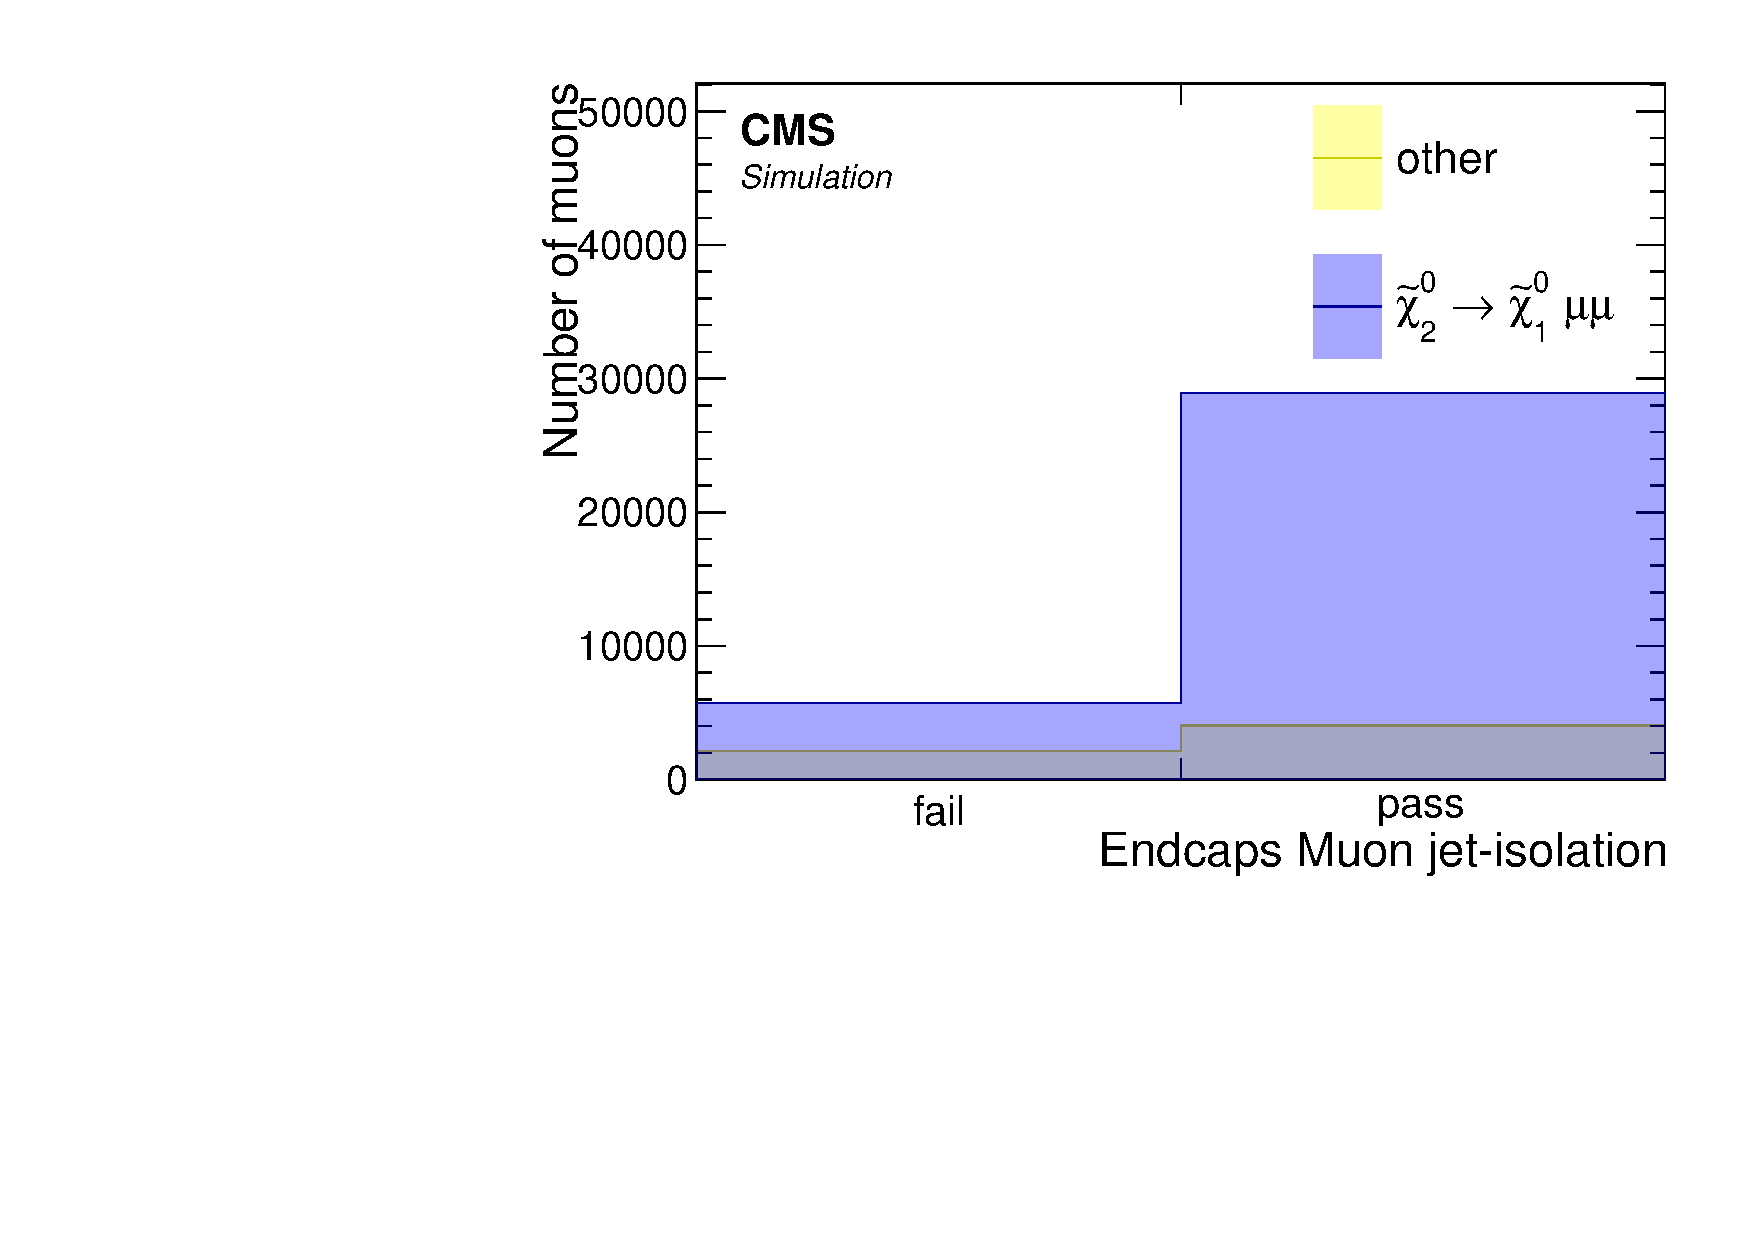
\includegraphics[width=0.32\linewidth]{plots/lepton_selection/lepton_selection_dm5p63/none_Muons_pt_endcape_jet_iso.pdf}   \\
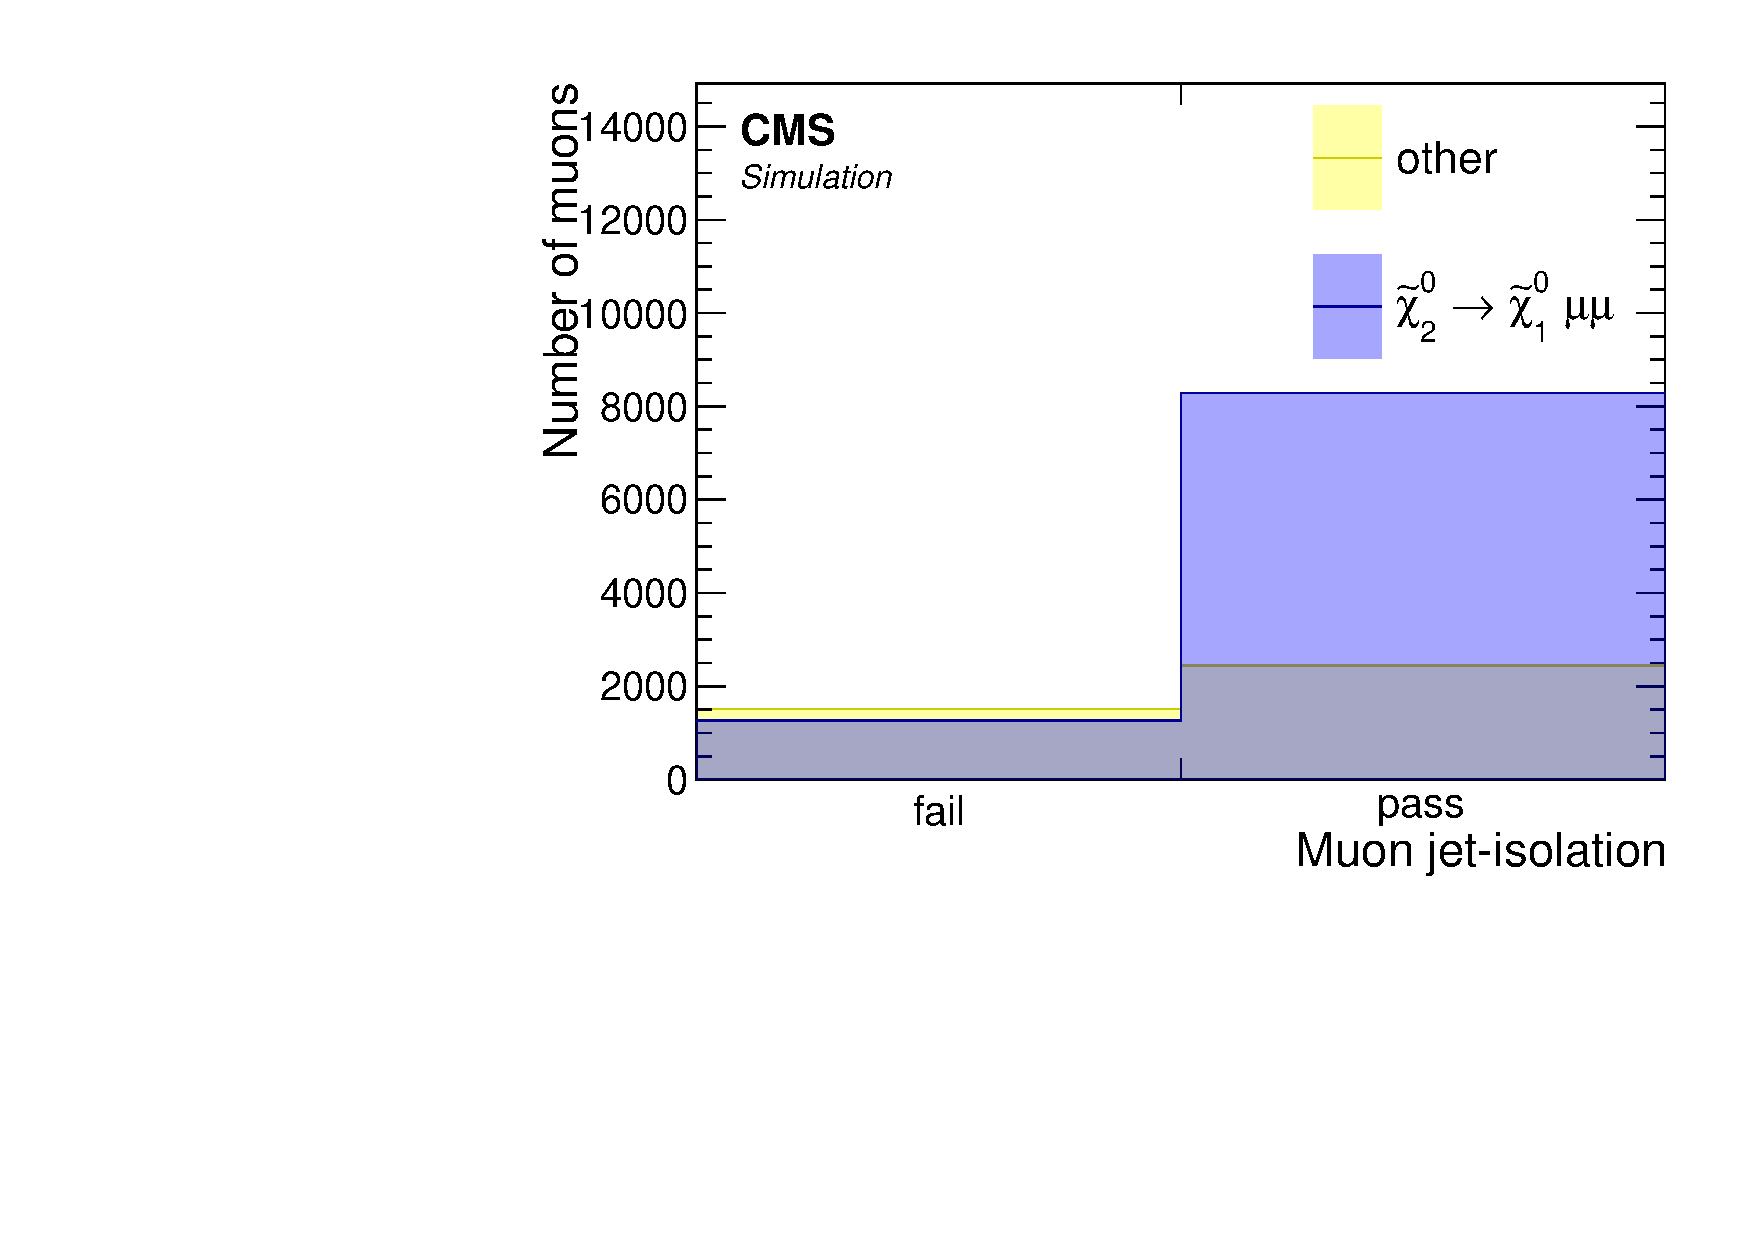
\includegraphics[width=0.32\linewidth]{plots/lepton_selection/lepton_selection_dm1p92/none_Muons_pt_jet_iso.pdf} \,
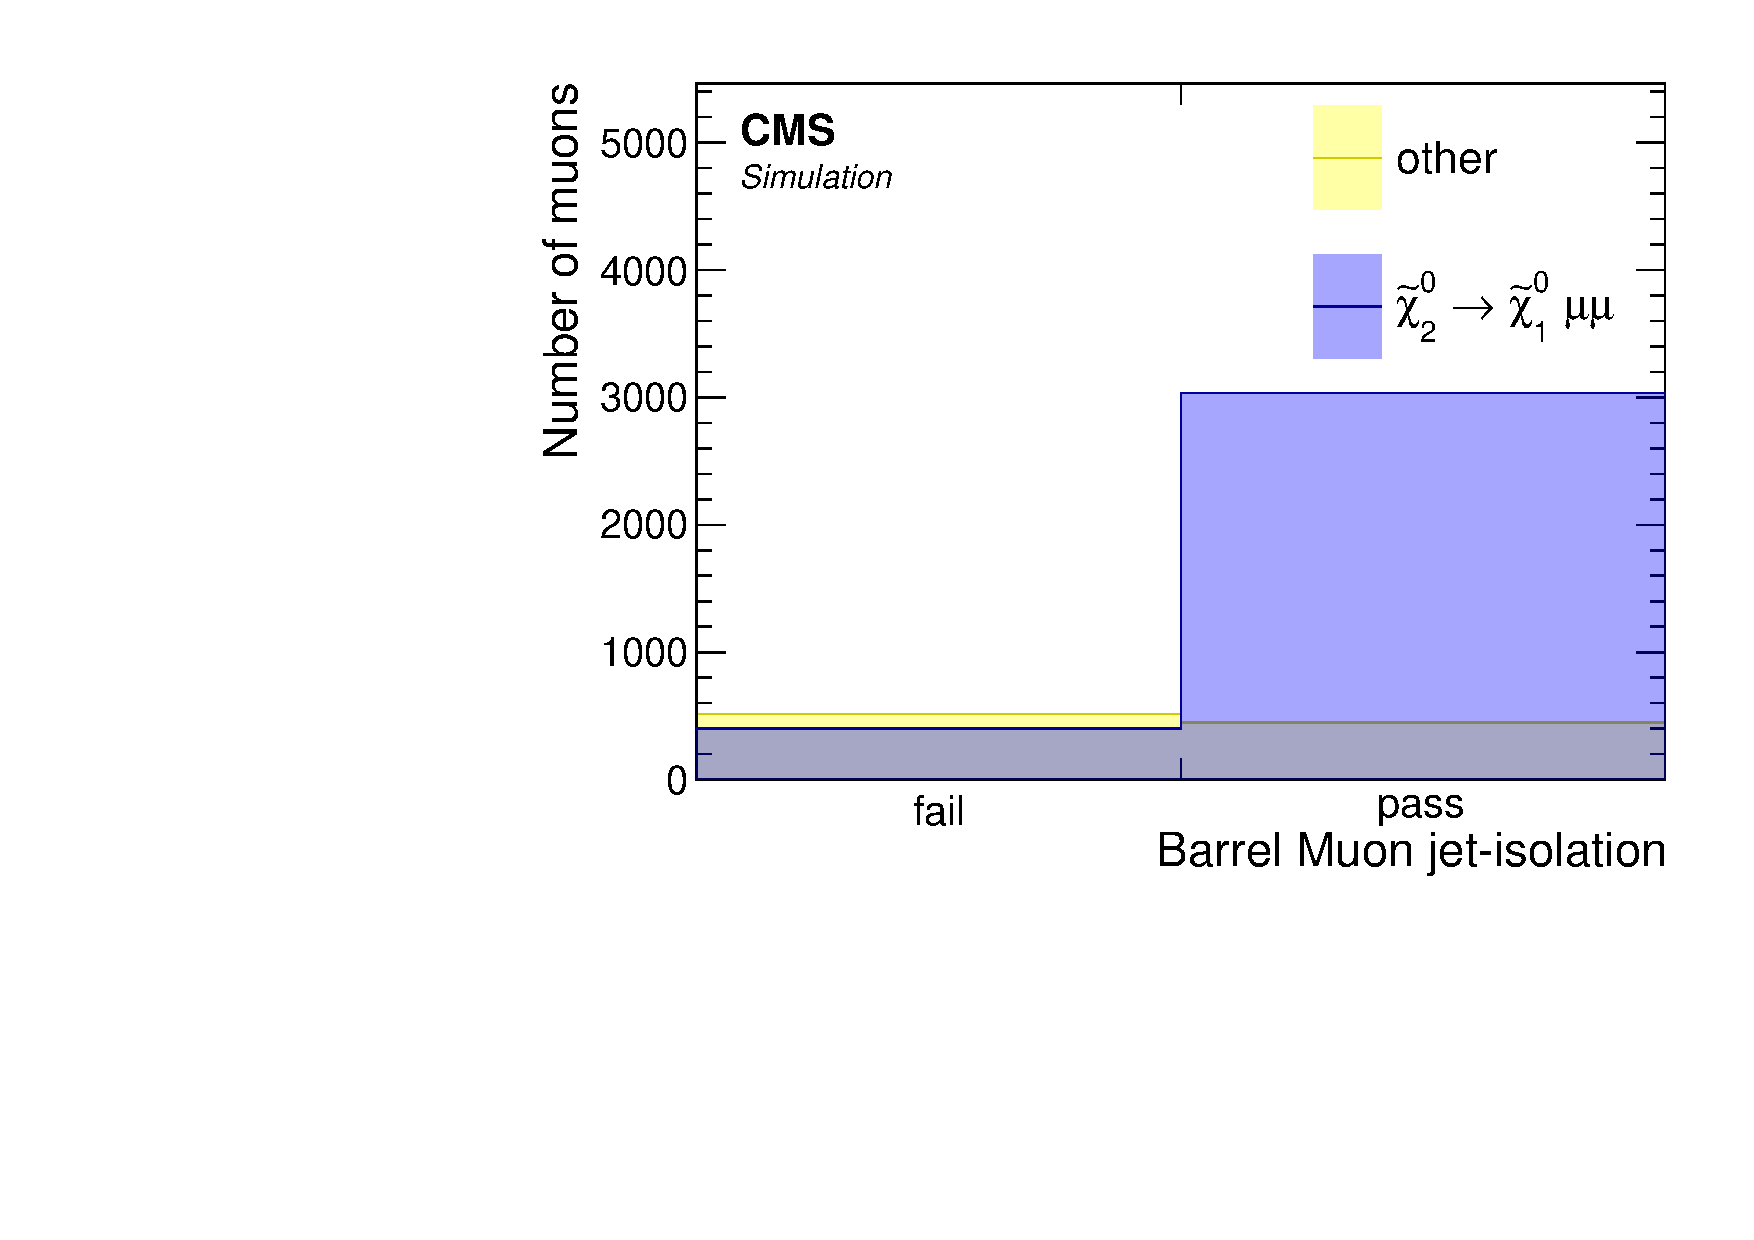
\includegraphics[width=0.32\linewidth]{plots/lepton_selection/lepton_selection_dm1p92/none_Muons_pt_barrel_jet_iso.pdf}  \,
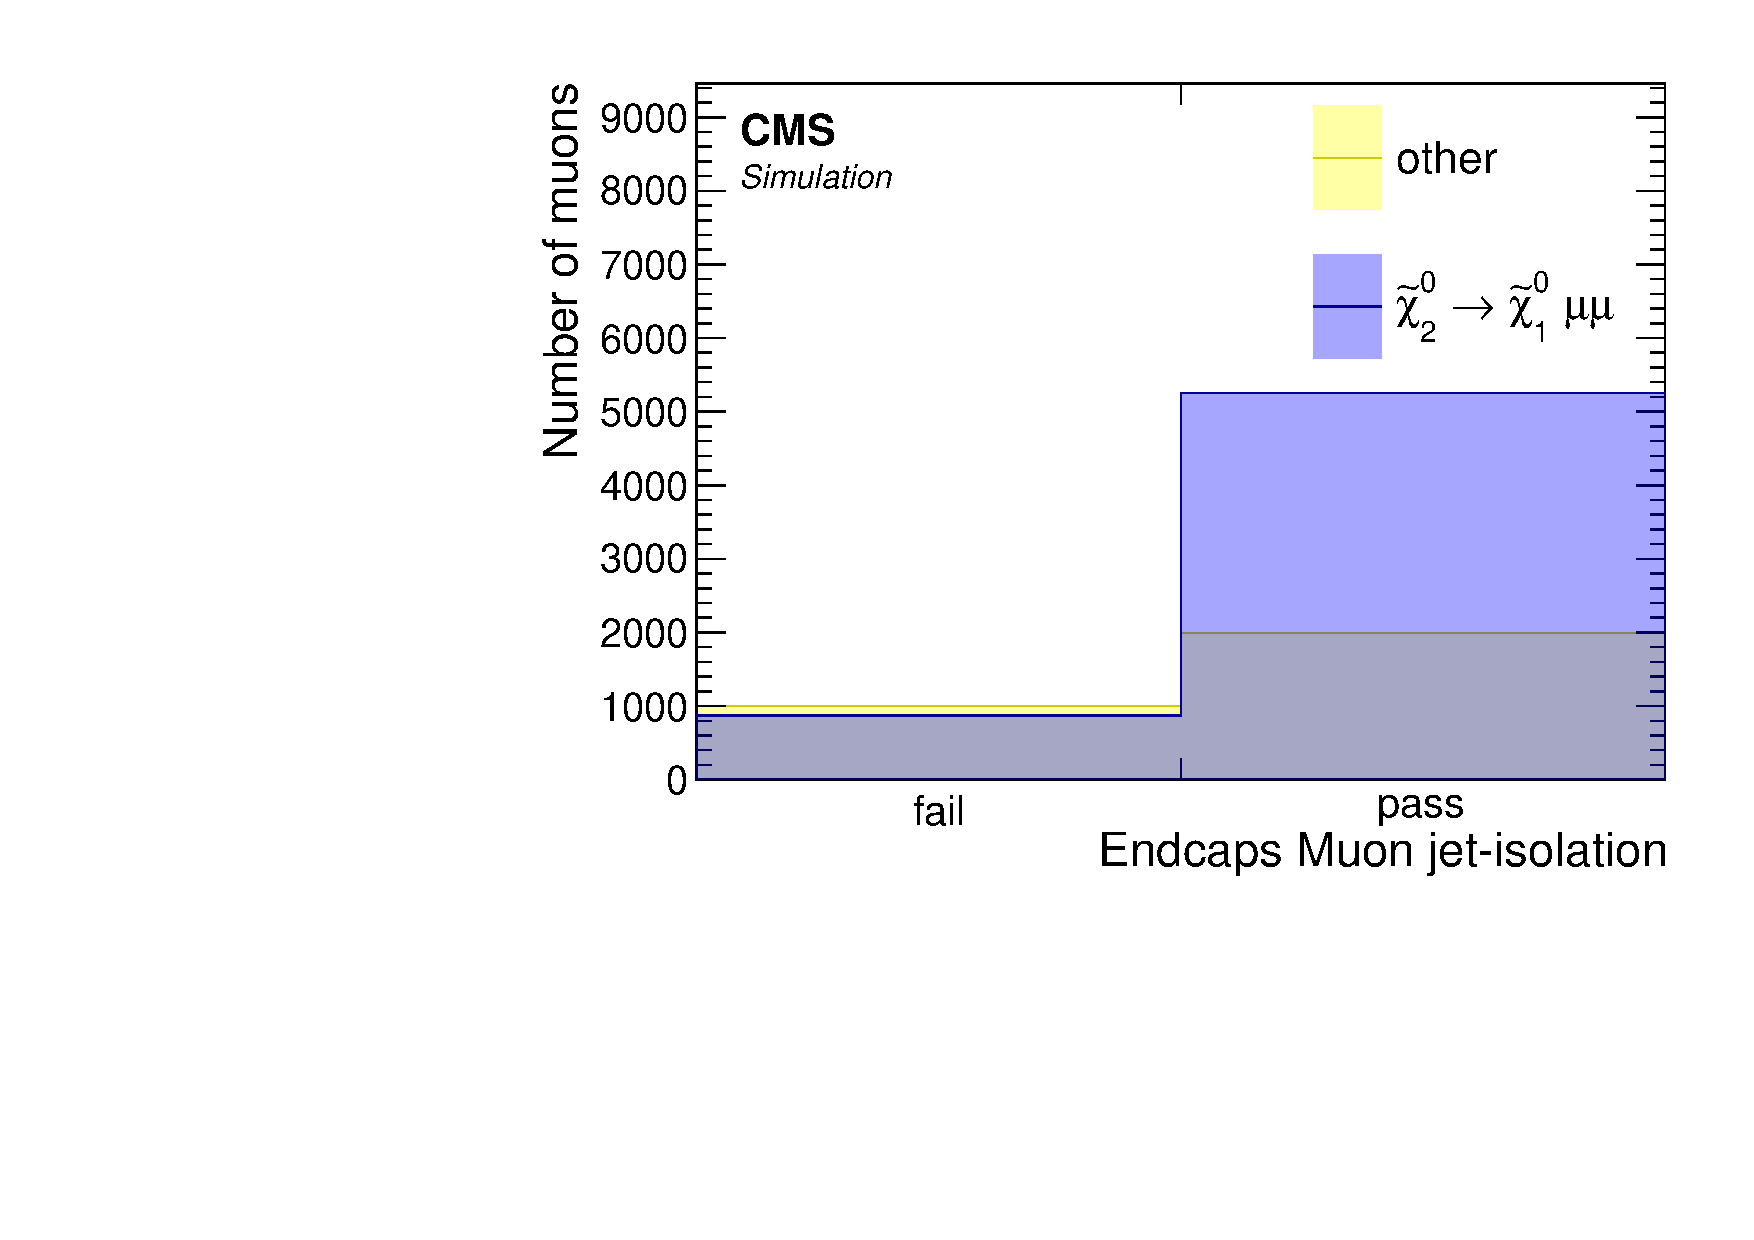
\includegraphics[width=0.32\linewidth]{plots/lepton_selection/lepton_selection_dm1p92/none_Muons_pt_endcape_jet_iso.pdf} \\
\caption[jet-isolation distribution of reconstructed muons]{Jet-isolation distributions of reconstructed muons with medium ID for $\dm=5.63\GeV$ (top) and $\dm=1.92\GeV$ (bottom) in the inclusive \pt case (left), barrel (middle) and endcaps (right). Cuts of $\DR(\jmath_1,\mu)>0.4$, $\pt>2\GeV$ and $\pt<15\GeV$ are applied.}
\label{fig:muons-selection-isolation}
\end{figure}

We summaries this section with the full selection of the analysis muons:
\begin{itemize}[noitemsep]
\item $2<\pt<15\GeV$
\item $\abs{\eta} < 2.4$
\item $\DR(\jmath_1,\mu)>0.4$
\item medium ID working point
\item pass jet-isolation
\end{itemize}


\begin{figure}[]
\centering
\includegraphics[width=0.32\linewidth]{plots/jpsi_muons_fit_bg_delta_r_single_electron/none_invMass_0_0.3_0_1.2.pdf} \,
\includegraphics[width=0.32\linewidth]{plots/jpsi_muons_fit_bg_delta_r_single_electron/none_invMass_0.3_0.5_0_1.2.pdf}  \,
\includegraphics[width=0.32\linewidth]{plots/jpsi_muons_fit_bg_delta_r_single_electron/none_invMass_0.5_1.5_0_1.2.pdf} \\
\includegraphics[width=0.32\linewidth]{plots/jpsi_muons_fit_bg_delta_r_single_electron/none_id_invMass_0_0.3_0_1.2.pdf} \,
\includegraphics[width=0.32\linewidth]{plots/jpsi_muons_fit_bg_delta_r_single_electron/none_id_invMass_0.3_0.5_0_1.2.pdf}  \,
\includegraphics[width=0.32\linewidth]{plots/jpsi_muons_fit_bg_delta_r_single_electron/none_id_invMass_0.5_1.5_0_1.2.pdf} \\
\caption[Barrel BG]{Barrel Muons BG}
\label{fig:tb-barrel-simulation}
\end{figure}

\begin{figure}[]
\centering
\includegraphics[width=0.32\linewidth]{plots/jpsi_muons_fit_bg_delta_r_single_electron/none_invMass_0_0.3_1.2_2.4.pdf} \,
\includegraphics[width=0.32\linewidth]{plots/jpsi_muons_fit_bg_delta_r_single_electron/none_invMass_0.3_0.5_1.2_2.4.pdf} \,
\includegraphics[width=0.32\linewidth]{plots/jpsi_muons_fit_bg_delta_r_single_electron/none_invMass_0.5_1.5_1.2_2.4.pdf} \\
\includegraphics[width=0.32\linewidth]{plots/jpsi_muons_fit_bg_delta_r_single_electron/none_id_invMass_0_0.3_1.2_2.4.pdf} \,
\includegraphics[width=0.32\linewidth]{plots/jpsi_muons_fit_bg_delta_r_single_electron/none_id_invMass_0.3_0.5_1.2_2.4.pdf} \,
\includegraphics[width=0.32\linewidth]{plots/jpsi_muons_fit_bg_delta_r_single_electron/none_id_invMass_0.5_1.5_1.2_2.4.pdf}  \\
\caption[Endcaps BG]{Endcaps Muons BG}
\label{fig:tb-endcaps-simulation}
\end{figure}

\begin{figure}[]
\centering
\includegraphics[width=0.32\linewidth]{plots/jpsi_muons_fit_data_delta_r_single_electron/none_invMass_0_0.3_0_1.2.pdf} \,
\includegraphics[width=0.32\linewidth]{plots/jpsi_muons_fit_data_delta_r_single_electron/none_invMass_0.3_0.5_0_1.2.pdf}  \,
\includegraphics[width=0.32\linewidth]{plots/jpsi_muons_fit_data_delta_r_single_electron/none_invMass_0.5_1.5_0_1.2.pdf} \\
\includegraphics[width=0.32\linewidth]{plots/jpsi_muons_fit_data_delta_r_single_electron/none_id_invMass_0_0.3_0_1.2.pdf} \,
\includegraphics[width=0.32\linewidth]{plots/jpsi_muons_fit_data_delta_r_single_electron/none_id_invMass_0.3_0.5_0_1.2.pdf}  \,
\includegraphics[width=0.32\linewidth]{plots/jpsi_muons_fit_data_delta_r_single_electron/none_id_invMass_0.5_1.5_0_1.2.pdf} \\
\caption[Barrel Data]{Barrel Muons Data}
\label{fig:tb-barrel-data}
\end{figure}

\begin{figure}[]
\centering
\includegraphics[width=0.32\linewidth]{plots/jpsi_muons_fit_data_delta_r_single_electron/none_invMass_0_0.3_1.2_2.4.pdf} \,
\includegraphics[width=0.32\linewidth]{plots/jpsi_muons_fit_data_delta_r_single_electron/none_invMass_0.3_0.5_1.2_2.4.pdf} \,
\includegraphics[width=0.32\linewidth]{plots/jpsi_muons_fit_data_delta_r_single_electron/none_invMass_0.5_1.5_1.2_2.4.pdf} \\
\includegraphics[width=0.32\linewidth]{plots/jpsi_muons_fit_data_delta_r_single_electron/none_id_invMass_0_0.3_1.2_2.4.pdf} \,
\includegraphics[width=0.32\linewidth]{plots/jpsi_muons_fit_data_delta_r_single_electron/none_id_invMass_0.3_0.5_1.2_2.4.pdf} \,
\includegraphics[width=0.32\linewidth]{plots/jpsi_muons_fit_data_delta_r_single_electron/none_id_invMass_0.5_1.5_1.2_2.4.pdf}  \\
\caption[Endcaps Data]{Endcaps Muons Data}
\label{fig:tb-endcaps-data}
\end{figure}

\subsection{Missing transverse energy}
\label{subsec:met}


\clearpage
\subsection{Tracks and multivariate selection }

\begin{figure}[!htb]
\centering
\includegraphics[width=0.48\linewidth]{plots/track_bdt/overtraining_Tracks_Muons_Phase_0.pdf} \,
\includegraphics[width=0.48\linewidth]{plots/track_bdt/overtraining_Tracks_Muons_Phase_1.pdf}  \\
\includegraphics[width=0.48\linewidth]{plots/track_bdt/overtraining_Tracks_Electrons_Phase_0.pdf} \,
\includegraphics[width=0.48\linewidth]{plots/track_bdt/overtraining_Tracks_Electrons_Phase_1.pdf} \\
\caption[Track BDT output plots]{Track BDT output plots for Muons (top) and Electrons (bottom) in phase 0 (left) and phase 1 (right). Blue shows signal tracks, while Red are fake tracks. Test sample overlay on top of training sample.}
\label{fig:track-bdt-output}
\end{figure}

\begin{figure}[!htb]
\centering
\includegraphics[width=0.48\linewidth]{plots/track_bdt/roc_Tracks_Muons_Phase_0.pdf} \,
\includegraphics[width=0.48\linewidth]{plots/track_bdt/roc_Tracks_Muons_Phase_1.pdf}  \\
\includegraphics[width=0.48\linewidth]{plots/track_bdt/roc_Tracks_Electrons_Phase_0.pdf} \,
\includegraphics[width=0.48\linewidth]{plots/track_bdt/roc_Tracks_Electrons_Phase_1.pdf} \\
\caption[Track BDT ROC curves]{Track BDT ROC curves for Muons (top) and Electrons (bottom) in phase 0 (left) and phase 1 (right). Minimum working point showed as a red dot.}
\label{fig:track-bdt-roc}
\end{figure}


\subsection{Isolation}
\label{sec:isolation}
